
% Cal Poly Thesis
% 
% based on UC Thesis format
%
% modified by Mark Barry 2/07.
%




\documentclass[12pt]{ucthesis}
\usepackage{ifpdf} 
%\newif\ifpdf
\ifx\pdfoutput\undefined
    \pdffalse % we are not running PDFLaTeX
\else
\pdfoutput=1 % we are running PDFLaTeX
\pdftrue \fi

\usepackage{textcomp}
\usepackage{url}
\usepackage{algorithmic}
\renewcommand{\algorithmicforall}{\textbf{for each}}
\usepackage{listings}
\lstset{
  language=[Visual]C++,
  keywordstyle=\bfseries\ttfamily\color[rgb]{0,0,1},
  identifierstyle=\ttfamily,
  commentstyle=\color[rgb]{0.133,0.545,0.133},
  stringstyle=\ttfamily\color[rgb]{0.627,0.126,0.941},
  showstringspaces=false,
  basicstyle=\small,
  numberstyle=\footnotesize,
  numbers=left,
  stepnumber=1,
  numbersep=10pt,
  tabsize=2,
  breaklines=true,
  prebreak = \raisebox{0ex}[0ex][0ex]{\ensuremath{\hookleftarrow}},
  breakatwhitespace=false,
  aboveskip={1.5\baselineskip},
  columns=fixed,
  upquote=true,
  extendedchars=true
% frame=single,
% backgroundcolor=\color{lbcolor},
}
\usepackage{color}
%\ifpdf

    \usepackage[pdftex]{graphicx}
    % Update title and author below...
    \usepackage[pdftex,plainpages=false,breaklinks=true,colorlinks=true,urlcolor=blue,citecolor=blue,%
                                       linkcolor=blue,bookmarks=true,bookmarksopen=true,%
                                       bookmarksopenlevel=3,pdfstartview=FitV,
                                       pdfauthor=Christopher Gibson,
                                       pdftitle=Point-Based Color Bleeding With Volumes,
                                       pdfkeywords={thesis, masters, cal poly, volume rendering, global illumination}
                                       ]{hyperref}
    %Options with pdfstartview are FitV, FitB and FitH
    \pdfcompresslevel=1

%\else
%    \usepackage{graphicx}
%\fi

\usepackage{amssymb}
\usepackage{amsmath}
\usepackage[letterpaper]{geometry}
\usepackage[overload]{textcase}



%%%%%\bibliographystyle{abbrv}

\setlength{\parindent}{0.25in} \setlength{\parskip}{6pt}

\geometry{verbose,nohead,tmargin=1.25in,bmargin=1in,lmargin=1.5in,rmargin=1.3in}

\setcounter{tocdepth}{2}


% Different font in captions (single-spaced, bold) ------------
\newcommand{\captionfonts}{\small\bf\ssp}

\makeatletter  % Allow the use of @ in command names
\long\def\@makecaption#1#2{%
  \vskip\abovecaptionskip
  \sbox\@tempboxa{{\captionfonts #1: #2}}%
  \ifdim \wd\@tempboxa >\hsize
    {\captionfonts #1: #2\par}
  \else
    \hbox to\hsize{\hfil\box\@tempboxa\hfil}%
  \fi
  \vskip\belowcaptionskip}
\makeatother   % Cancel the effect of \makeatletter
% ---------------------------------------

\providecommand{\e}[1]{\ensuremath{\times 10^{#1}}}

\begin{document}

% Declarations for Front Matter

% Update fields below!
\title{An Interactive Visualization Model for Analyzing Data Storage System Workloads}
\author{Steven Pungdumri}
\degreemonth{February} \degreeyear{2012} \degree{Master of Science}
\defensemonth{February} \defenseyear{2012}
\numberofmembers{3} \chair{John Oliver, Ph.D.} \othermemberA{Chris Lupo, Ph.D.} \othermemberB{Zo\"{e} Wood, Ph.D.} \field{Electrical Engineering} \campus{San Luis Obispo}
\copyrightyears{seven}



\maketitle

\begin{frontmatter}

% Custom made for Cal Poly (by Mark Barry, modified by Andrew Tsui).
\copyrightpage

% Custom made for Cal Poly (by Andrew Tsui).
\committeemembershippage

\begin{abstract} 

As technology progresses, the rate at which we utilize computer data storage is rapidly increasing, which results in an enormous amount of data being stored and accessed in data centers around the world. The ability to visualize and analyze storage system workloads, specifically bus activity traces between host and storage systems, would be greatly beneficial for storage system developers and administrators seeking to optimize their systems for reliability and efficiency. Inefficiencies in storage system design and administration become apparent with a vast amount of data constantly accessed, such as the algorithms directly pertaining to disk usage both at the software application and embedded hard disk firmware levels. These inefficiencies consequently incur costs associated with failed or underutilized storage media. Captures of storage network activity can provide a window into these systems by gathering meta data that describes the storage accesses occurring over periods of time. However, analyzing and extracting meaningful information from these captures is overwhelming both because of the amount of meta data captured, and the multidimensional, temporal, and spatial characteristics of these datasets.

In this thesis, we develop a system that assists in communicating valuable insights into these datasets, resulting in an approach that utilizes parallel coordinates to model data storage workloads captured with bus analyzers. Users are presented with an effective visualization of workload captures with this implementation, along with methods to interact with and manipulate the model in order to more clearly analyze their storage systems.

Design decisions regarding the feature set of this tool are based on the analysis needs of domain experts and feedback from a conducted user study. Results from our user study evaluations demonstrate the efficacy of our tool to observe valuable insights, which can potentially assist in future storage system design and deployment decisions.

\end{abstract}

\begin{acknowledgements}

First, I would like to thank Dr. Chris Lupo, Dr. John Oliver, and Dr. Zo\"{e} Wood for their help and guidance during my thesis project, as well as for their guidance through my university career. I would also like to thank Dave Hamilton, Scott Olds, David Renuart, and Western Digital who provided a bus analyzer and domain expertise to this ongoing research effort.

Finally, I would like to thank my family for supporting me throughout my university career; I do not know where I would be today without them.

\end{acknowledgements}


\tableofcontents


\listoftables

\listoffigures

\end{frontmatter}

\pagestyle{plain}


\renewcommand{\baselinestretch}{1.66}


% ------------- Main chapters here --------------------

\chapter{Introduction}
\label{intro}

Modeling complex data storage system workloads, specifically bus activity traces between host and storage for analysis, provides an opportunity for storage designers and administrators to interact with and extract information from these complex systems. Analysis from such a model could potentially lead to insights in what is inefficient regarding patterns of disk access, of a particular system design or application~\cite{internal:understanding}. This information would assist in possible areas of failure or underutilization in these complex storage systems, avoiding unnecessary maintenance costs.

\section{Current Methods}
\label{current_methods}

Current bus analyzer software tools often focus on bus protocol rather than providing a broad overview of what is occurring between host and storage. Many of the more sophisticated offerings of bus trace analysis tools are developed in house by corporations interested in optimizing their products or systems, rather than the manufacturers of the bus analyzers. Current methods developed generate graphs which are static and do not allow manipulations to the visualization while viewing the data, lacking functions such as scaling particular areas of interest and highlighting interesting trends. At most, these tools offer various graphs comparing a few dimensions of data at a time, as well as general statistics of the input data~\cite{internal:understanding}. Figure \ref{fig:prev_tool2} illustrates a screenshot of a tool currently utilized by our collaborators in the storage system industry to analyze storage system bus captures, here plotting number of sector and logical block address (LBA) values. While this plot and similar tools have proven effective at analyzing these datasets, they are limited in the amount of data they can display. These tools are simple and prove effective, however it is not possible to view more than a few dimensions of records at once, which is less likely to effectively convey a larger picture of the activity between host and storage.

\begin{figure}[h!]
 \centering
 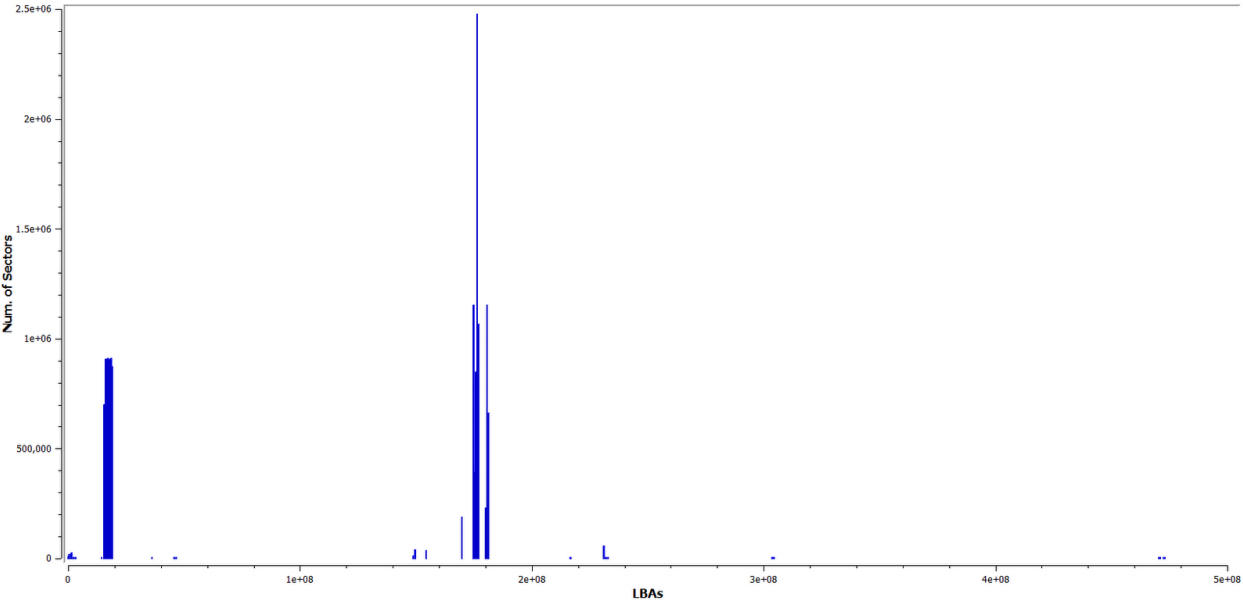
\includegraphics[width=\textwidth]{images/prev_tool2.jpg}
 \caption[Output of a tool currently used to analyze workload datasets.]{Output of a tool currently used by our collaborators to analyze the number of sectors and LBA values from a data storage system bus capture~\cite{internal:collab}.}
 \label{fig:prev_tool2}
\end{figure}

\section{Our Contribution}
\label{contribution}

We propose a tool that incorporates statistical and information visualization techniques, as both an alternative and an addition to current tools available.  An initial statistical analysis of the dataset would yield identified trends and perceived threads, conveyed to the user in the visualization. The user would be presented with an interactive experience in visualizing the bus trace data with our implementation of parallel coordinates---a prominent and effective method of visualizing multi-dimensional datasets. This tool allows the user to manipulate the model through highlighting particular ranges of data,  applying focus+context---an information visualization technique that allows users to more specifically analyze particular areas---on ranges of interest, and applying an overlay to display machine identified threads.  This tool would accommodate bus traces of varying sizes, whether the dataset is a single disk used in a personal computer configuration, or a large-scale data center.

\section{Outline}
\label{outline}
This thesis is organized as follows. In Chapter \ref{initial-work} we begin with smaller, similar dataset from hard disk workloads, intending to extend this approach and knowledge gained to modeling larger data center workloads. We describe our work in pursuing a solution which focuses on the spatial aspects of LBA values in hard disk datasets, however we determine that in order to extensively model large, multi-dimensional datasets of more complex storage systems, parallel coordinates would be more effective. In Chapter \ref{related-works} we present related works in parallel coordinates and how they could contribute towards this domain application. Chapter \ref{data-storage-system-visualization} formally describes our visualization tool and its contributions toward analyzing storage systems, outlining the various functions implemented in the visualization tool. Chapter \ref{results} presents our results after conducting a user study that involves data storage system designers utilizing the tool to analyze a dataset from a corporate data center capture and gathering feedback. In Chapter \ref{future_work} we reflect on our results and describe what future work may entail.

\chapter{Initial Work}
\label{initial-work}

We first research smaller, more manageable datasets of hard disk workloads, in order to develop a visualization approach that could be iterated and extended toward larger data center workloads. Hard disk captures share many of the same dimensions as data center captures, as well as spatial and temporal characteristics. We explore a novel spatial approach to workload captures, with LBA being an important dimension often used to analyze storage system data (as seen in the previous figure), by translating LBA values to physical coordinates to plot the data. This work focused on the visualization of a local hard disk workload capture which could be further extended to captures of a larger, more complex storage system. We thought it would be insightful to observe various attributes of hard disk operations as they spatially occur on the platters. Although there are tools to analyze and view hard disk usage, there are currently none found that provide accurate visualization in the form of physical disk platters present in the drive itself. This previous work set out to map hard disk accesses as accurately as possible, representing each platter contained in an individual drive.

 % This creates opportunities to view other operations of interest, such as cache hits and misses, access times, command types, and more.

\section{Data Storage Analysis Background}
\label{background}

Current commercial implementations of displaying hard disk data consist of pie charts, linear representations of data, and other two and three dimensional graph representations~\cite{internal:requirements}. While these are valuable, observing disk usage spatially provides a novel method of visualizing these datasets, and may present insightful trends that would not be apparent with other methods of modeling captures.

The application we developed uses sample data from a PCMark05 HDD – General Usage test~\cite{pcmark:whitepaper}. Because this testing software is publicly available, this implementation of hard disk modeling would be applicable towards any data output from a capture of the same test. Upon initial analysis of the various dimensions of data captured in this dataset, the LBA dimension and frequency of accesses were identified as more interesting to visualize spatially, and prioritized for this initial visualization.

\section{Approach}
\label{approach}

The primary dimension we aimed to visualize was the frequency of accesses regardless of command type. The LBA would determine the spatial positions of the accesses. The dataset produced by the capture provided multiple dimensions to model in addition to frequency of accesses, however this will be left for future iterations of this work.

\section{Procedure}
\label{procedure}

Our procedure consists of two areas: preparing the data, and determining how to layout and render the data. In our data preprocessing section, we read the dataset into memory and determine the frequency of accesses at each LBA. We then proceed to calculate the spatial position in the visualization, corresponding to variables generated using the dataset when possible, and variables specified by the user when not.

\subsection{Data Preprocessing}
\label{preprocessing}
We began by implementing a parser to read in the data from the input comma separated value (CSV) file containing the workload capture, and designed it to store all of the data available in memory, regardless of its use in this project in order to prepare for future work. The data was then partitioned and stored in a hash table corresponding to the specific head each access occurred on. We decided to specifically utilize a hash table in order to insert and retrieve objects quickly, corresponding to the specific LBA. We utilized the value to be the count of accesses seen throughout the dataset with LBA as the hash table key. We also used a referencing data structure to optimize for only rendering accesses that occurred on the current platter in view.

\subsection{Mapping Data}
\label{mapping-data}

The original design was to implement a Cylinder-Head-Sector (CHS) layout of each platter. Equations converting LBA to the corresponding cylinder, head, and sector are prevalent~\cite{chsmapping:1}\cite{chsmapping:2}. This approach was abandoned however, because although it is a logical method of laying out data on platters, this is not how hard disk access algorithms are implemented today when determining where to write data to disk, due to inefficiency. Figure \ref{fig:chs} illustrates a model of CHS, labeling each part of a head: sector, track, and cylinder. From this figure we can see that each track contains the same number of sectors, regardless of the addition of surface area towards the outside of the head. Because each sector contains the same amount of storage, it is inefficient having a uniform number of sectors across all tracks of the disk, leaving surface area of outer tracks underutilized. 

\begin{figure}[h!]
 \centering
 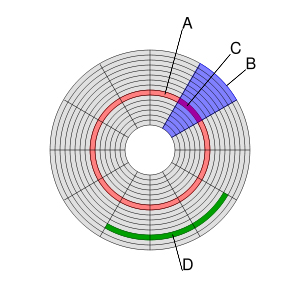
\includegraphics[width=0.5\textwidth]{images/cylinder_head_sector.jpg}
 \caption[A graphical model of a Cylinder-Head-Sector disk layout.]{A graphical model of Cylinder-Head-Sector which illustrates: A) a track, B) a sector, C) a sector of a track, D) a cluster of sectors. This illustrates the inefficiency of CHS by constraining the number of sectors possible in the outer tracks to the number of sectors in the innermost track~\cite{chs:2009}.
}
 \label{fig:chs}
\end{figure}

The Zone-Bit-Recording (ZBR) layout was researched and pursued instead, the idea being that there are various zones across each platter, of which there are a constant or variable number of cylinders with a variable number of sectors depending on the zone. ZBR is illustrated in Figure \ref{fig:zbr} with each zone displayed in a different color. Each track in a particular zone contains the same number of sectors, with more sectors per track as we move outwards on the disk. This layout is used in current hard disks in order to be more spatially efficient in sector density for tracks in zones toward the outside of each disk head~\cite{website:pc_guide}.

\begin{figure}[h!]
 \centering
 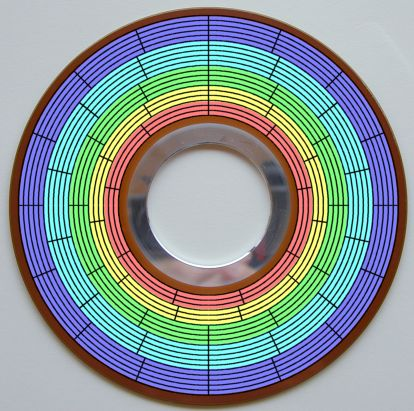
\includegraphics[width=0.5\textwidth]{images/zone_bit_recording.jpg}
 \caption[A graphical model of a Zone-Bit-Recording disk layout.]{A graphical illustration of Zone-Bit-Recording with each zone displayed in a different color. Allowing the outer zone density to be unconstrained from the number of sectors of the inner zones allows for more spatial efficiency, resulting in more capacity~\cite{website:pc_guide}.
}
 \label{fig:zbr}
\end{figure}

The generation of equations to describe the relationships of track to zone, zone to head, and sector to zone are variable between hard disk manufacturers because it can be advantageous to develop more efficient equations relative to competitors. For this initial work, we resorted to calculating equations to represent these relationships by observing trends seen in published data~\cite{quantum:manual}~\cite{ibm:manual}. The decision was to take in a user specified number of zones, tracks per zone, and base sectors per zone to compensate for the variability found across hard disk makes and models. Analyzing the data in tables \ref{table:ibm_data} and \ref{table:quantum_data} proved effective in identifying a trend illustrated in Figure \ref{fig:hard_disk_trends} for the number of sectors per track with respect to the zone, although it did not provide much assistance in a common relationship between the number of tracks per zone in Figure \ref{fig:hard_disk_trends2}, therefore this was left as a constant specified by the user. The decision to use a polynomial equation for the number of sectors per track per zone was a result of the trend observed in the plot in Figure \ref{fig:hard_disk_trends}, with variables provided by the user. This, along with the total number of sectors of the disk (or the highest LBA in the provided dataset) dynamically generates the specific polynomial equation used for mapping data by LBA specific to the input dataset.

\begin{table}[h!]
\begin{center}

\begin{tabular}{|c|c|c|c|}
\hline 
Zone & Tracks in Zone & Sectors Per Track & Data Transfer Rate (Mbits/s)
\tabularnewline
\hline
0 & 624 & 792 & 372.0
\tabularnewline
\hline
1 & 1,424 & 780 & 366.4
\tabularnewline
\hline
2 & 1,680 & 760 & 357.0
\tabularnewline
\hline
3 & 1,616 & 740 & 347.6
\tabularnewline
\hline
4 & 2,752 & 720 & 338.2
\tabularnewline
\hline
5 & 2,880 & 680 & 319.4
\tabularnewline
\hline
6 & 1,904 & 660 & 310.0
\tabularnewline
\hline
7 & 2,384 & 630 & 295.9
\tabularnewline
\hline
8 & 3,328 & 600 & 281.8
\tabularnewline
\hline
9 & 4,432 & 540 & 253.6
\tabularnewline
\hline
10 & 4,528 & 480 & 225.5
\tabularnewline
\hline
11 & 2,192 & 440 & 206.7
\tabularnewline
\hline
12 & 1,600 & 420 & 197.3
\tabularnewline
\hline
13 & 1,168 & 400 & 187.9
\tabularnewline
\hline
14 & 1,815 & 370 & 173.8
\tabularnewline
\hline
\end{tabular}

\captionfonts
\caption[IBM Deskstar 40GV and 75GXP Data]{IBM Deskstar 40GV and 75GXP hard disk data~\cite{ibm:manual}.}
\label{table:ibm_data}
\end{center}
\end{table}

\begin{table}[h!]
\begin{center}

\begin{tabular}{|c|c|c|c|}
\hline 
Zone & Tracks in Zone & Sectors Per Track & Data Transfer Rate (Mbits/s)
\tabularnewline
\hline
0 & 454 & 232 & 92.9
\tabularnewline
\hline
1 & 454 & 229 & 91.7
\tabularnewline
\hline
2 & 454 & 225 & 90.4
\tabularnewline
\hline
3 & 454 & 225 & 89.2
\tabularnewline
\hline
4 & 454 & 214 & 85.8
\tabularnewline
\hline
5 & 454 & 205 & 82.1
\tabularnewline
\hline
6 & 454 & 195 & 77.9
\tabularnewline
\hline
7 & 454 & 185 & 74.4
\tabularnewline
\hline
8 & 454 & 180 & 71.4
\tabularnewline
\hline
9 & 454 & 170 & 68.2
\tabularnewline
\hline
10  & 454 & 162 & 65.2
\tabularnewline
\hline
11 & 454 & 153 & 61.7
\tabularnewline
\hline
12 & 454 & 142 & 57.4
\tabularnewline
\hline
13 & 454 & 135 & 53.7
\tabularnewline
\hline
14 & 454 & 122 & 49.5
\tabularnewline
\hline
\end{tabular}

\captionfonts
\caption[Quantum Fireball Data]{Quantum hard disk data~\cite{quantum:manual}.}
\label{table:quantum_data}
\end{center}
\end{table}

\begin{figure}[h!]
 \centering
 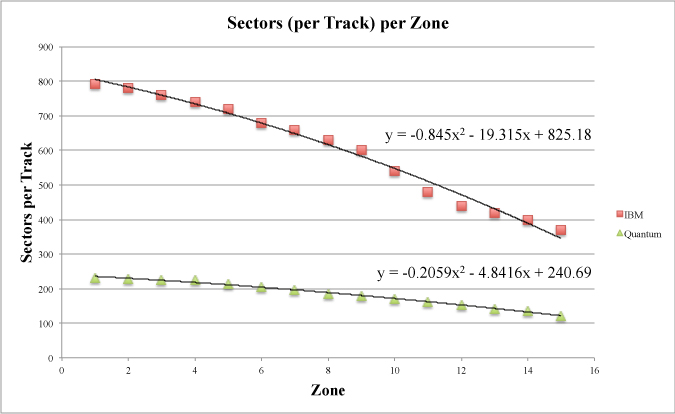
\includegraphics[width=\textwidth]{images/hard_disk_trends.jpg}
 \caption[Observed sectors per track per zone trends from hard disk data.]{Observed sectors per track per zone trends from Quantum and IBM hard disk data.}
 \label{fig:hard_disk_trends}
\end{figure}

\begin{figure}[h!]
 \centering
 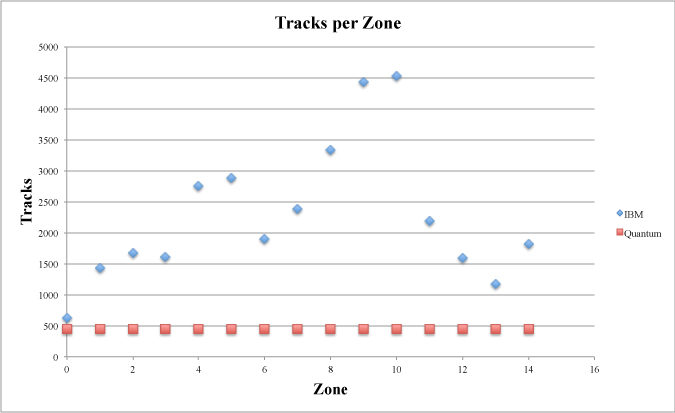
\includegraphics[width=\textwidth]{images/hard_disk_trends2.jpg}
 \caption[Observed tracks per zone trends from hard disk data.]{Observed tracks per zone trends from Quantum and IBM hard disk data.}
 \label{fig:hard_disk_trends2}
\end{figure}

\clearpage

After some work with CHS equations, observed trends and relationships, and other sources of reference, the following equations were derived and implemented to map data points to platters, used each time a specific access was drawn on the model. Again, most of the variables used in these equations were dynamically generated with the values input by the user.

$$Head = \frac{LBA}{Sectors Per Head}$$

$$Zone = \frac{LBA \mod{Sectors Per Head}}{Sectors Per Zone}$$

$$Track = \frac{LBA \mod{Sectors Per Head} \mod{Sectors Per Zone}}{Sectors Per Track}$$

$$Sector = ((LBA \mod{Sectors Per Head}) \mod{Sectors Per Zone}) \mod{Sectors Per Track}$$


\subsection{Graphics}
\label{hard_disk_graphics}

The prevalent computer graphics methods utilized include hierarchical modeling, transformations (virtual trackball implementation), and lighting. Platters were constructed from hierarchical modeling, consisting of a cylinder and two circles rendered above and below. The platter structure was then utilized for drawing the number of disks present (calculated by the number of sectors of the drive and the user input), as well as a primary disk in view, which contained the colored data points. Coloring was determined by mapping each access frequency with a corresponding color, using a simple table of colors ranging from blue to red, corresponding to a simplified rainbow spectrum. Lighting was implemented to convey the physical structure of disk platters, and will be necessary in future iterations of this project if three dimensional data points are drawn to represent other attributes of accesses.

\section{Results}
\label{hard_disk_results}

The result of this project is a working program that takes in a CSV input file, along with following user specified inputs: number of zones, number of tracks per zone, and base sectors per zone. The usage of the tool is as follows:\newline

\noindent diskanalysis [numOfZones] [numOfTracksPerZone] [baseSectorsPerZone] [m] [n]\newline

\noindent With m and n corresponding to the following equation, observed from plotting the data from tables \ref{table:ibm_data} and \ref{table:quantum_data}, shown in Figures \ref{fig:hard_disk_trends} and \ref{fig:hard_disk_trends2}. There is clearly a relationship between sectors per track and zones that can be described with a polynomial equation with varying coefficients, dependent on the hard disk manufacturer and hard disk model. Note that a similar observation was not made between the IBM and Quantum datasets relating tracks per zone, thus a constant is left to the user to specify, following the Quantum data.

$$y = mx^{2} + nx + baseSectorsPerZone$$

Initially, a more accurate geometry was calculated for each sector by rendering polygons with multiple iterations to show curvature of the sector with respect to its position from the center. An early rendering of this without lighting is shown in Figure \ref{fig:initial_disk} where we implemented the CHS layout as well. This approach was abandoned however, in order to optimize the rendering time and to ensure each data point representing an access was of uniform size throughout the dataset, rather than varying with respect to its position from the center of the platter it lies on. As seen in the Figure, the highlighted sector would be smaller than a sector towards the outer edge of the platter, and thus introduce ambiguity when attempting to distinguish between one and many accesses. Although implementing ZBR would make the sectors more uniform than CHS, we decided that individual points to represent each access would be easier to view for large datasets.

\begin{figure}[h!]
 \centering
 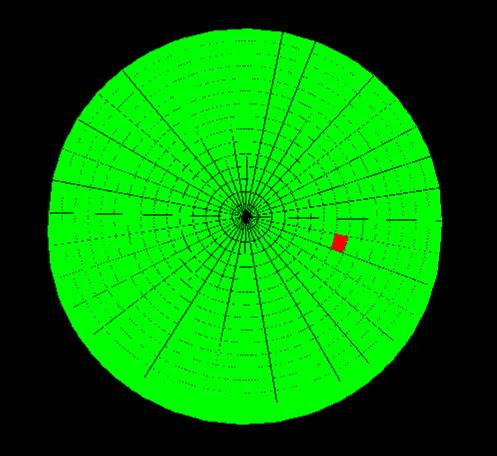
\includegraphics[width=\textwidth]{images/initial_hard_disk.jpg}
 \caption[Screenshot of initial rendering with accurate sector geometry.]{Screenshot of initial rendering with accurate sector geometry and CHS modeling.}
 \label{fig:initial_disk}
\end{figure}

\clearpage

From this, the layout of platters is constructed and drawn with data points representing each access, and a color corresponding to the frequency of accesses. Figure \ref{fig:final_disk} is a screenshot of the application viewing data from a platter of interest. From this visualization, we can observe that the more frequently accessed LBAs in this dataset lie on the outer tracks of the head, illustrated red and orange. LBAs accessed less frequently are colored green, which trail from the red and orange points as we move inner. Then we observe rings of blue, again as we move towards the center of the disk head, conveying that addresses toward the center of the disk tend to be accessed with less frequency. The rings occur because large quantities of data are written to disk sequentially, as the disk read-write head approaches the various sectors of the spinning disk in operation. We also observe that the algorithm that determines LBAs to write to are chosen in a method which results in a spiral-like pattern, again for large sequential writes. These findings sensibly correspond with our knowledge of hard disks, for instance the fact that the read-write head begins its path from the outer tracks of the platter, inwards. An algorithm which stores more frequently accessed data in the outer tracks would thus result in less overall movement of the support arm for the read-write head during the lifetime of the hard disk, potentially yielding greater disk reliability.

\begin{figure}[h!]
 \centering
 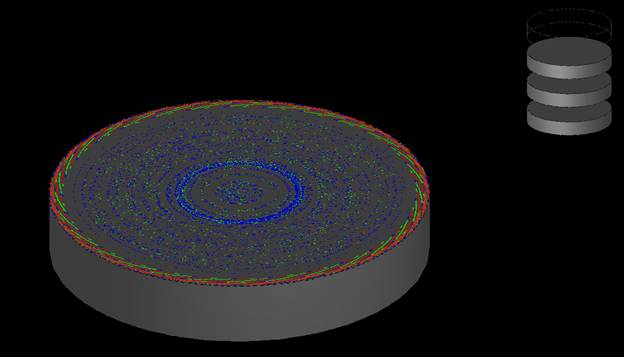
\includegraphics[width=\textwidth]{images/final_hard_disk.jpg}
 \caption{Screenshot of the final application observing a platter.}
 \label{fig:final_disk}
\end{figure}

Future work in modeling data spatially will consist of more research to obtain more accurate equations and values to map data points. Work can also include furthering the analyzing and displaying of other dimensions of interest, possibly with the use of utilizing a third dimension on each disk head. 

Visualizing data storage system captures is difficult because the datasets are multidimensional, temporal, and spatial, allowing many approaches of promising visualization methods. From this initial work, we became more accustomed to the dataset, specifically LBA values and an insight into hard disk access algorithms for writing to disk. Although this was a novel approach at visualizing data storage captures, it contains a few important shortcomings to note: it is based on equations generated from observing hard disk characteristics and user input, which is not completely accurate without the cooperation of hard disk manufacturers to obtain specific equations to more accurately model them. More importantly, this approach is limited in its ability to clearly visualize additional dimensions and larger datasets, particularly captures of data center activity, rather than individual hard disks. To model such captures, parallel coordinates is a promising approach because it accommodates multidimensional, large datasets by design, as opposed to our approach with modeling individual hard disks and platters in a visualization which effectively displays much fewer dimensions. From this previous work, we were able to build our knowledge on storage system captures and develop techniques in parsing and architecting data structures for these storage datasets, knowledge upon which we developed our following tool in parallel coordinates.

\chapter{Related Works in Parallel Coordinates}
\label{related-works}

We begin our work with parallel coordinates by first researching related works and implementations in order to see what may be applicable to our datasets. Each of these efforts center around novel techniques in addition to parallel coordinates when visualizing datasets of specific domains in particular, some of which may apply to data storage system workload captures as well.

\section{Parallel Coordinates Background}
\label{background}

Parallel coordinates is a method of visualizing multi-dimensional datasets. Each dimension of data is represented by a parallel axis in the model. Records in the dataset are illustrated as a point on each dimension, with the position on the axis corresponding to its value in the particular dimension. Further, the collection of points for each record are connected with line segments between each pair of adjacent axes, resulting in a polyline across the set of dimensions for each record in the dataset. This basic implementation of parallel coordinates has been prevalently used as an effective technique for modeling multi-dimensional datasets in various areas of research~\cite{Inselberg:1990:PCT:949531.949588}.

Areas of further research commonly entail the implementation of an additional approach for user interaction or mode of visualization which makes the overall tool more effective pertaining to datasets in a particular area of research. Each specific domain application has its own requirements with each contribution of research, and that certain methods that are extremely effective on datasets of one area, may not be effective at all on datasets of another~\cite{novotny:2006:OPFC}~\cite{johansson:2007:DCDTPC}~\cite{peng:2005:CRMD}~\cite{Graham:2003:UCE}. This section describes a few related works with novel additions to parallel coordinates, designed for datasets of other areas of interest, some more likely useful for modeling data storage system captures as opposed to others.

\section{Data Binning}
\label{data_binning}
Data binning is a preprocessing technique that quantizes data by categorizing the original data points as bins as they fall within specified intervals~\cite{website:binning}. Using this technique for large datasets can effectively convey trends, at the cost of less resolution.

Novotny and Hauser were effective in illustrating context and outliers by applying a binned data method~\cite{novotny:2006:OPFC}. This implementation used a preprocess data binning approach to identify common trends between each pair of dimensions, which made it easier to visually comprehend these trends as well as reducing the load on rendering by using parallelograms for each grouping, rather than individual polylines. They proceeded to identify outliers by leveraging their data binning and rendered these with the typical approach of using polylines to ensure their distinction, and rendered the user specified focus (brushing) with the same method as well. Figure \ref{fig:data_binning} illustrates a flow simulation dataset of two fluids mixing, rendering prominent parallelograms representing bins of data, as opposed to the higher resolution of individual polylines.

This implementation of parallel coordinates would be effective for any general dataset that requires the identification of trends, outliers, and user focus. As with any approach that decreases data resolution, information can be obfuscated as well. Data binning would be a promising area to investigate for the future work of our tool.

\begin{figure}[h!]
 \centering
 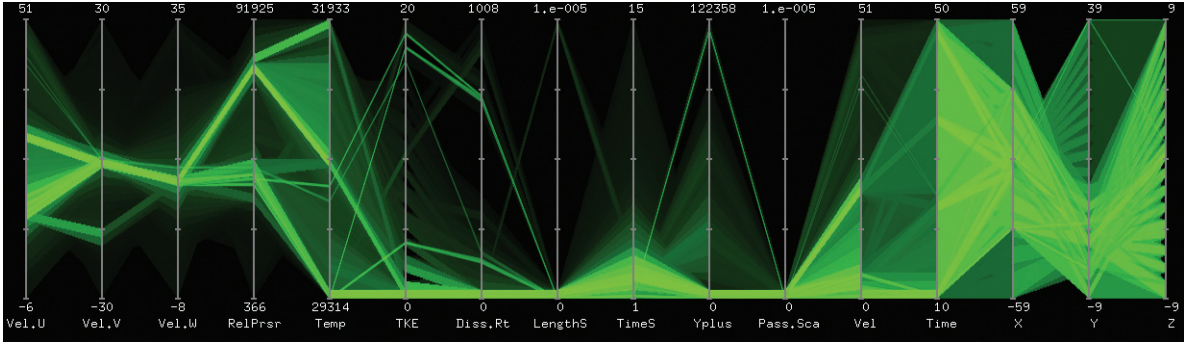
\includegraphics[width=\textwidth]{images/data_binning.jpg}
 \caption[Data bins rendered as polygons rather than individual polylines.]{Data bins rendered as polygons rather than the standard plot with individual polylines.}
 \label{fig:data_binning}
\end{figure}

\section{Temporal Depth Cues}
\label{temporal_depth_cues}

Storage system workloads are both spatial and temporal. While we initially explored the spatial aspects of our dataset, analyzing the changes across time may produce insights that would be less apparent otherwise.

Johansson et al. investigate the illustration of depth cues in temporal parallel coordinates~\cite{johansson:2007:DCDTPC}. This research produced a temporal window by constructing density maps and utilizing transfer functions. A depth cue visualization was produced based on temporal binning, perception based coloring, and concepts from volume rendering. In Figure \ref{fig:temporal_depth} we see an example of visualizing a large, time-varying, multivariate dataset, rendering polygons when the size of changes between time steps increases.

This approach does not seem as effective when applied to a data storage analysis capture where informative discoveries lie in the identification of common trends and outliers found in the dataset at all points in time, because the value from an in-depth temporal analysis would illustrate how significant the dataset changes over varying time periods.

\begin{figure}[h!]
 \centering
 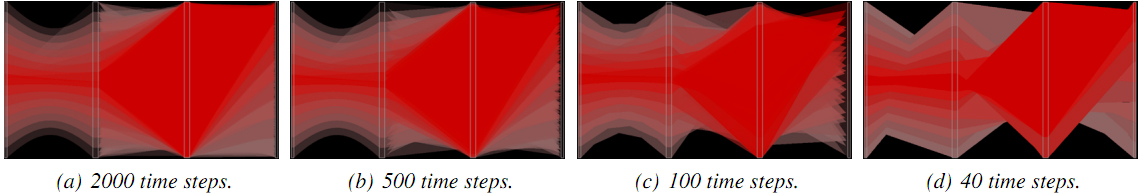
\includegraphics[width=\textwidth]{images/temporal_depth.jpg}
 \caption{Temporal depth cues used to convey time-varying multivariate data.}
 \label{fig:temporal_depth}
\end{figure}

\section{Dimension Reordering}
\label{dimensional_reordering}
Ordering of dimensions can be important with visualizing multidimensional datasets. It is difficult to manually determine what the most effective arrangement is with many dimensions; this can depend on characteristics of the data being analyzed, as well as the information the user intends to extract from it.

Dimension reordering is another area of parallel coordinates researched to reduce clutter in visualizations~\cite{peng:2005:CRMD}. Although most implementations of parallel coordinates allow manual reordering, this can be exhaustive when searching for a more effective ordering of dimensions. This particular implementation defined a metric used to measure the amount of clutter, and applied it to all possible arrangements to identify the one with the least amount of clutter. This metric relies on normalized Euclidean distances between data points and a user adjustable threshold to determine the sensitivity of clutter detection. From here, a few algorithms were proposed for optimally searching for the least cluttered arrangement. 

While this is an interesting approach, we would like to accumulate more feedback from experts in our data storage system domain to analyze if any trends appear for the arrangement of dimensions that is most effective, and whether it correlates to the amount of clutter observed before incorporating this functionality in our tool. Ultimately, manually analyzing variations in ordering for the nineteen dimensions in our datasets is not feasible, therefore an automated approach such as this would be a beneficial area of future work.

\section{Visualization Enhancing Curves}
\label{curves}
An ambiguity often found in basic implementations of parallel coordinates is when a common point is shared among multiple records, making it difficult to establish which direction each of the records proceeds on towards the adjacent dimension. When following a record preceding the intersecting point on a dimension, the resulting polyline could be any of the polylines stemming from the intersection at the dimension.

This particular implementation resolves this conflict with curves instead of polylines, which hints to human visual processing at the resulting direction of each record by following the best fit curve matching to its preceding counterpart~\cite{Graham:2003:UCE}. Figure \ref{fig:curves1} illustrates a dataset of individuals and their career qualifications gathered from a research project that intends to assist businesses in forming project groups for particular projects. This Figure demonstrates the use of curves, as opposed to polylines for clarification at points of intersection on each dimension. 

\begin{figure}[h!]
 \centering
 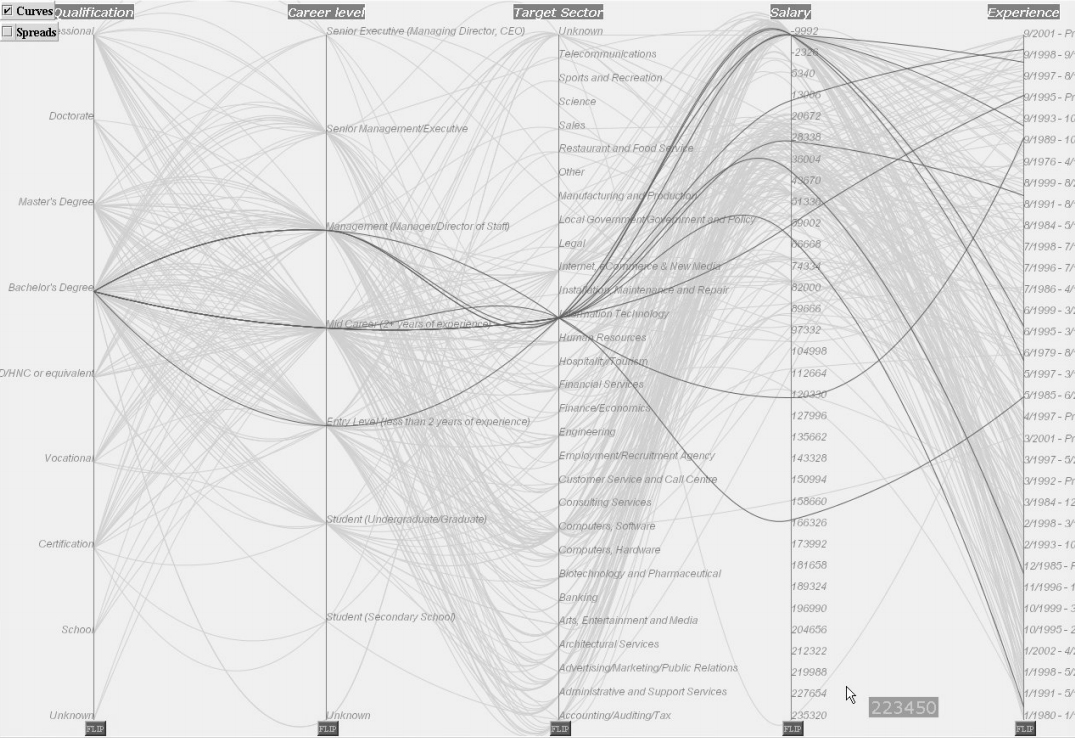
\includegraphics[width=\textwidth]{images/curves.jpg}
 \caption[Curves used to address crossover uncertainties.]{Curves used to address crossover uncertainties when records share a crossover point on a dimension.}
 \label{fig:curves1}
\end{figure}

A focus+context feature further spreads these records and includes a bounding box to indicate if a point with multiple records has been spread. The repositioning is calculated by moving the dimensional crossing point proportionally to its average position in the preceding and following dimensions, a technique which can be accomplished without curves as well. The spreading technique is illustrated in Figure \ref{fig:curves2}, first showing an example without spread at an intersection, then spreading at the same intersection with a bounding box to convey the original point of intersection. The rendering of curves as opposed to polylines comes at the expense of performance, requiring optimizations in data preprocessing as well as repainting algorithms.


\begin{figure}[h!]
 \centering
 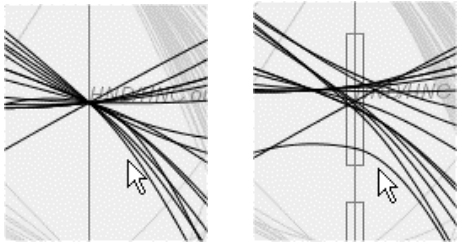
\includegraphics[width=0.5\textwidth]{images/spread.jpg}
 \caption[Spreading at a crossover point to display individual data records.]{An initial implementation without spreading at a crossover dimension point, followed by spreading at the same point to clearly display individual data records.}
 \label{fig:curves2}
\end{figure}

This approach seems promising, however it will be left as future work after extensive user feedback to assess the current level of clarity at crossover points across dimensions. From there, it can be determined if the benefits found in this work could extend to modeling data storage system workloads.

\section{Common Objective}
\label{common_objective}
Each of these prior additions to parallel coordinates are novel and intended to more effectively model the datasets from particular areas of specific domain applications they chose to visualize, or modeling large datasets in general. From this research, we are presented with effective methods to enhance parallel coordinates and more clearly visualize large, multidimensional datasets.

When focusing on a specific area with which to obtain a dataset as opposed to attempting to develop a general purpose visualization tool, it is beneficial to consult domain experts in order to gather requirements to address relevant pain points in order to effectively contribute towards that particular area of research. We gathered specific requirements from Western Digital with respect to modeling captures from data storage systems by observing what their current tools aid them in, and inquiring what they as domain experts would find interesting to be able to observe. We implemented our addition to parallel coordinates from our observations, that addresses their current needs as well as functionality anticipated to be valuable when analyzing their datasets.

\chapter{Data Storage System Visualization}
\label{data-storage-system-visualization}

We present an information visualization tool that analyzes data storage system workloads through bus analyzer captures. This tool is intended for storage system designers, administrators, and others interested in gaining insight in these workloads. Our tool allows users to model bus analyzer captures of data storage system workloads, and provides the following feature set.

\section{Dataset Overview}
Our input dataset output is in CSV format, output from bus analyzer preprocessing software. The values to be expected are both integers and floating point numbers for continuous dimensions, and particular character strings for discrete axes, which are hardcoded as constants expected when preprocessing the input data. Users begin the visualization with an overview of all storage commands displayed using traditional parallel coordinates. All axes are defaulted to being shown; they can be hidden or revealed at any point, as well as rearranged for more relevant comparisons between axes. Axes can be displayed with either a linear or logarithmic scale, and particular dimensions are defaulted as such in order to display the spread of values more effectively according to the nature of the dimension. At any point, the user can perform transformations on the model including scaling in and out, as well as translations vertically or horizontally. Figure \ref{fig:overview} displays a sample storage system workload capture with the initial overview mode, displaying all records and dimensions of the dataset. Each of the nineteen dimensions of these datasets illustrated in our visualization are listed and described below~\cite{internal:requirements}.

\begin{itemize}
\item \textbf{Time} - a floating point number that represents the time in seconds that the command was received by the storage device.

\item \textbf{End Time} - a floating point number that represents the time in seconds that the command was completed by the storage device.

\item \textbf{Command ID} - an integer that represents the order of which the command was received by the storage device.

\item \textbf{End Command ID} - an integer that represents the order of which the command was completed by the storage device.

\item \textbf{Intercommand Time} - a floating point number that represents the time in milliseconds that the host system takes to issue a new command to the storage device.

\item \textbf{Logical Block Address} - an integer containing the starting logical block address of the command.

\item \textbf{Command Length} - an integer containing the length of the command.

\item \textbf{Command Completion Time} - a floating point number that represents the time in milliseconds from when the command is received by the storage device, and the time the command is completed.

\item \textbf{Queue Command Completion Time} - a floating point number that represents the completion time in milliseconds of command relative to others in the queue.

\item \textbf{Queue Depth} - an integer that contains the queue depth when the command is received.

\item \textbf{End Queue Depth} - an integer that contains the queue depth when the command is complete.

\item \textbf{FIFO Position} - an integer that contains the position in the queue from the host perspective when the command is executed.

\item \textbf{Stream Number} - an integer that contains the stream which the command belongs.

\item \textbf{Queueable} - a boolean value that signals if the command was sent to the storage device as a command that can be queued. 

\item \textbf{Command Type} - a character string that identifies the type of command sent to the storage device.

\item \textbf{Alignment} - a character string that describes the alignment properties of the command.

\item \textbf{Forced Unit Access} - a boolean value that signals if the command is a forced unit command.

\item \textbf{Sequential} - a character string that describes whether the command is sequential to the previous command that was received, part of a sequential stream, or not sequential to the previous command that was received.

\item \textbf{Cache Hit} - a character string that describes whether the command is a possible cache hit, determined by the command completion time.
\end{itemize}

\begin{figure}[h!]
 \centering
 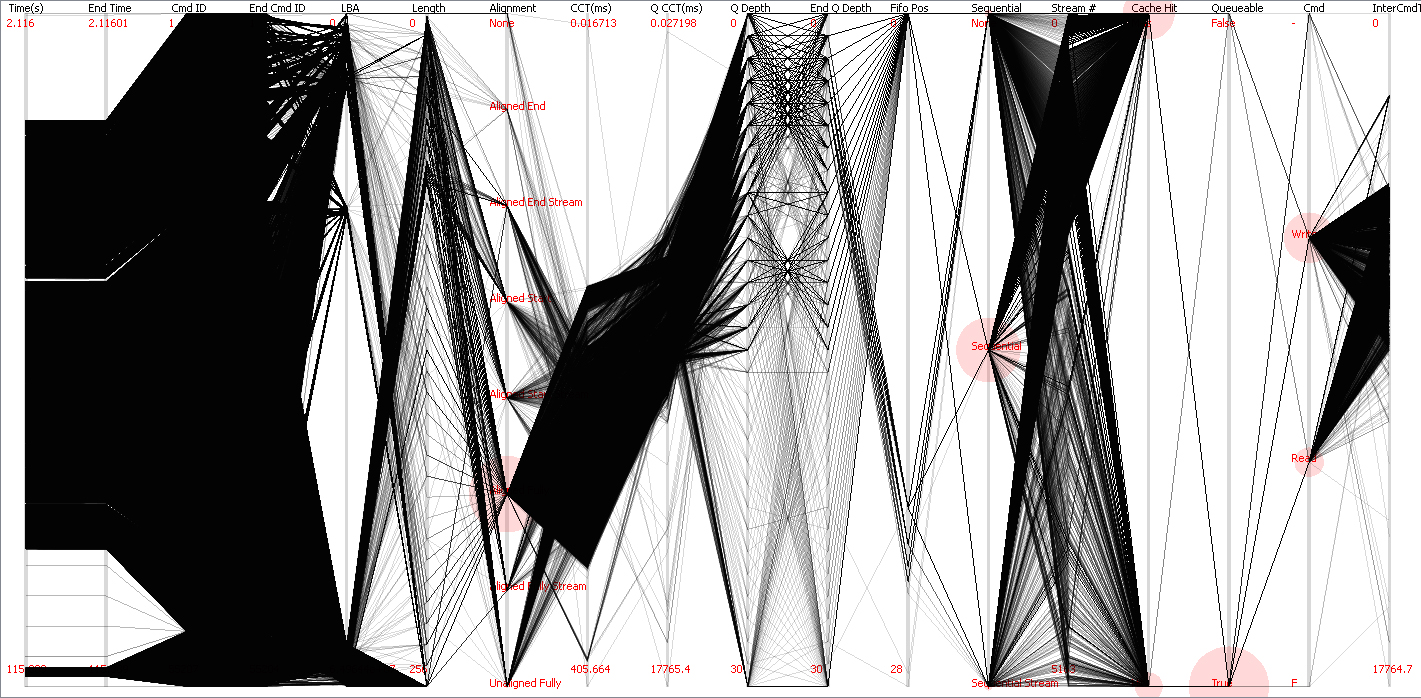
\includegraphics[width=\textwidth]{images/overview.jpg}
 \caption[Overview mode of a sample storage system workload dataset.]{Overview mode of a sample storage system workload dataset with all dimensions displayed.}
 \label{fig:overview}
\end{figure}

\section{Continuous Axes}
Most axes are categorized as containing continuous values, containing numerical values that span across the dimension. When a user focus is applied, the minimum and maximum values for continuous axes are adjusted to those of the focus in order to spread the values specifically in the area of interest. Each of the continuous axes in storage system datasets are listed below.

\begin{tabular}{p{0.5\textwidth}p{0.5\textwidth}}
\begin{itemize}
\item Time
\item End Time
\item Command ID
\item End Command ID
\item Intercommand ID
\item Logical Block Address
\item Stream Number
\end{itemize}
&
\begin{itemize}
\item Command Length
\item Command Completion Time
\item Queue Command Completion Time
\item Queue Depth
\item End Queue Depth
\item FIFO Position
\end{itemize}
\end{tabular}

\section{Discrete Axes}
Particular axes, namely: Queued, Command, Alignment, Forced Unit Access (FUA), Sequential, and Cache Hit are recognized as axes with discrete values. This is taken into account when parsing input data and displaying the visualization, primarily by hardcoding the character string values and assigning a numerical value when storing the dataset. Discrete axes will display the full range of the possible values found in the dataset regardless of the current user set focus (although the values themselves will not be visible if they are outside of the user set focus). The possible values and descriptions for these axes are listed below.

\noindent \textbf{Alignment}
\begin{itemize}
\item None - this command alignment is undetermined.
\item Aligned End - this command starts unaligned, but ends aligned.
\item Aligned End Stream - this command is part of a sequential stream that starts unaligned, but ends aligned.
\item Aligned Start - this command starts aligned, but ends unaligned.
\item Aligned Start Stream - this command is part of a sequential stream and starts aligned, but ends unaligned.
\item Aligned Fully - this command starts and ends aligned.
\item Aligned Fully Stream - this command is part of a sequential stream that starts and ends aligned.
\item Unaligned Fully - this command starts and ends unaligned.
\end{itemize}

\noindent \textbf{Cache Hit}
\begin{itemize}
\item Miss - this command is a cache miss.
\item Hit - this command is a possible cache hit.
\end{itemize}

\noindent \textbf{Command Type}
\begin{itemize}
\item (-) - this is a miscellaneous power management command to the storage device.
\item Flush Cache - this is a command that signals the storage device to flush its cache.
\item Read - this is a command to read data from the storage device.
\item Write - this is a command to write data to the storage device.
\end{itemize}

\noindent \textbf{Forced Unit Access}
\begin{itemize}
\item False - this command is not a forced unit access, data may be accessed from a cached copy.
\item True - this command is a forced unit access, data must be accessed from the storage media surface and not attempt to use the cache.
\end{itemize}

\noindent \textbf{Queueable}
\begin{itemize}
\item False - this is a command that cannot be queued.
\item True - this is a command that can be queued.
\end{itemize}

\noindent \textbf{Sequential}
\begin{itemize}
\item None - this is a command that is not sequential to the previous command that was received.
\item Sequential - this is a command that is sequential to the previous command that was received.
\item Sequential Stream - this is a command that part of a stream of sequential commands.
\end{itemize}

\section{Circular Histograms}

Another defining feature of our visualization is circular histograms, which illustrate point distribution frequencies along discrete axes. Previous attempts at more effectively illustrating the density of one to many values on particular dimensions as well as clarifying crossover ambiguity include the use of curves and point spread \cite{Graham:2003:UCE}, context generation \cite{novotny:2006:OPFC}, and basic overlays of histograms. Figure \ref{fig:histograms} illustrates an example of overlayed histogram bars, which can be distracting and complicate the overall view of individual records. We decided to avoid point spreading as shown in Figure \ref{fig:curves2} because it can potentially mislead the user with deliberately altered point positions, and favor an underlying histogram approach in order to preserve the significance of the command values rather than the histograms themselves. Initially we implemented traditional histogram rectangles, but found they were hard to observe for particular values with more dense spreads. We instead implement circular histograms with radii corresponding to the proportional ratio for each sum of discrete values in the dataset (constrained to the user specified focus if applied). This approach preserves both the significance of the command values, as well as the illustration of trends across discrete axes, illustrated in Figure \ref{fig:histograms}. From this Figure, it becomes clear that there were more cache hits occurring, a high percentile of accesses were queueable, and that more writes occurred as opposed to reads in this particular dataset. These observations would not be easily perceived without the visual aid of histograms.

\begin{figure}[h!]
 \centering
 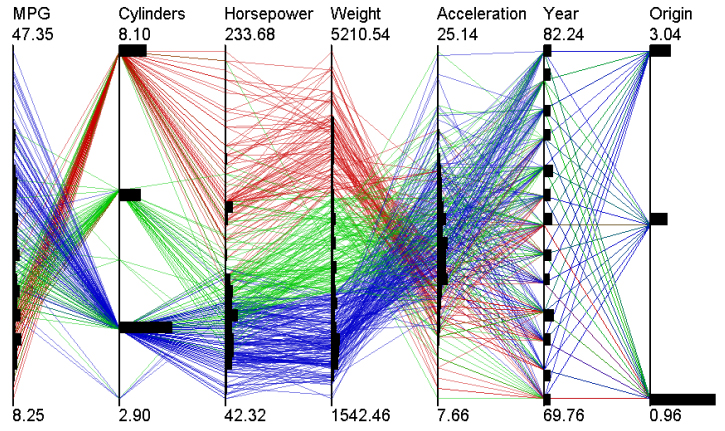
\includegraphics[width=\textwidth]{images/histograms.jpg}
 \caption[Parallel coordinates visualization with histogram bars overlayed.]{Parallel coordinates visualization of a car dataset with histogram bars overlayed at point distributions along axes~\cite{McDonnell_Mueller_2008}.}
 \label{fig:histograms_ex}
\end{figure}

\begin{figure}[h!]
 \centering
 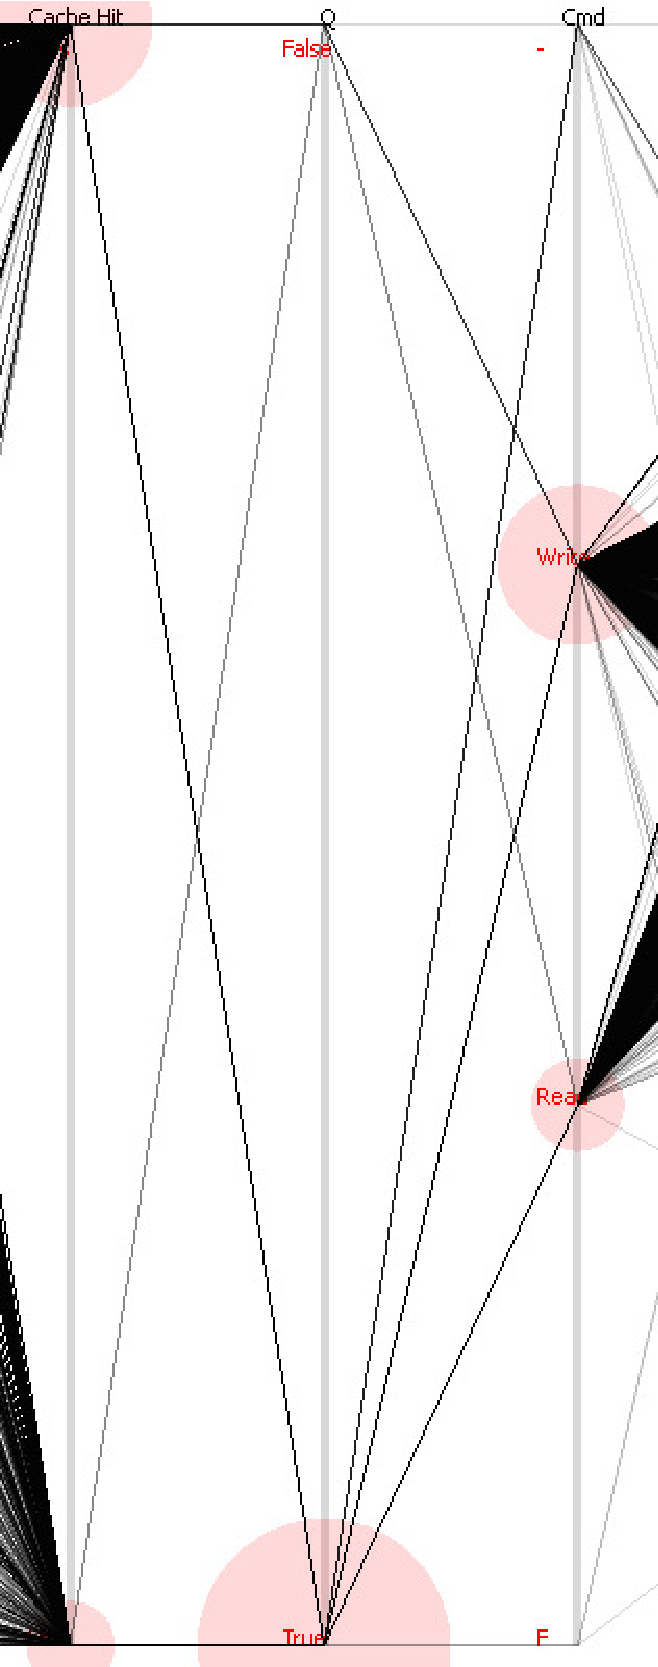
\includegraphics[width=0.5\textwidth]{images/discrete.pdf}
 \caption{Discrete axes illustrated with circular histograms to convey trends.}
 \label{fig:histograms}
\end{figure}

\section{Focus+Context}
Users have two methods of applying focus to the visualization, brushing a range of data on a particular axis and applying a user specified focus on a particular axis, both which extend to the rest of the axes.

\subsubsection{Brushing}
Brushing is a common feature in parallel coordinates that allows users to brush a particular range on an axis a distinct color. Users can apply this technique that will extend to other axes and brush all commands that fall under the scope selected. Figure \ref{fig:brush} illustrates the use of brushing, and from this we can analyze the accesses which occur in the second half of our capture, and notice that within this subset of data highlighted, queue depth values remain in the lower range in comparison to the rest of the data rendered in black. In Figure \ref{fig:brush2}, we apply brushing to all write commands and observe that the beginning portion of our capture consisted mostly of write commands. Furthermore, we notice that a majority of the write commands in this dataset are definitive cache misses.

\begin{figure}[h!]
 \centering
 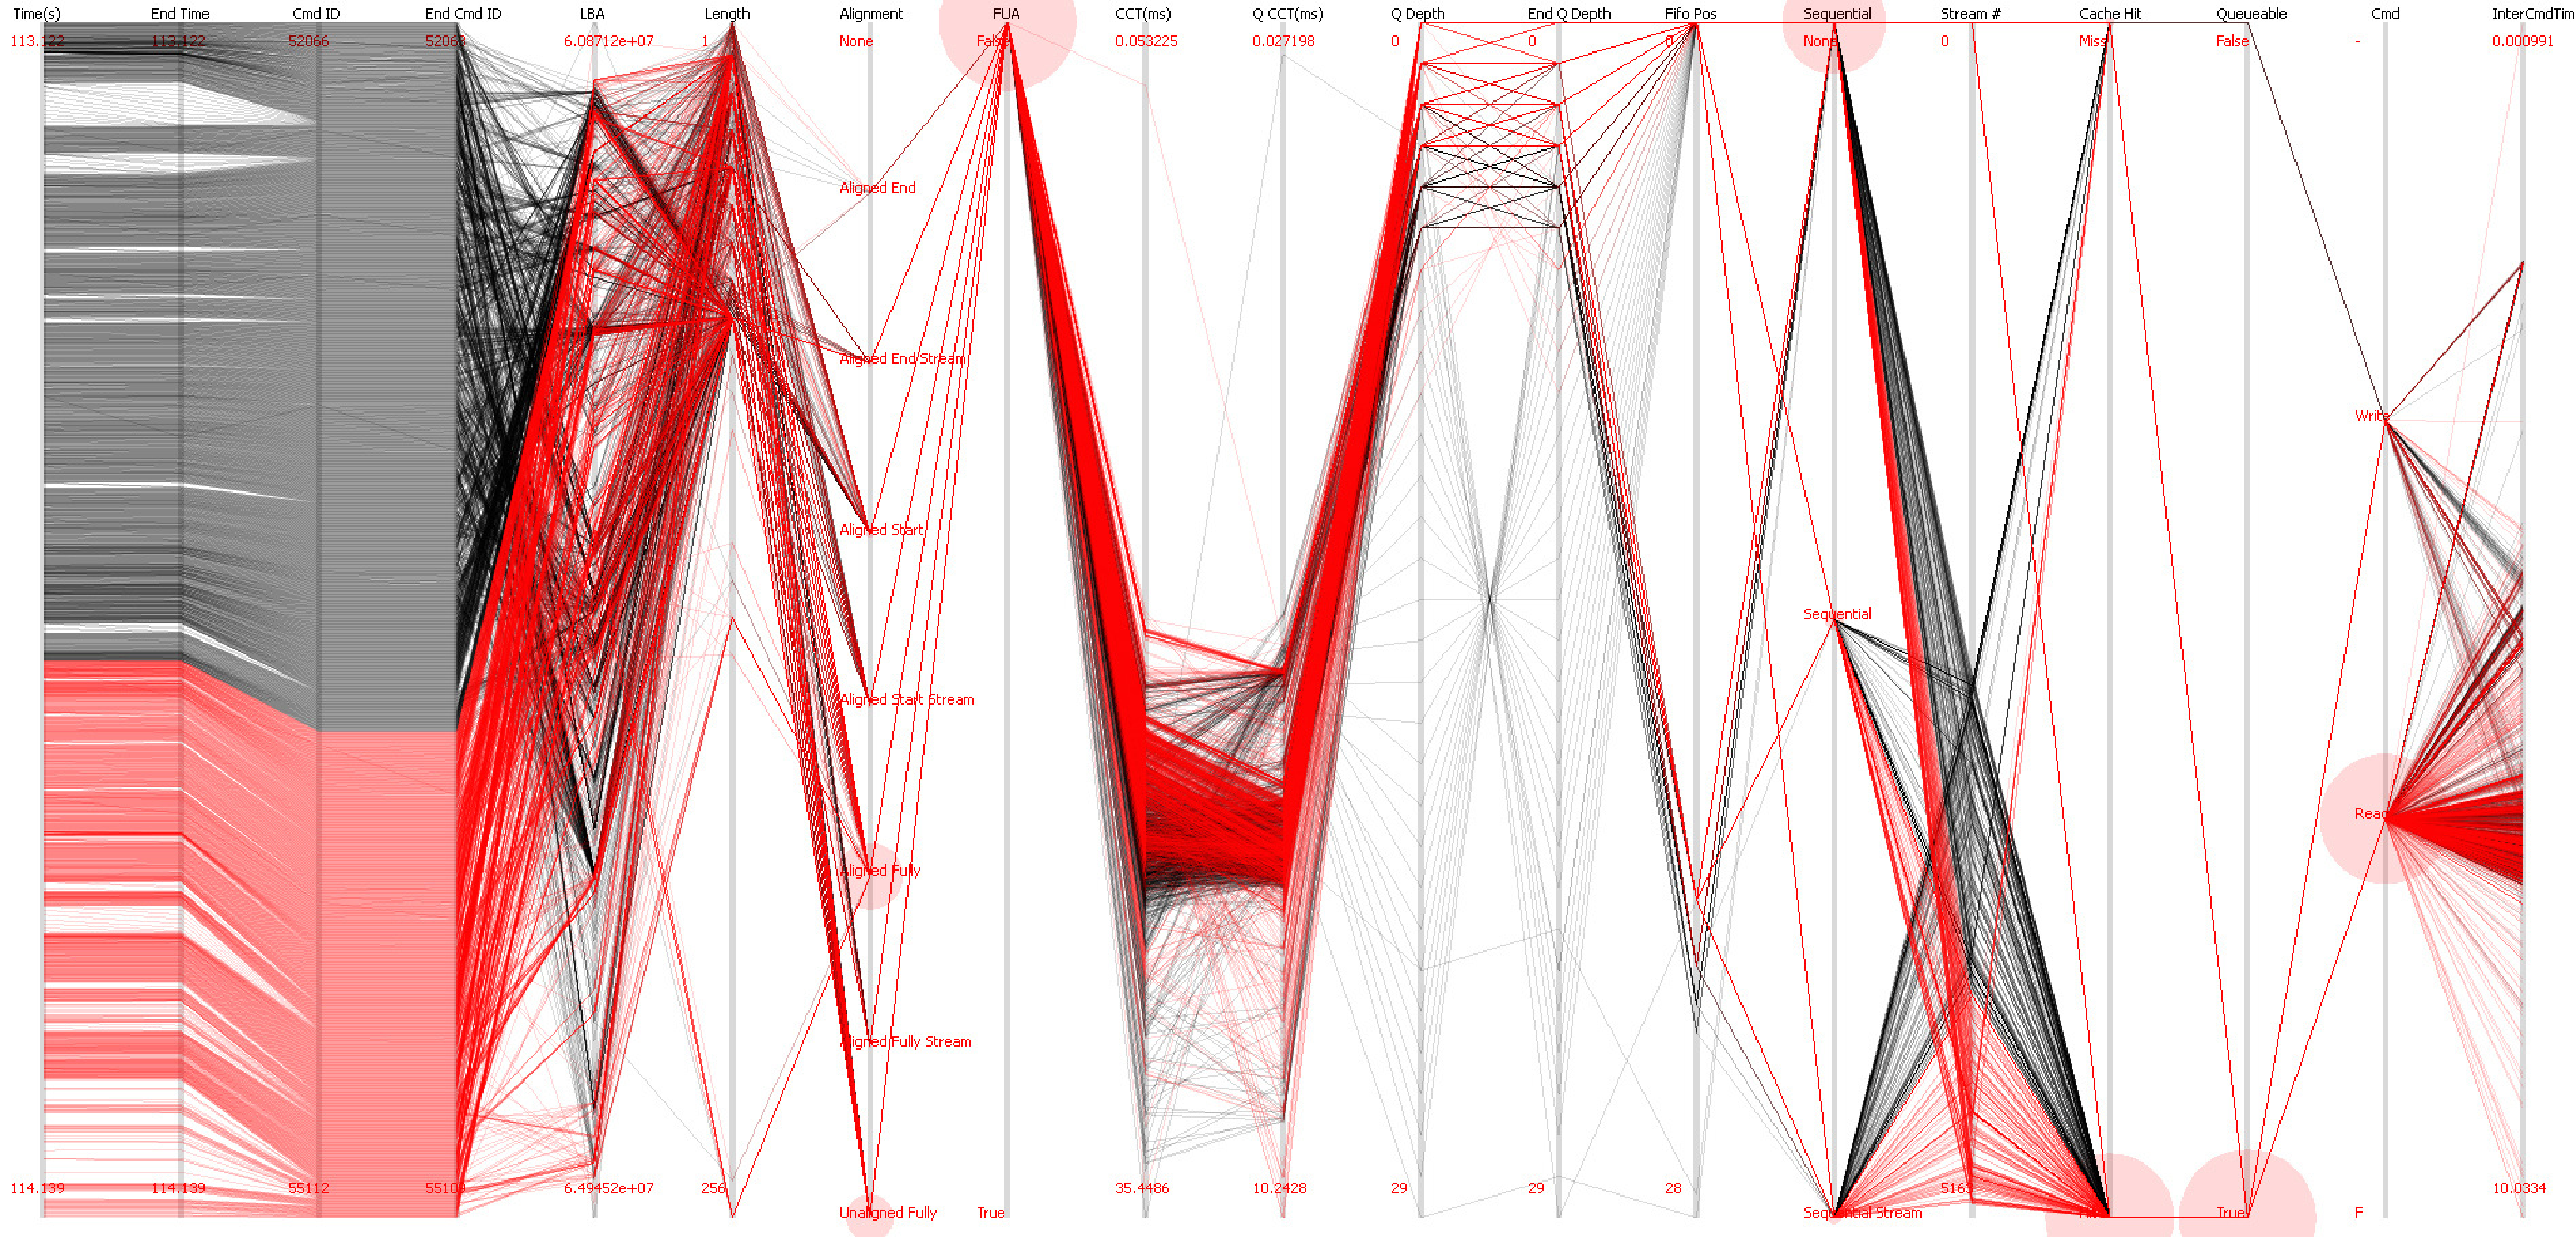
\includegraphics[width=\textwidth]{images/brush_focus5.pdf}
 \caption[Applying brushing to a range of commands in the dataset.]{Focusing on a particular range of data and applying brushing to a range of commands.}
 \label{fig:brush}
\end{figure}

\begin{figure}[h!]
 \centering
 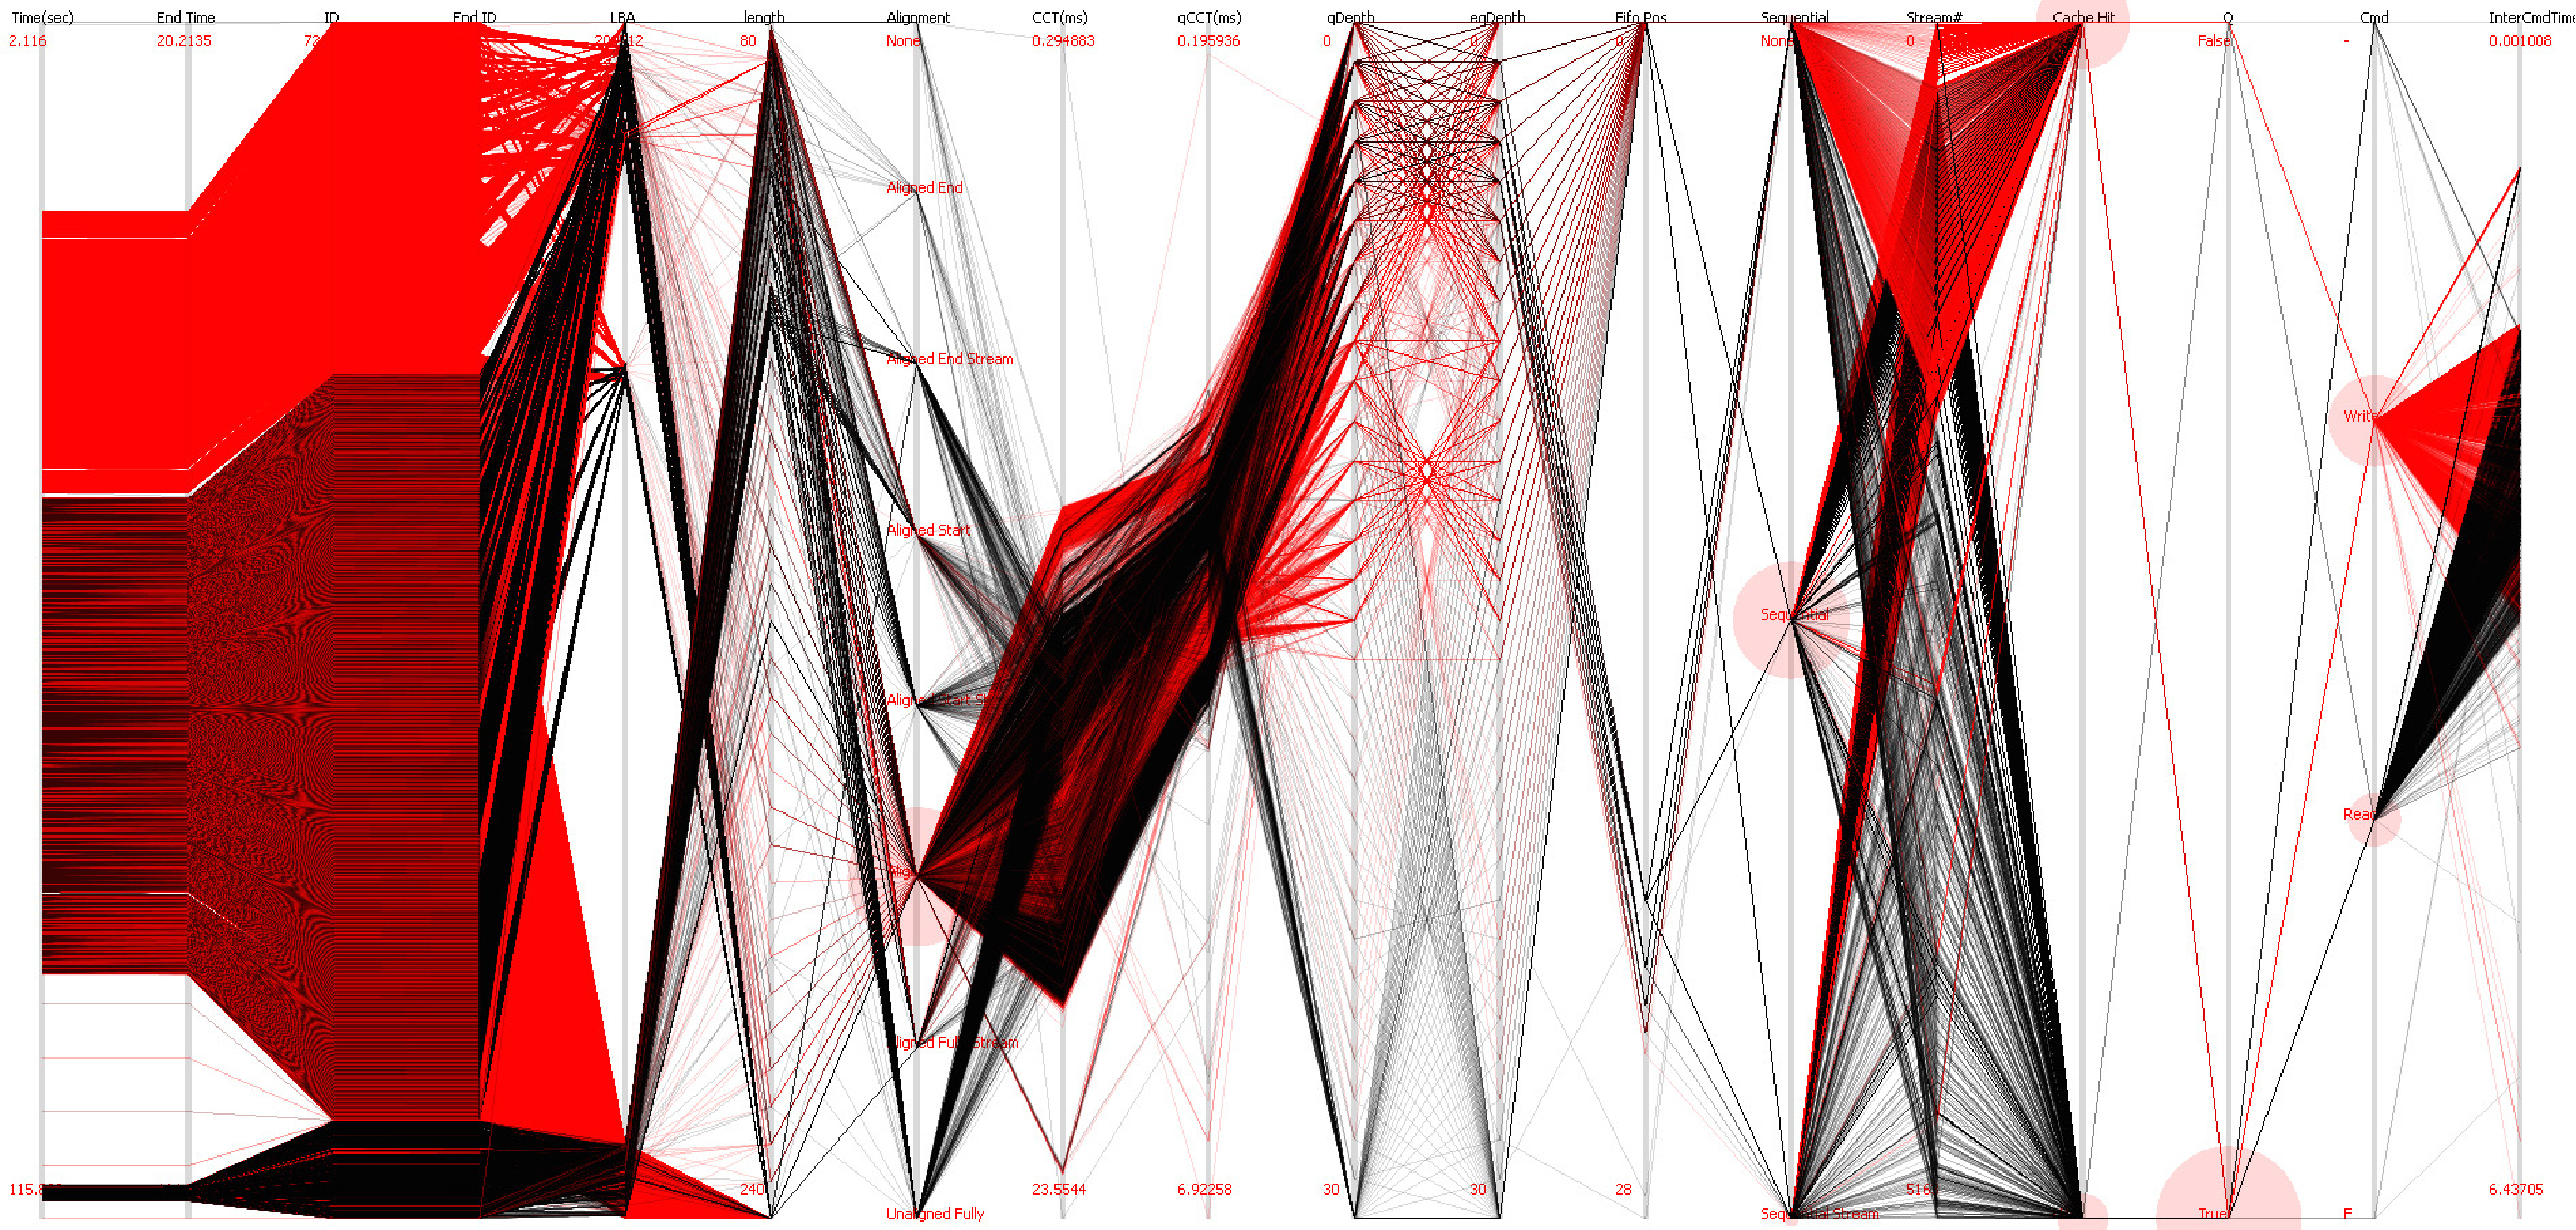
\includegraphics[width=\textwidth]{images/demo.pdf}
 \caption[Storage system workload dataset with write commands brushed.]{Overview of a storage system workload dataset with all write commands brushed.}
 \label{fig:brush2}
\end{figure}

\clearpage

\subsubsection{Focus}
Users can apply a focus on the dataset, which crops out all command values outside of the specified range. Applying a focus allows users to examine a smaller, often more manageable subset of data in order to observe occurrences specific to this particular data storage domain, such as interleaved threads and LBA banding. In Figure \ref{fig:focus_interleaving}, focusing on a smaller subset of Command ID values and eliminating other axes besides Command ID and LBA clearly exposes thread interleaving, which will be a method of verifying our algorithm for identifying threads in our initial data preprocessing.

\begin{figure}[h!]
 \centering
 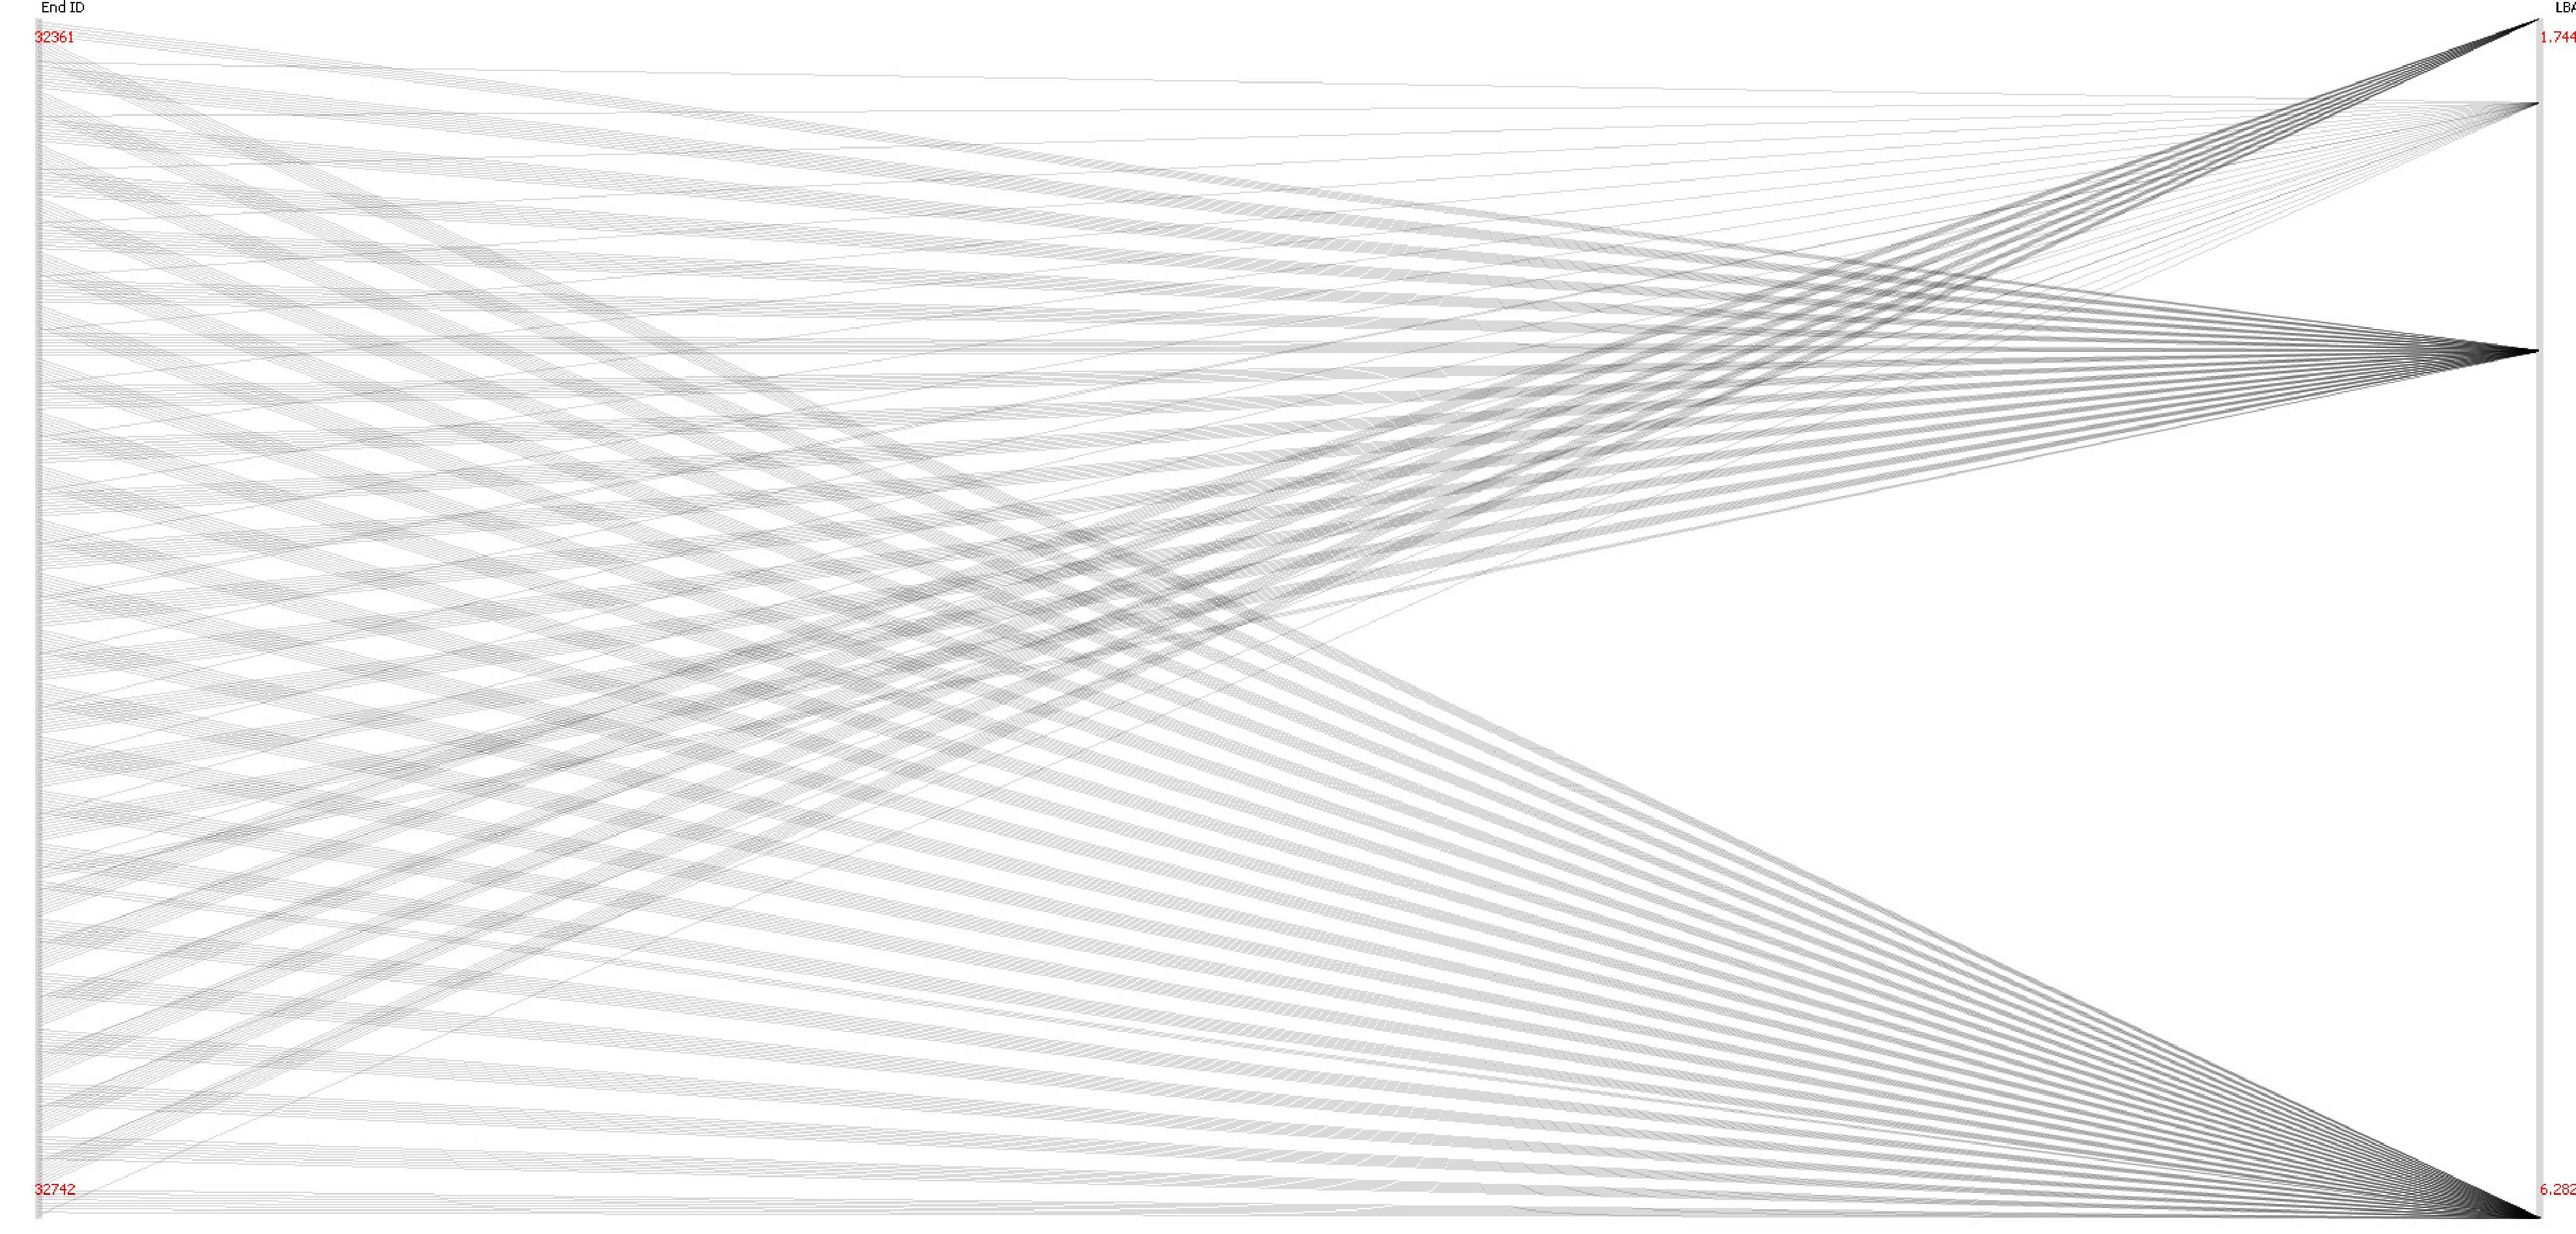
\includegraphics[width=\textwidth]{images/interleaved_bw.pdf}
 \caption[Thread interleaving observed by focusing on a range of data.]{Apparent thread interleaving observed by focusing on a particular range of data.}
 \label{fig:focus_interleaving}
\end{figure}

\section{Thread Coloring}
Data storage designers we consulted with expressed an interest in identifying interleaved threading, an occurrence where multiple running threads access the storage device in turn, which can lead to LBA banding. In order to illustrate interleaved threads, we implement an algorithm that identifies threads using predefined thresholds for LBA and number of commands. To preserve a visual distinction between threads, we assign a random color to each identified thread. Figure \ref{fig:color_overview} displays an overview of the full dataset with threads rendered in a color unique to the thread.

\begin{figure}[h!]
 \centering
 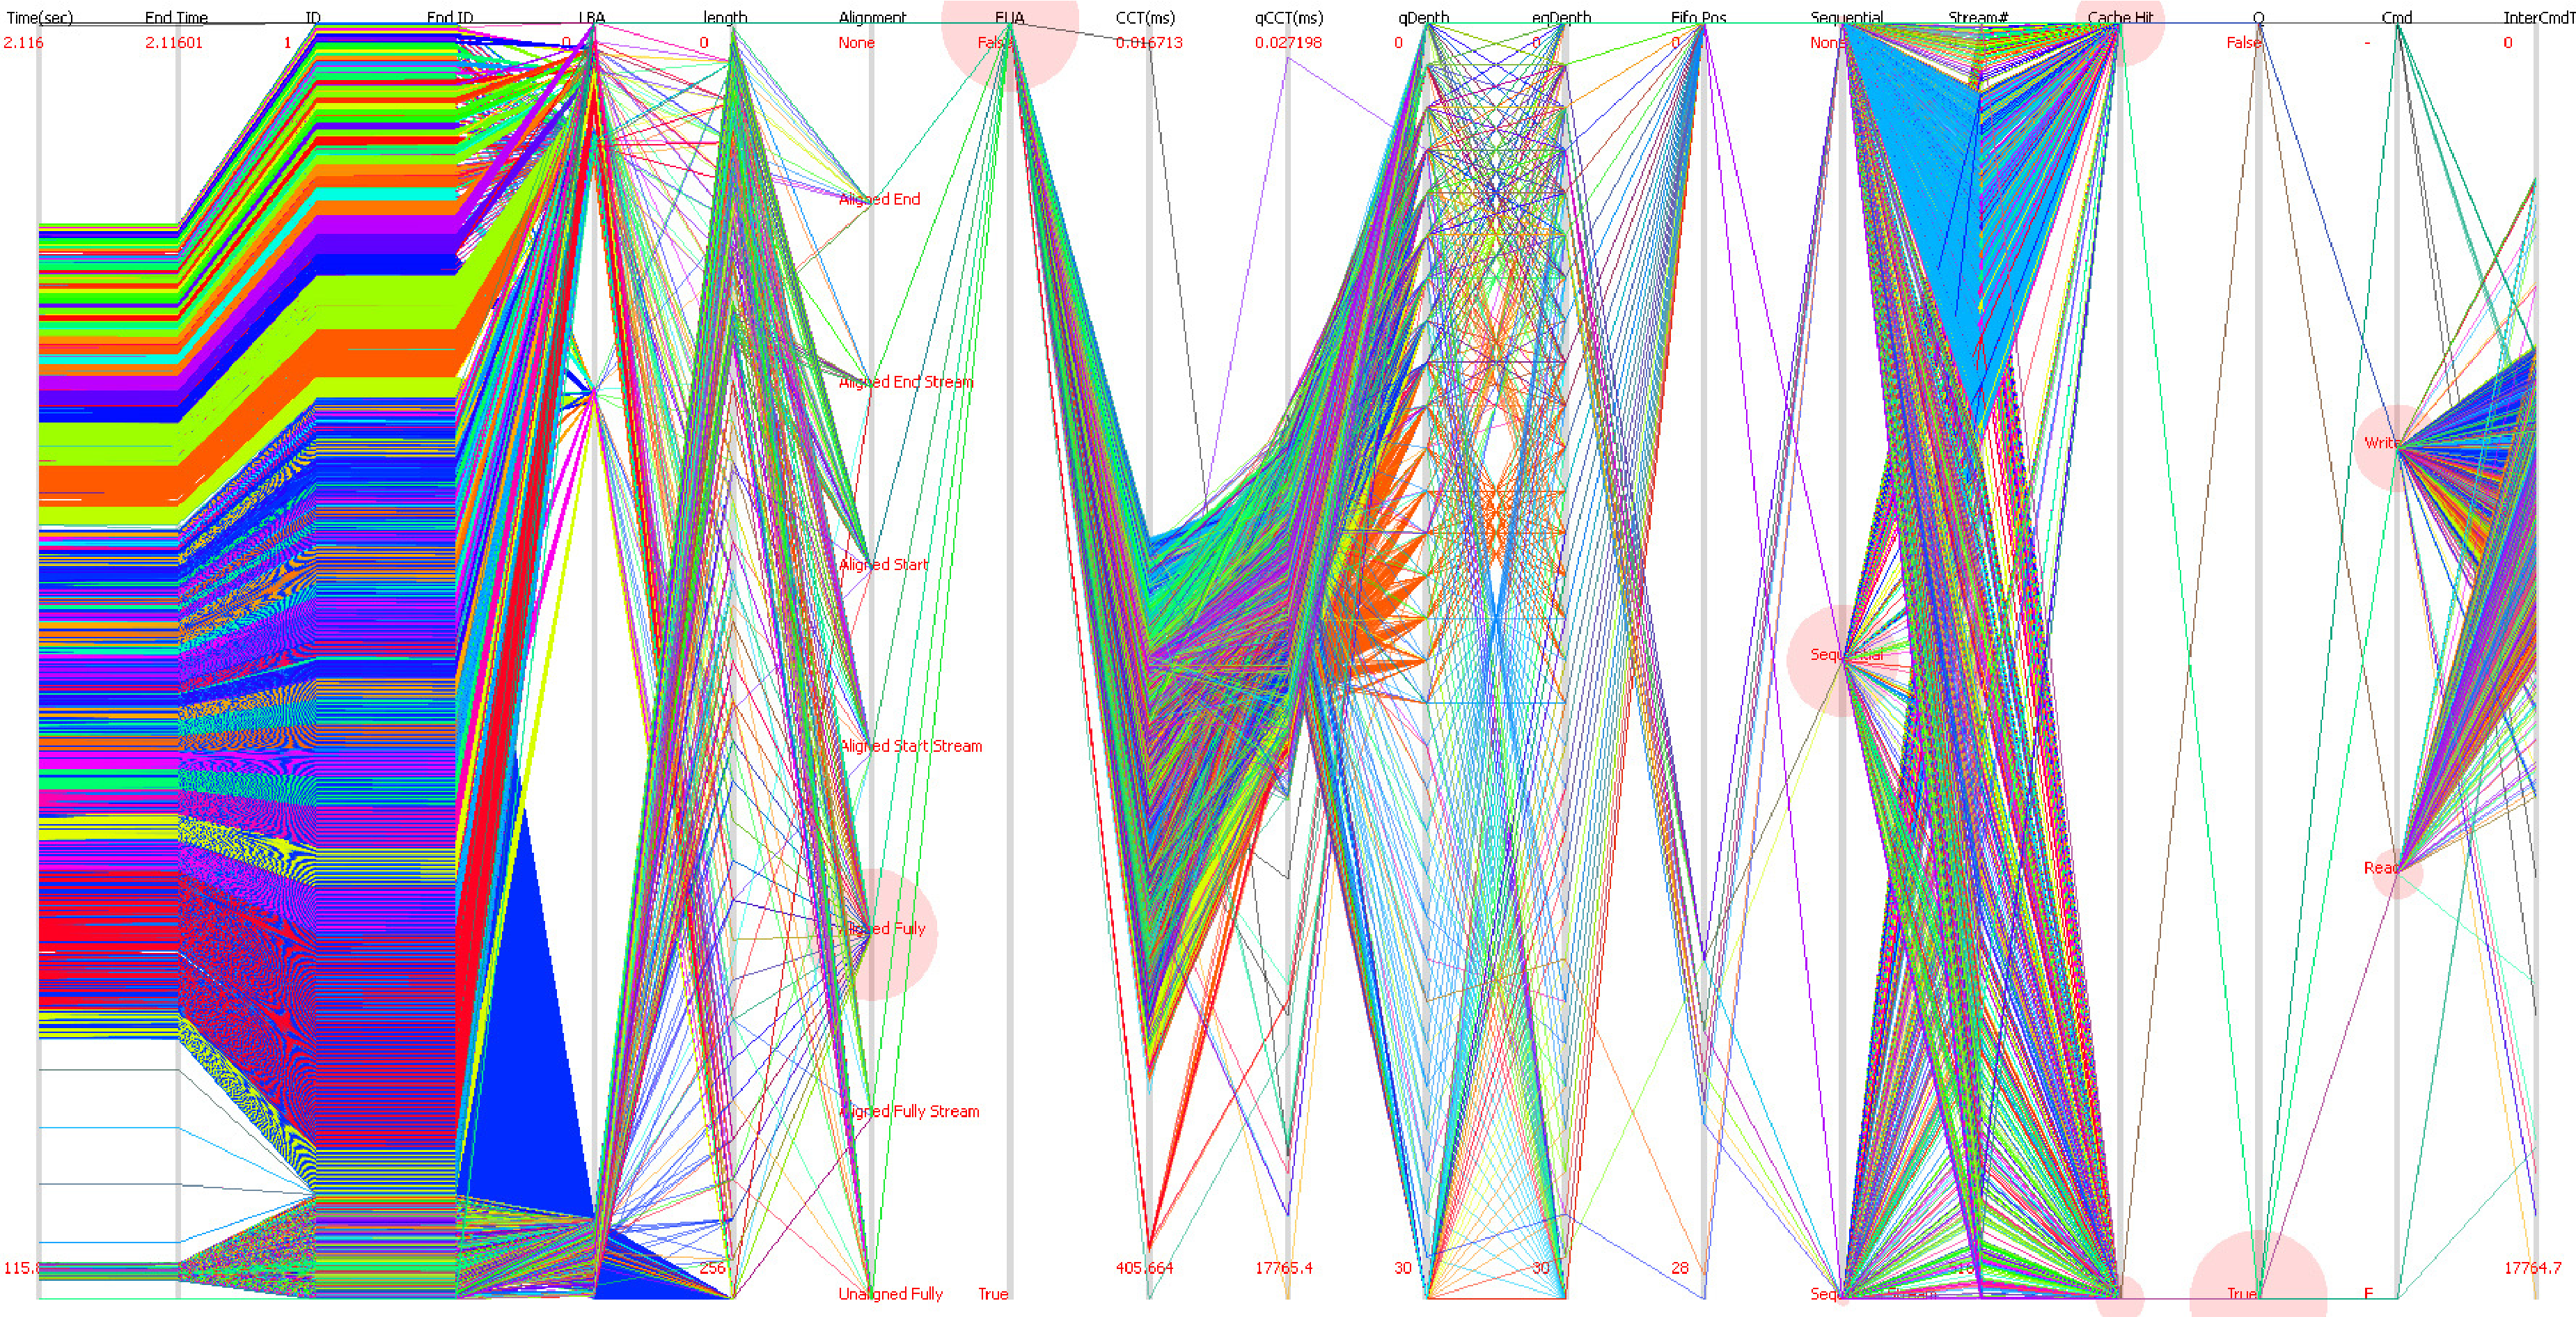
\includegraphics[width=\textwidth]{images/color_overview.pdf}
 \caption[Identified threads rendered with a thread exclusive color.]{Overview of a sample storage system workload dataset with each machine identified thread rendered with a thread exclusive color.}
 \label{fig:color_overview}
\end{figure}

\subsection{Thread Identification Algorithm}
We apply preprocessing to identify and assign unique colors to threads, using predefined thresholds for LBA and number of commands. The algorithm maintains a collection of recently identified threads, a default threshold (lba\_threshold) for LBAs, and a default threshold for numbers of command (command\_threshold). We iterate through each record in the dataset in the order they appear, and determine if they belong to a recently identified thread by calculating the lba\_delta, and maintaining a time\_to\_live variable for each thread, illustrated below:

\begin{algorithmic}
\FORALL{$record$ in $records$}
    % \STATE $thread\_iterator\gets recent\_threads.iterator$
    % \STATE $thread \gets thread\_iterator.next()$
    % \STATE $lba\_delta\gets |thread.lba - record.lba|$
    \STATE\COMMENT{Iterate through each thread in recent\_threads}
    \WHILE{$thread\_iterator.hasNext()$ \AND $lba\_delta > lba\_threshold$}
      \STATE $thread \gets thread\_iterator.next()$
      \STATE $lba\_delta\gets |thread.lba - record.lba|$
    \ENDWHILE

    % \FORALL{$thread$ in $recent\_threads$} \STATE\COMMENT{Decrement the time\_to\_live for all recent threads}
    %   \STATE $thread.time\_to\_live \gets thread.time\_to\_live - 1$
    % \ENDFOR

    \IF {$lba\_delta \leq lba\_threshold$} \STATE\COMMENT{This record belongs to a recently identified thread}
        \STATE $thread.lba \gets record.lba$
        \STATE $thread.time\_to\_live \gets command\_threshold$
    \ELSE \STATE\COMMENT{This record belongs to a new thread}
      \STATE $new\_thread.lba \gets record.lba$
      \STATE $new\_thread.time\_to\_live \gets command\_threshold$
      \STATE $new\_thread.color \gets generateNewColor()$
      \STATE $recent\_threads.insert(new\_thread) $
    \ENDIF

    \STATE {Decrement the time\_to\_live for all recent threads, remove threads from recent\_threads once the time\_to\_live value is zero}

\ENDFOR
\end{algorithmic}

We suggest the use of thread coloring in conjunction with a user specified focus and beginning with a view showing only the Command ID and LBA axes to observe thread interleaving. An example of this combination of features is illustrated in Figure \ref{fig:color_focus1}. In this particular screen capture, we can observe a long-running thread colored yellow, which interleaves with the various other threads colored with hues of red, green, and blue. Applying a focus on a smaller subset of the same data, Figure \ref{fig:color_focus2} displays the thread interleaving more clearly, with each thread performing a few accesses before trading off with another thread.

\begin{figure}[h!]
 \centering
 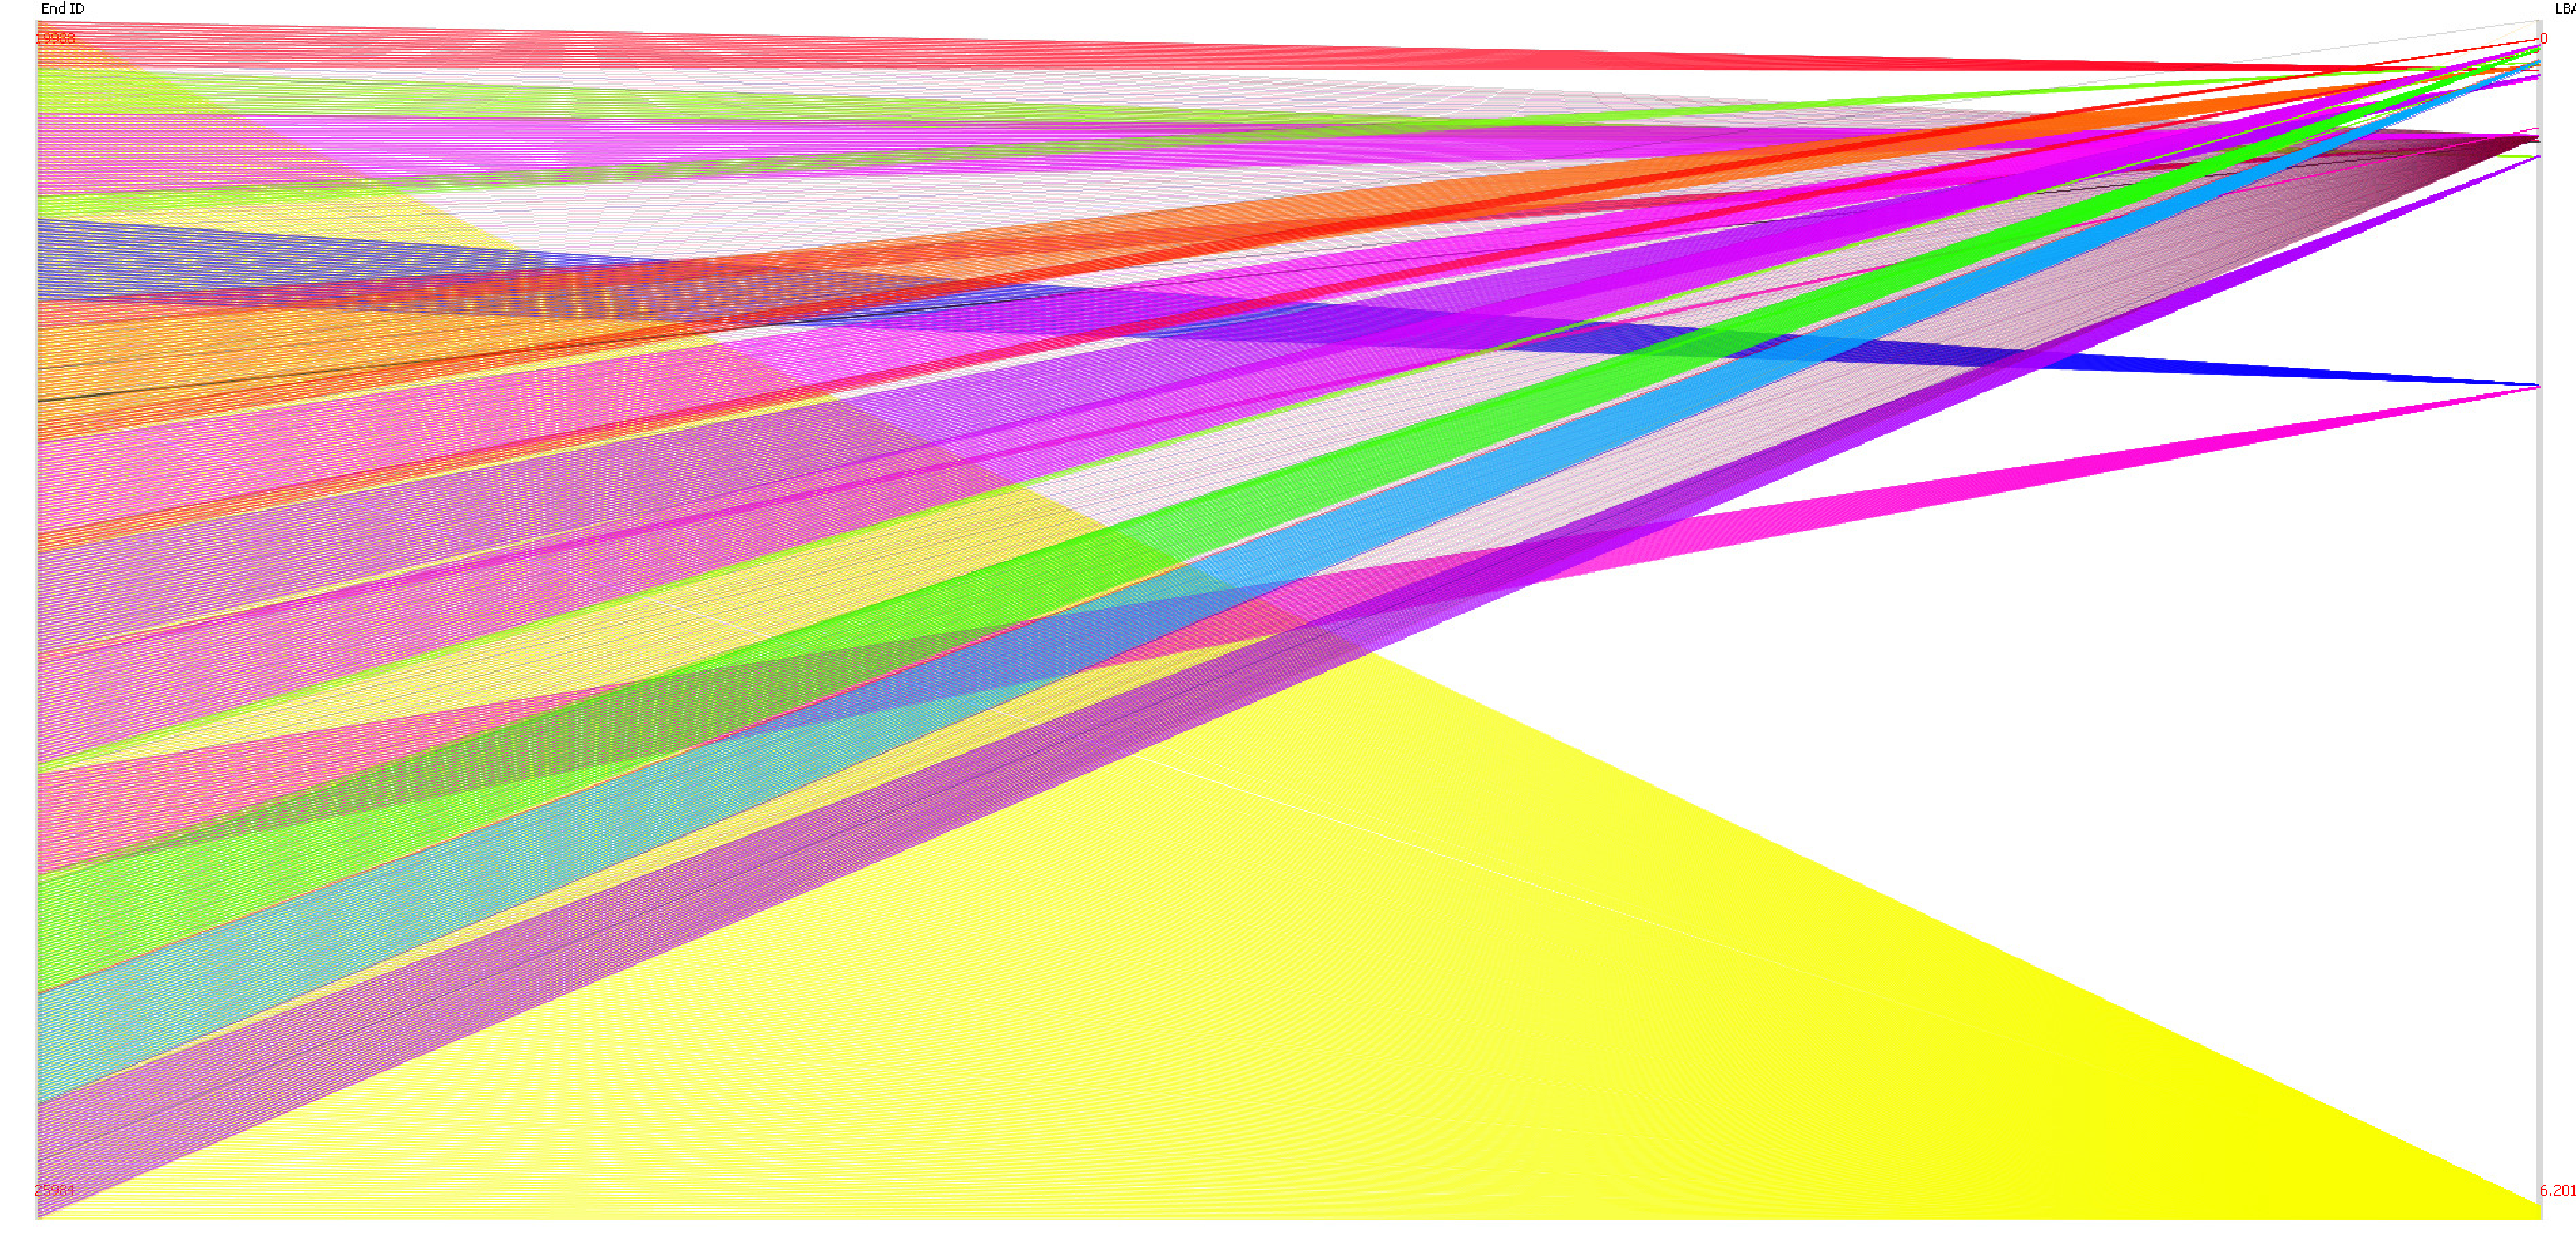
\includegraphics[width=\textwidth]{images/interleaved_color2.pdf}
 \caption[Identified threads rendered with a thread exclusive color.]{Interleaved threads conveyed by illustrating each machine identified thread with a thread exclusive color.}
 \label{fig:color_focus1}
\end{figure}

\begin{figure}[h!]
 \centering
 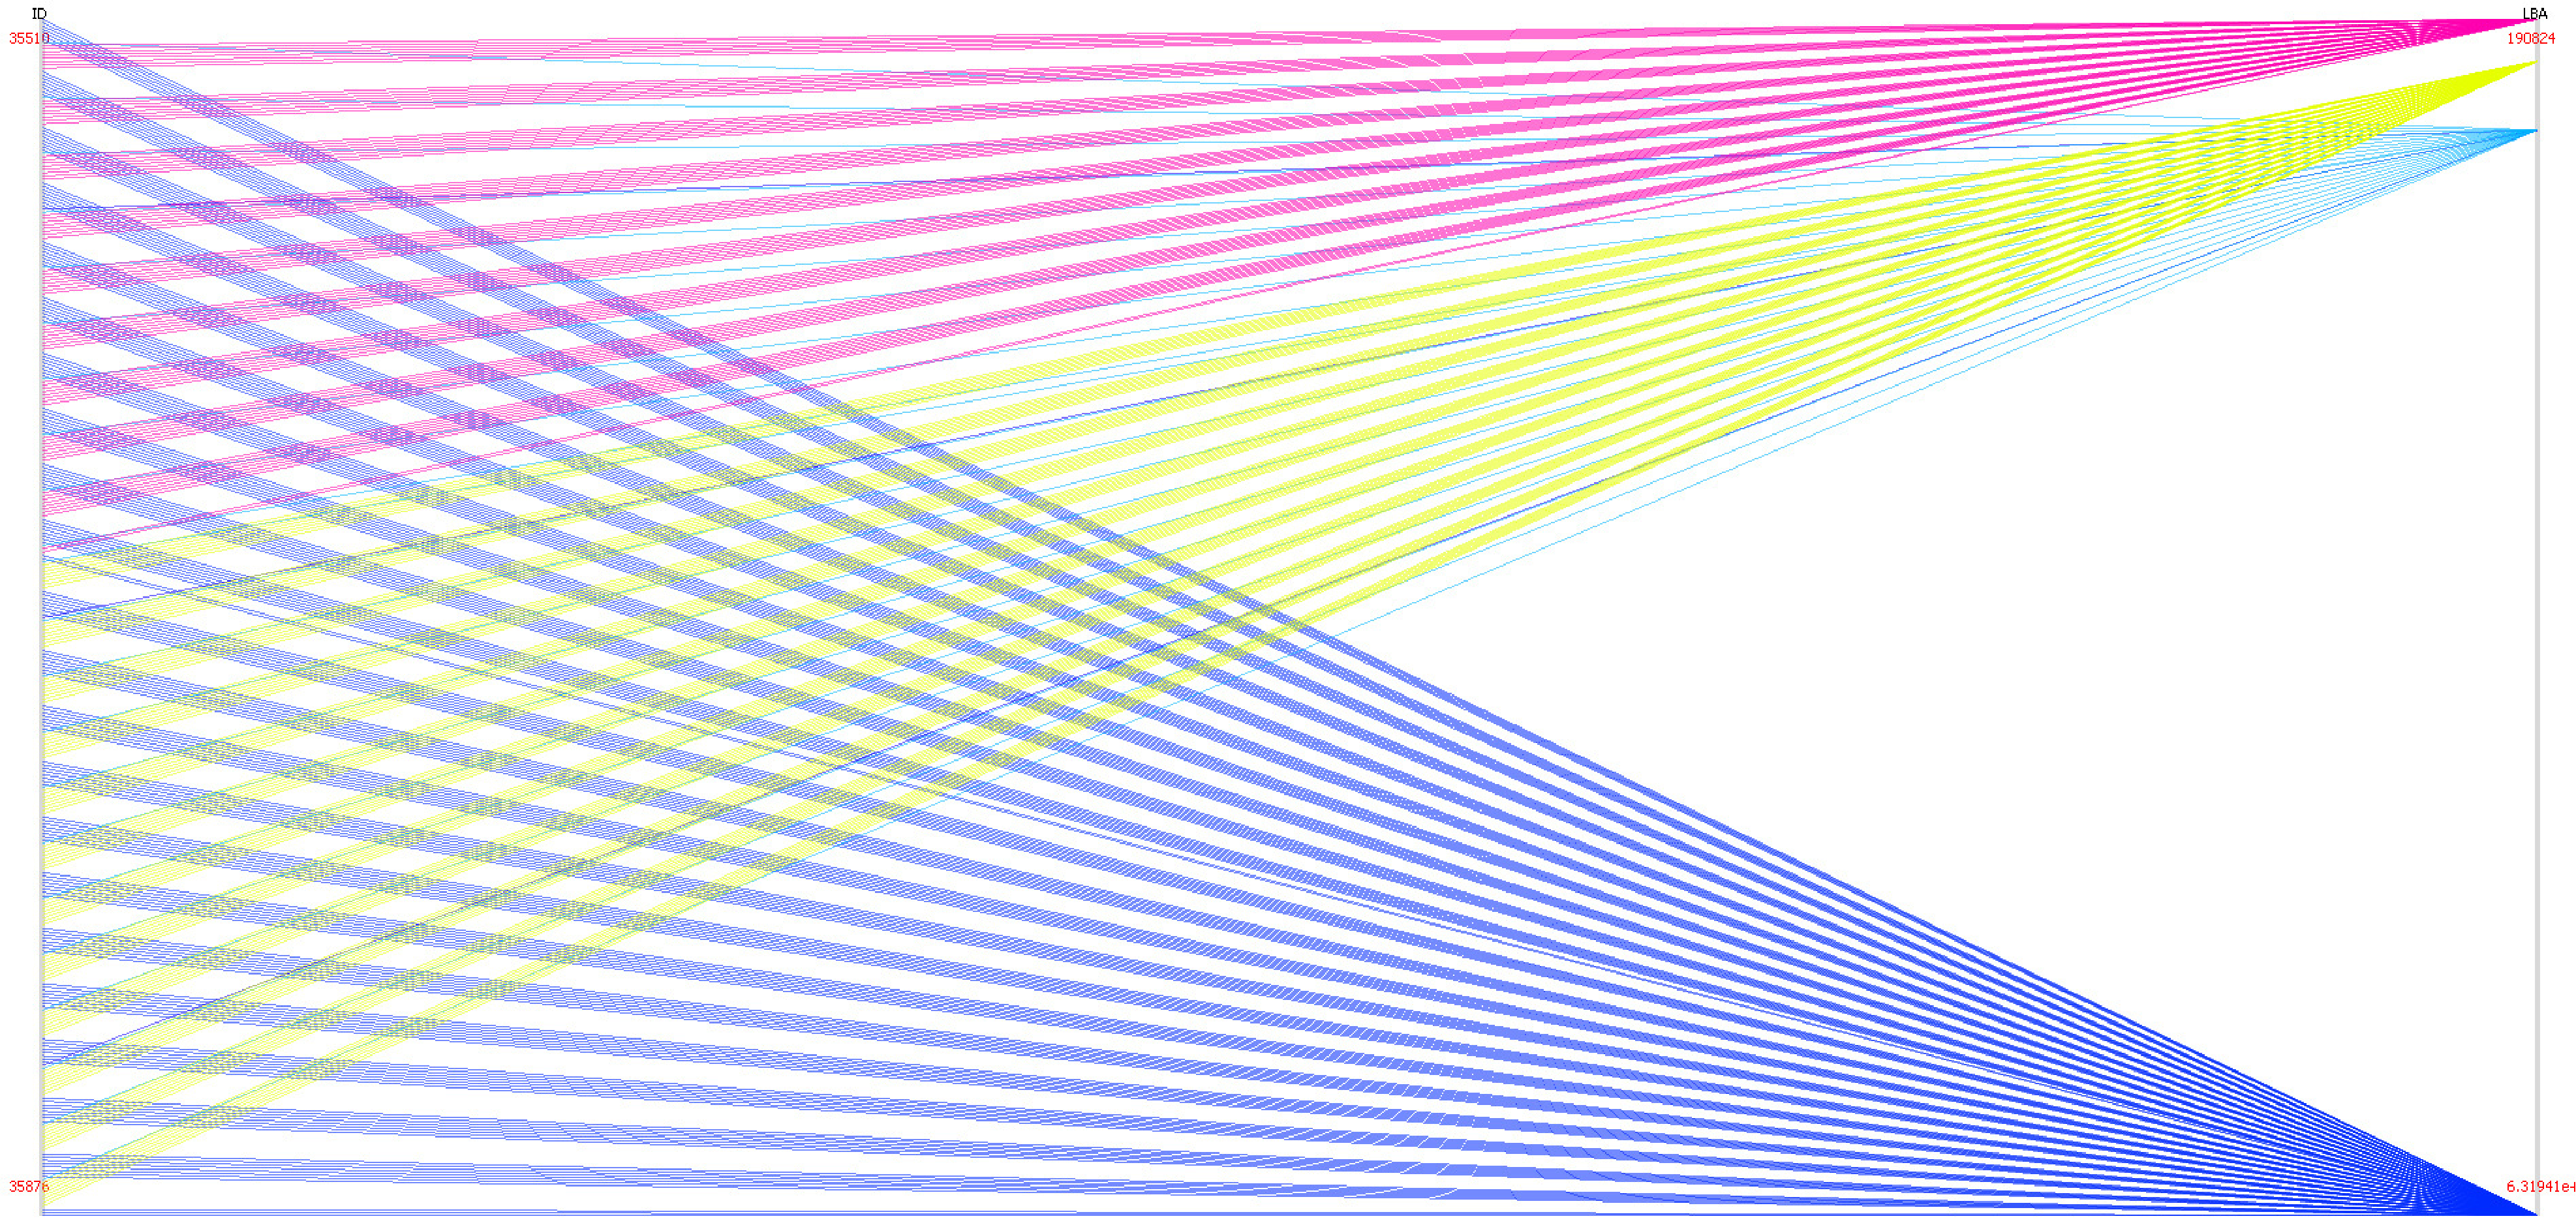
\includegraphics[width=\textwidth]{images/interleaved_color4.pdf}
 \caption[A subset of data rendered with a thread exclusive colors.]{Focusing on a smaller subset of data more clearly displays interleaved threads, conveyed by illustrating each machine identified thread with a thread exclusive color.}
 \label{fig:color_focus2}
\end{figure}

\subsection{Unique Color Generation}
Unique colors are generated by manipulating Hue Saturation Brightness (HSB) values, setting saturation and brightness as maximum constants, and incorporating a random number generator to determine hue. Applying this method ensures that each thread will be a different color that is relatively distinguishable from others without the need to consider differing levels of saturation and brightness for the same hue values. 

Random numbers are generated with a hard coded seed, ensuring that each usage of the tool assigns the same colors for each thread across multiple runs of the tool.

\section{Implementation}

\subsection{Languages and Frameworks}
This visualization tool was written in C++, OpenGL, and utilizing the Qt framework. Our tool uses Qt because it is a mature and widely used framework for developing applications for both Microsoft Windows and Linux operating systems~\cite{qt:nokia}. Support for these platforms is necessary for the industry of data storage systems, our primary intended users.

\subsection{Data Preprocessing}
Our tool reads input data from a CSV file, generated from a bus analyzer trace interpreter tool. We parse through this data and store them in memory using common data structures such as vectors, implemented in Qt in order to leverage the efficiency and abstractions created in their actively developed framework. 

\subsection{Rendering}
Accesses currently in view with respect to the user's manipulations are iteratively rendered by traversing the vector of data. User manipulations are implemented with transformation variables, describing the range of focus data, range of brushing, value of scaling, and values of two dimensional transition. This is currently a single-threaded process, however we acknowledge the future performance improvements and usability methods possible with exploring multi-threaded rendering implementation.

\subsection{Usability}
Most functionality is presented to the user through context menus, as shown in Figure \ref{fig:context_menus}. Here we can see the context menu for the End Time axis, providing the user with options to remove the dimension from the visualization, apply a brush to a range of data, create a focus on a selected range of data, or set the equation of the axis scale for this particular dimension. Although this is not ideal for certain operations such as rearranging axes, it serves as a relatively intuitive method to interact and manipulate parallel coordinates axes through the use of a computer mouse and keyboard.

\begin{figure}[h!]
 \centering
 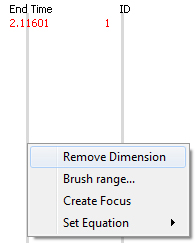
\includegraphics[width=0.5\textwidth]{images/context_menu.jpg}
 \caption[Context menus to interact with and manipulate axes.]{The use of context menus to interact with and manipulate parallel coordinates axes.}
 \label{fig:context_menus}
\end{figure}

Defining ranges of data is accomplished through the use of sliders and optional input fields, in order to provide the user with both coarse and fine-grained methods. Figure \ref{fig:sliders_input} is an example of the usage of sliders and input fields to select a range to brush the range of data to analyze and differentiate, allowing the user to utilize the sliders for coarse values, and the input fields for more specific values. Means of transformations are optimized again for mouse input, allowing translations through clicking and dragging the visualization, and scaling using a slider at the bottom of the application window.

\begin{figure}[h!]
 \centering
 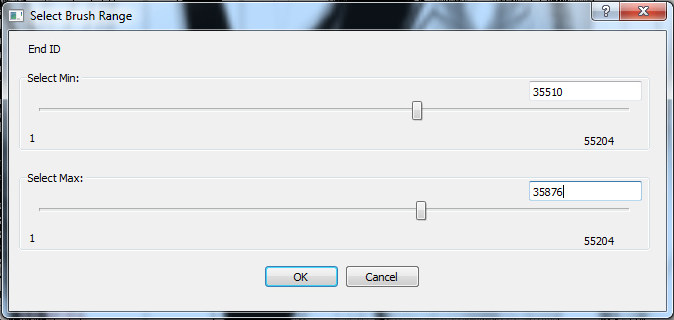
\includegraphics[width=\textwidth]{images/select_range.jpg}
 \caption[Sliders and input fields for specifying ranges of data.]{The use of sliders and input fields to provide coarse and fine-grain methods for specifying ranges of data.}
 \label{fig:sliders_input}
\end{figure}


\chapter{Results}
\label{results}

We analyzed various storage system captures with our tool, including corporate production workloads. We then conducted a user study that assisted in identifying areas of our visualization that were effective in comparison to tools currently used, and areas which need improvement to better serve our users.

\section{Images}
We present the following figures, which illustrate our tool and the various datasets analyzed.

\begin{figure}[h!]
 \centering
 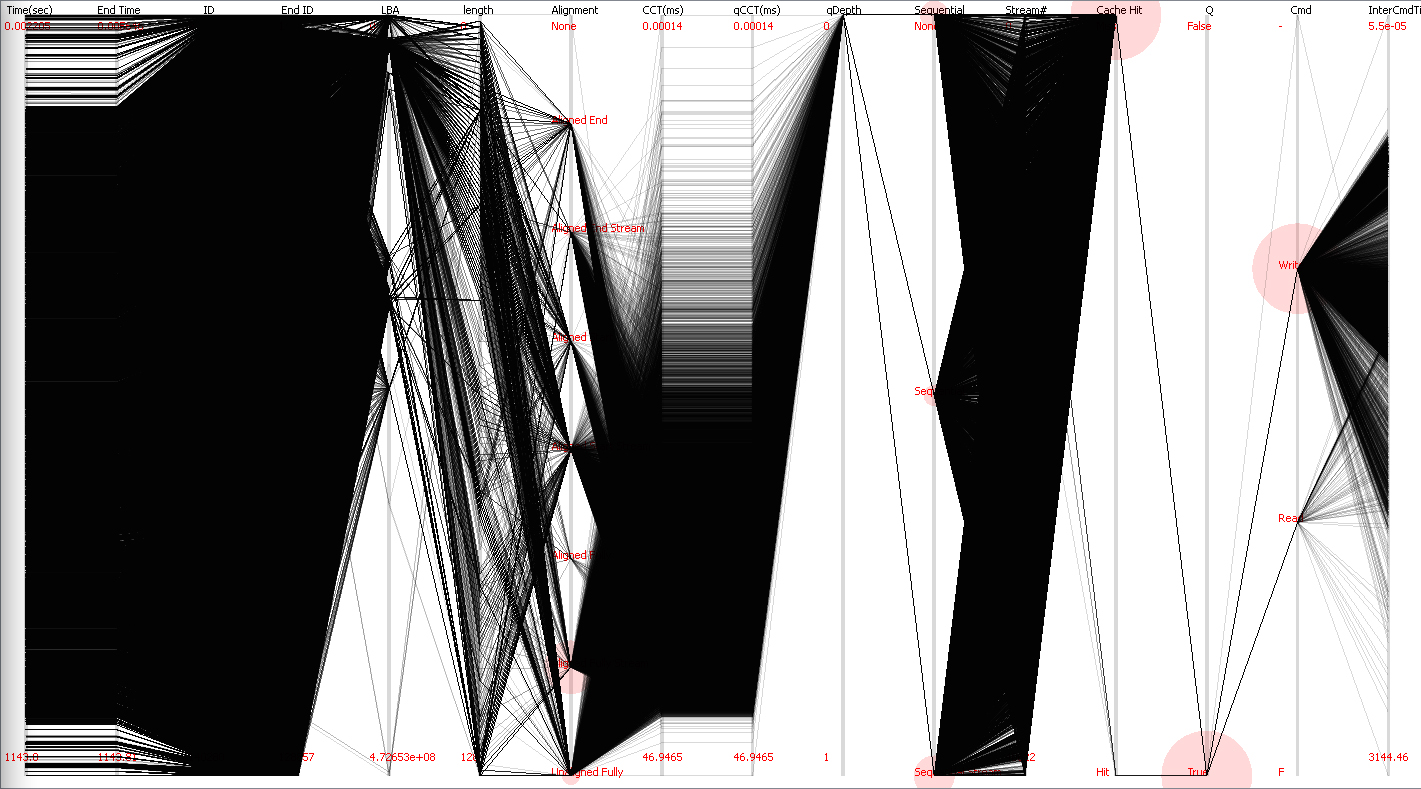
\includegraphics[width=\textwidth]{images/1.jpg}
 \caption[Production workload obtained from a partner corporation.]{Overview of a production storage system workload captured dataset obtained from a partner corporation.}
\end{figure}

\begin{figure}[h!]
 \centering
 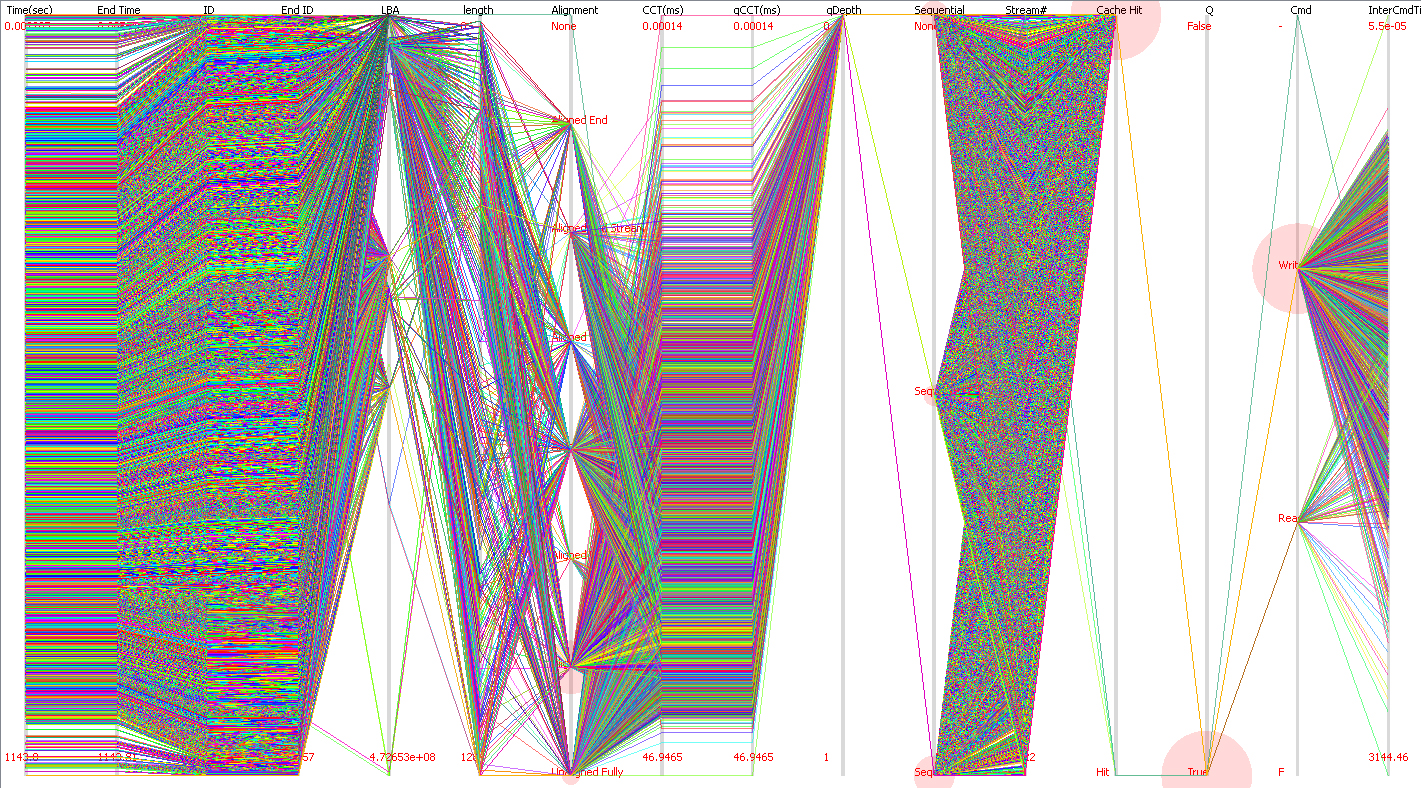
\includegraphics[width=\textwidth]{images/2.jpg}
 \caption[Production workload with threads colored.]{Overview of a production storage system workload captured dataset obtained from a partner corporation with identified threads colored.}
\end{figure}

\begin{figure}[h!]
 \centering
 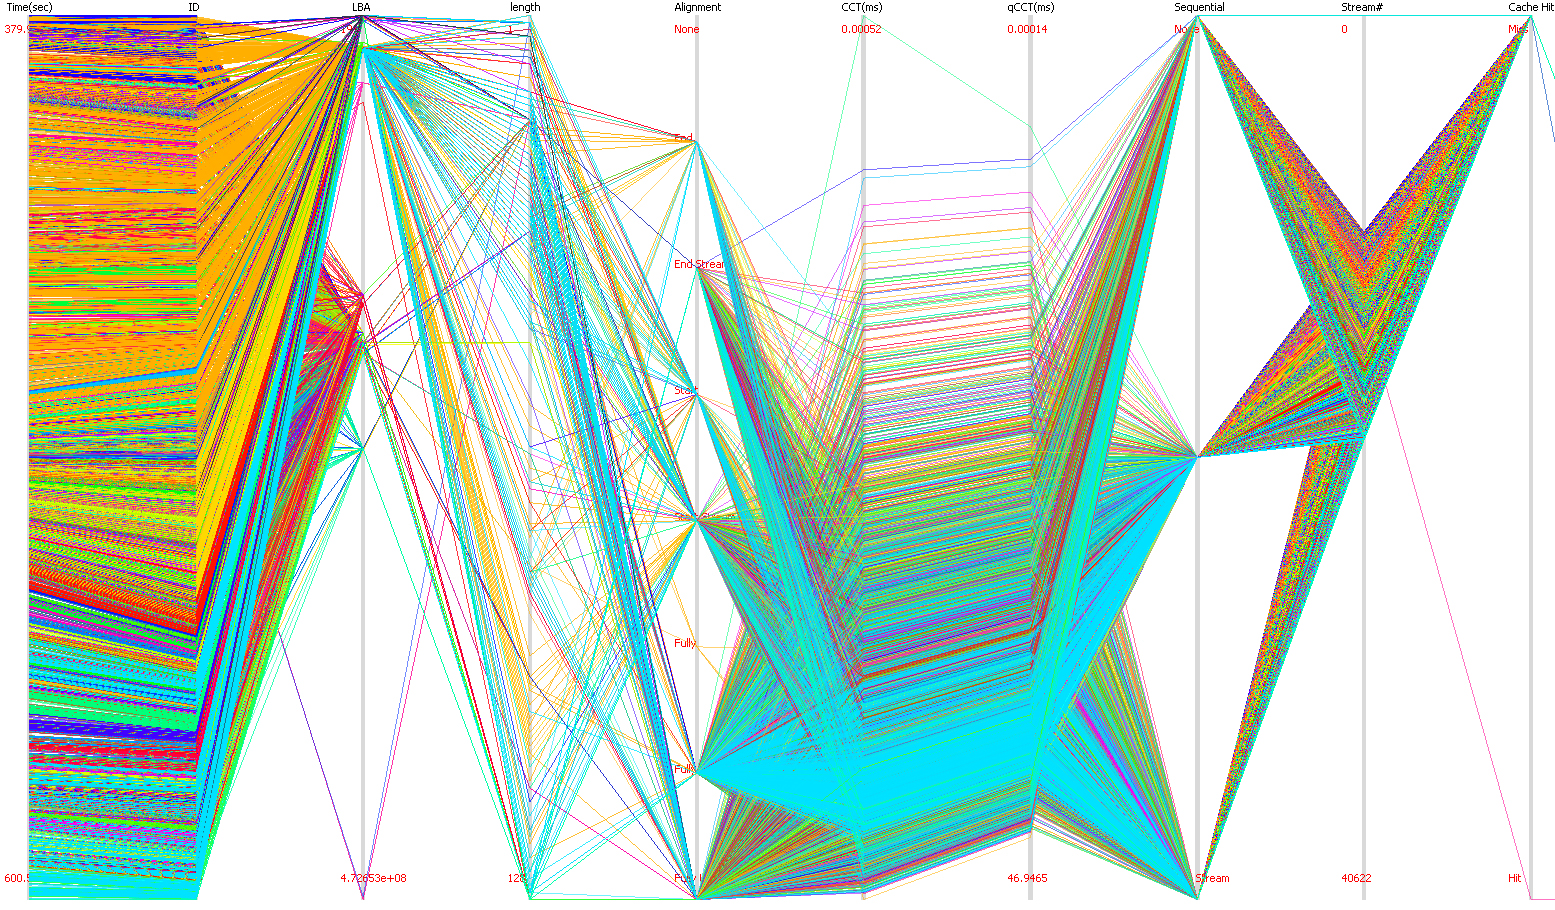
\includegraphics[width=\textwidth]{images/3.jpg}
 \caption[Focus on a production workload with threads colored.]{A production storage system workload captured dataset obtained from a partner corporation with identified threads coloring, axes rearrangement, and a subset focus applied.}
\end{figure}

\begin{figure}[h!]
 \centering
 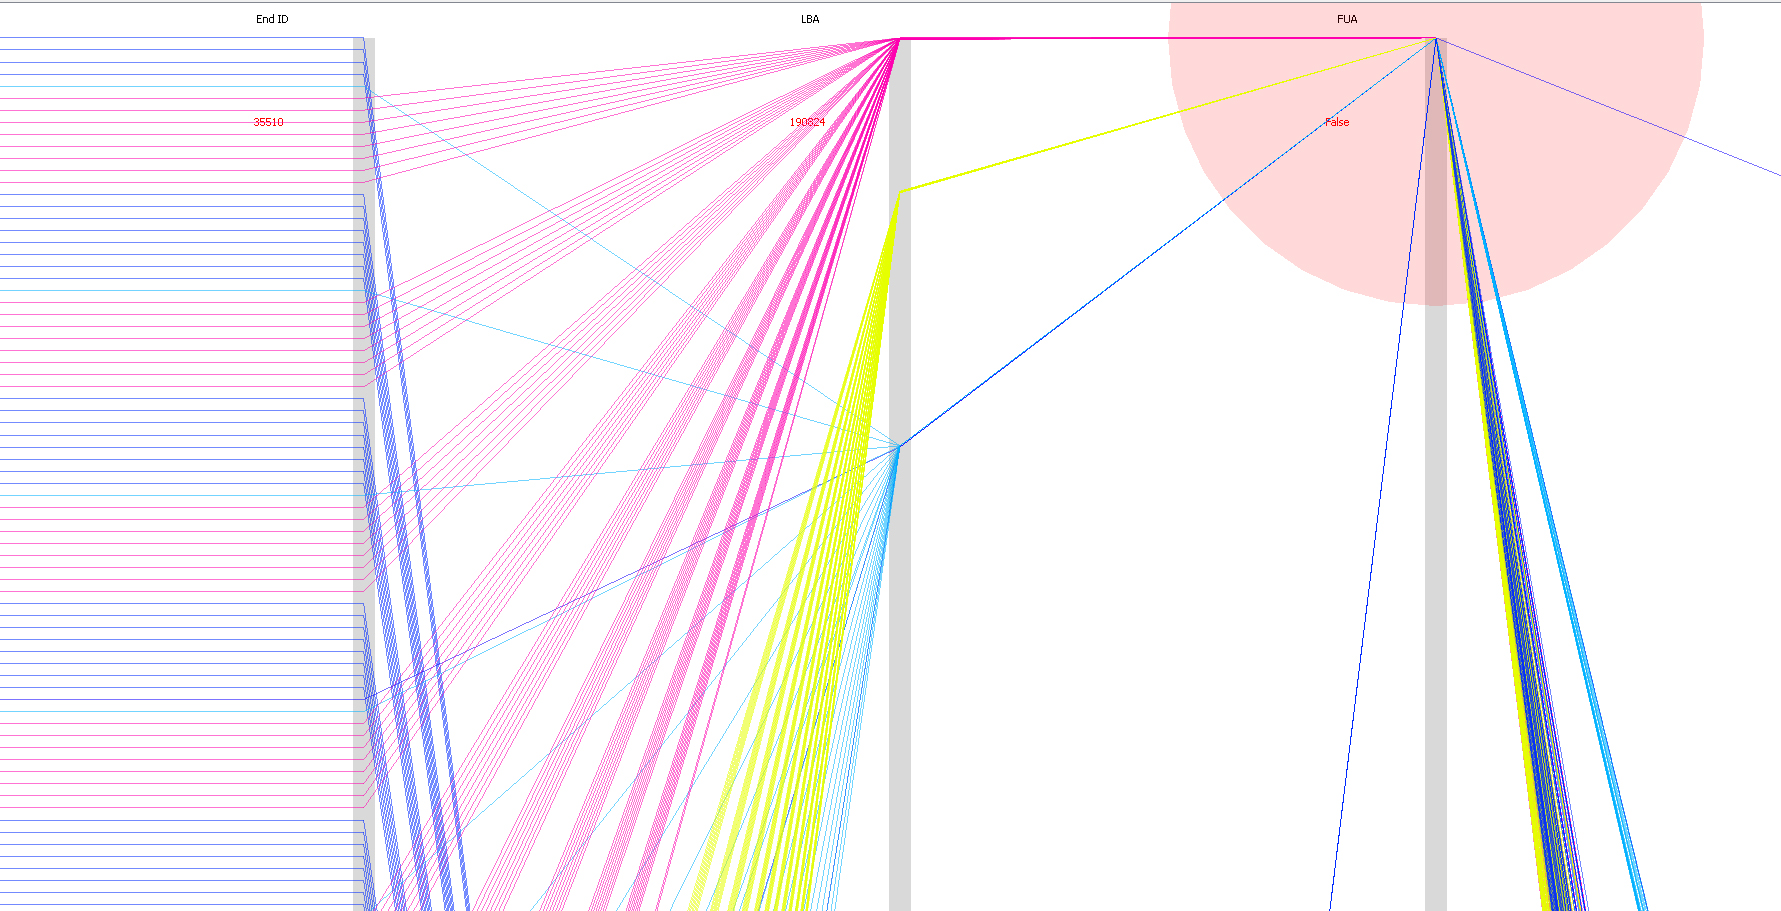
\includegraphics[width=\textwidth]{images/4.jpg}
 \caption[Focus applied on a production workload with threads colored.]{A production storage system workload captured dataset obtained from a partner corporation with identified threads coloring, axes rearrangement, a subset focus, and inward scaling applied.}
\end{figure}

\begin{figure}[h!]
 \centering
 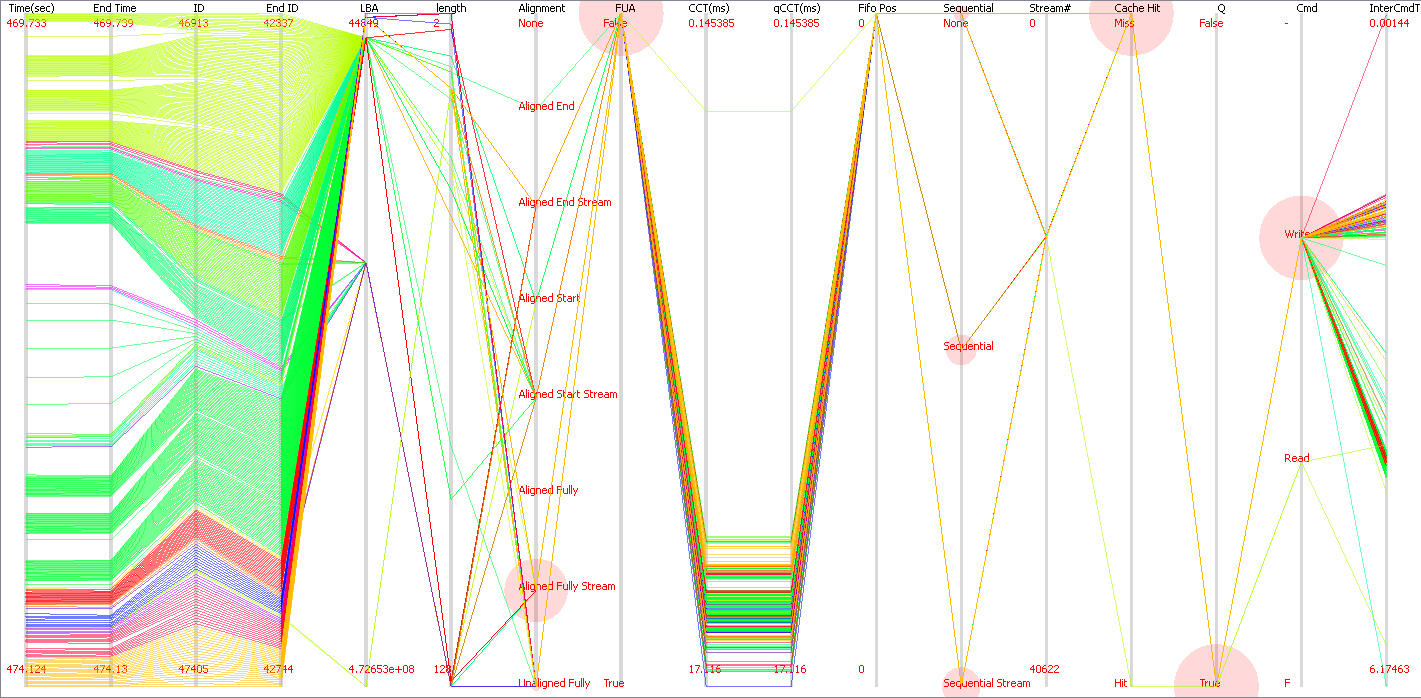
\includegraphics[width=\textwidth]{images/5.jpg}
 \caption[Focus applied on a production workload with threads colored.]{A production storage system workload captured dataset obtained from a partner corporation with identified threads coloring, axes rearrangement, and a subset focus applied.}
\end{figure}

\begin{figure}[h!]
 \centering
 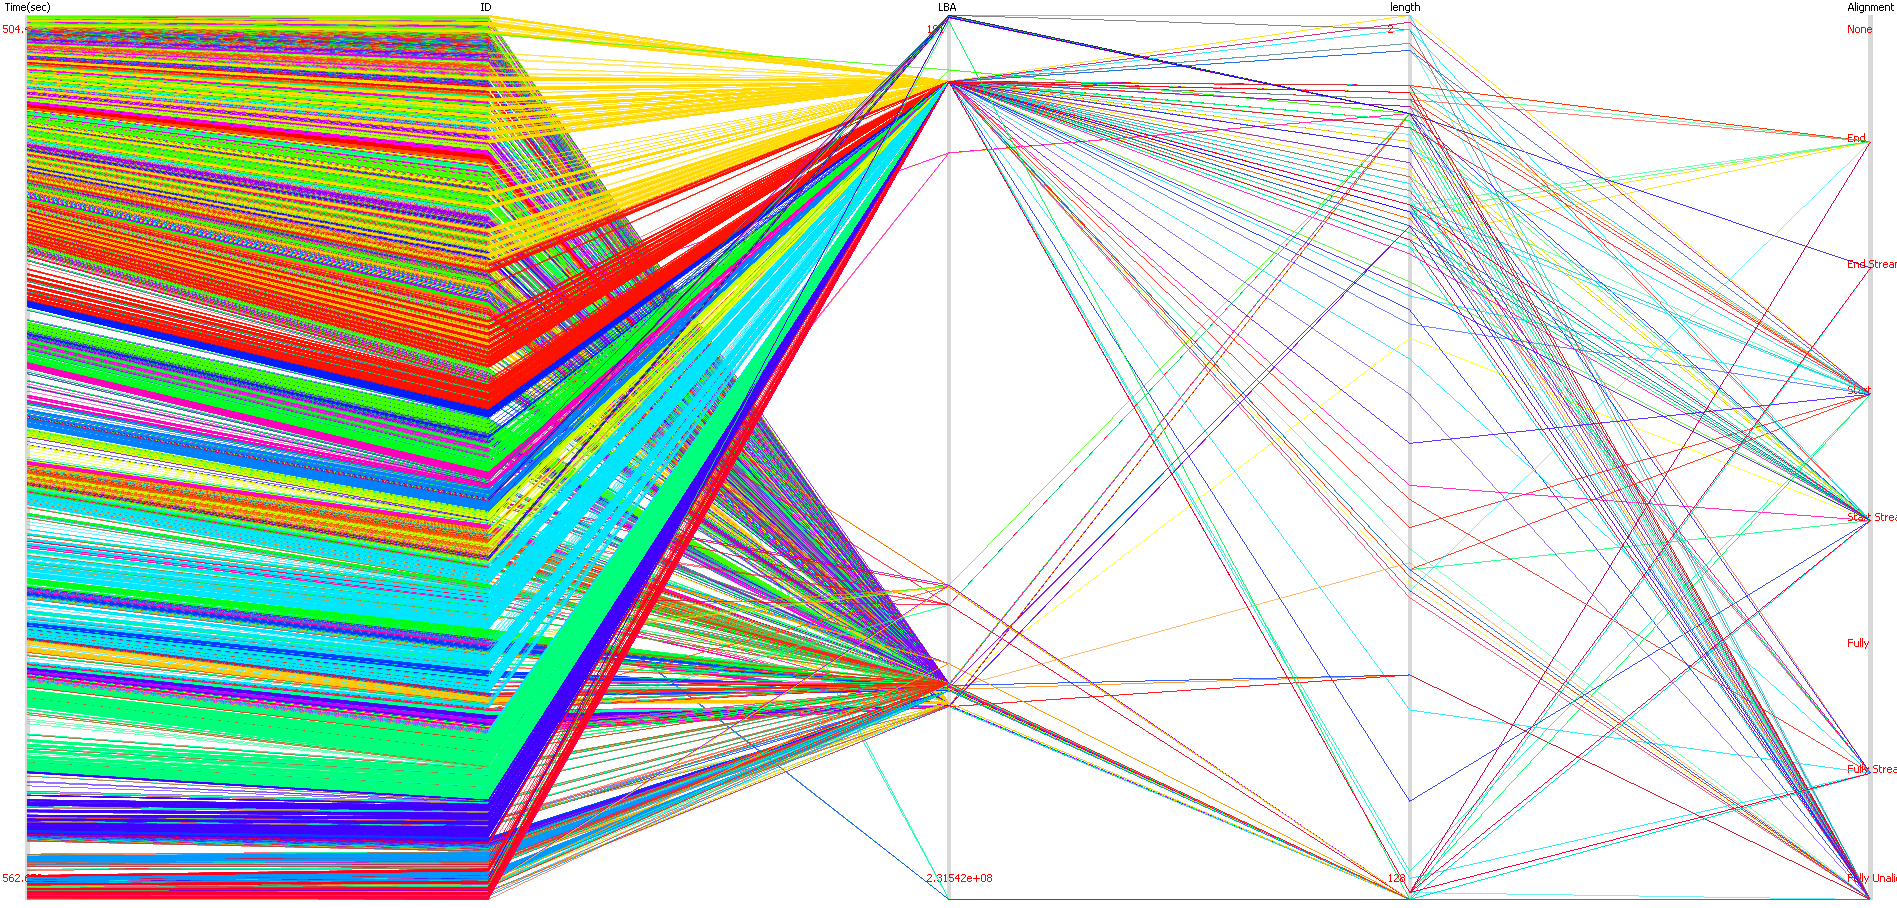
\includegraphics[width=\textwidth]{images/6.jpg}
 \caption[Focus applied on a production workload with threads colored.]{A production storage system workload captured dataset obtained from a partner corporation with identified threads coloring, axes hidden, and a subset focus applied.}
\end{figure}

\begin{figure}[h!]
 \centering
 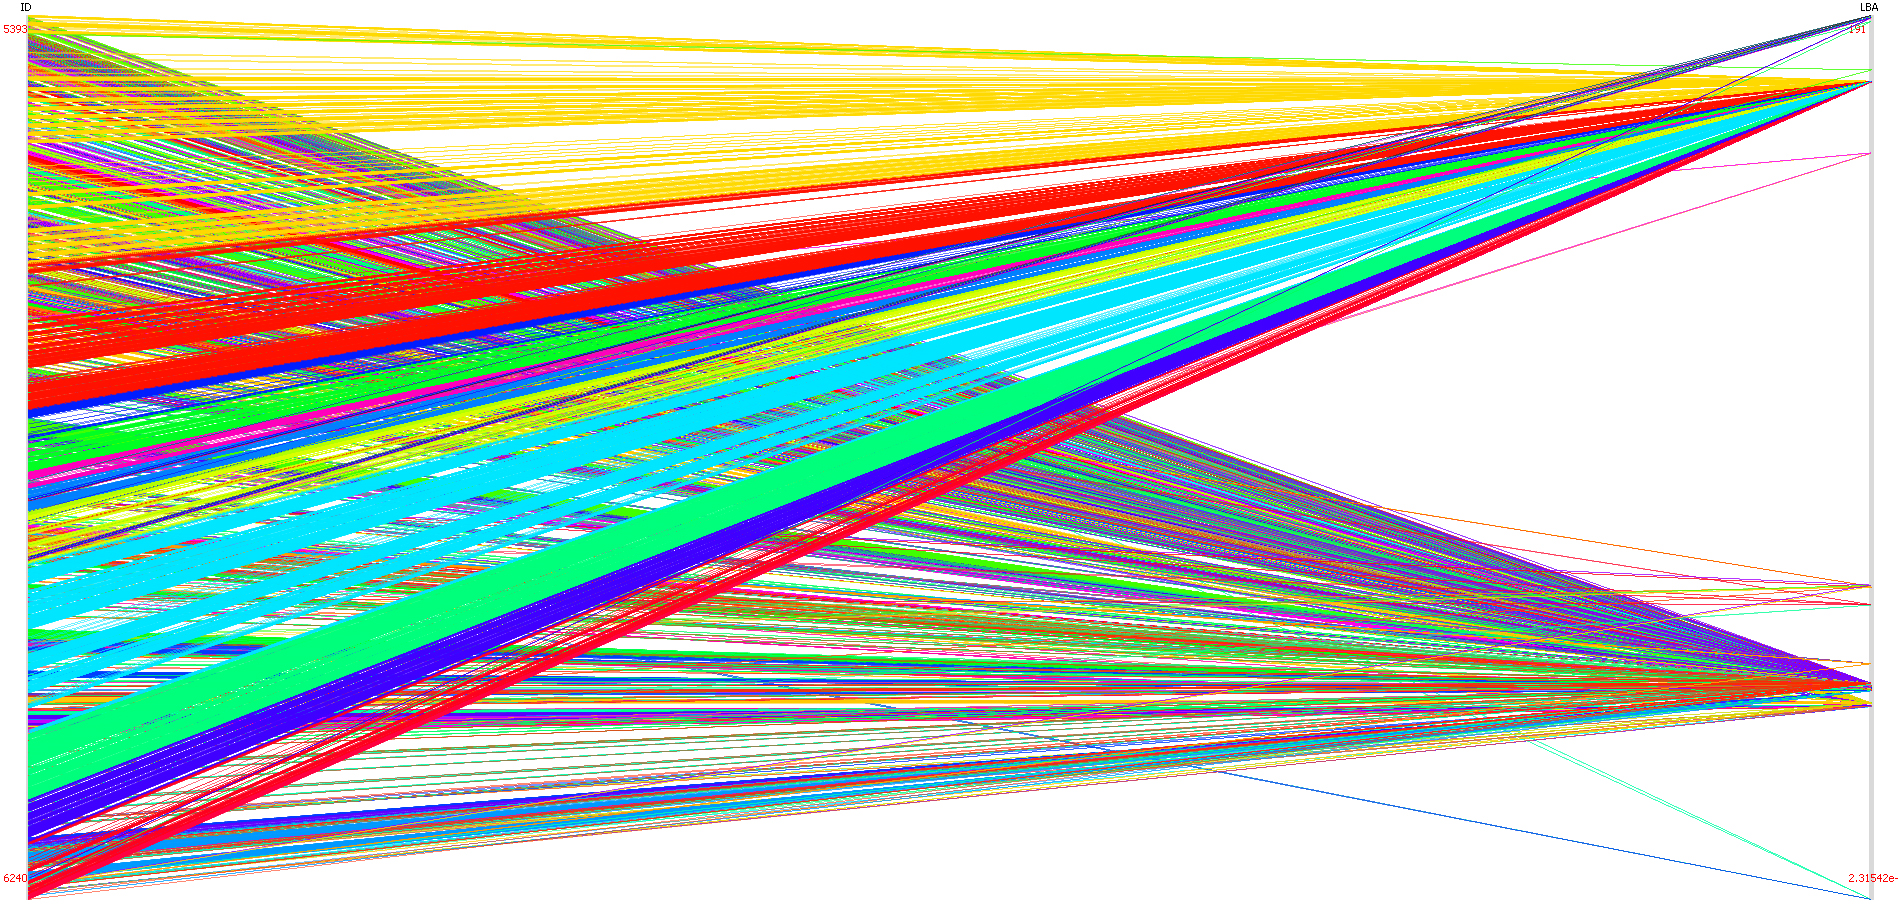
\includegraphics[width=\textwidth]{images/7.jpg}
 \caption[Focus applied on a production workload with threads colored.]{A production storage system workload captured dataset obtained from a partner corporation with identified threads coloring, axes hidden, and a subset focus applied.}
\end{figure}

\begin{figure}[h!]
 \centering
 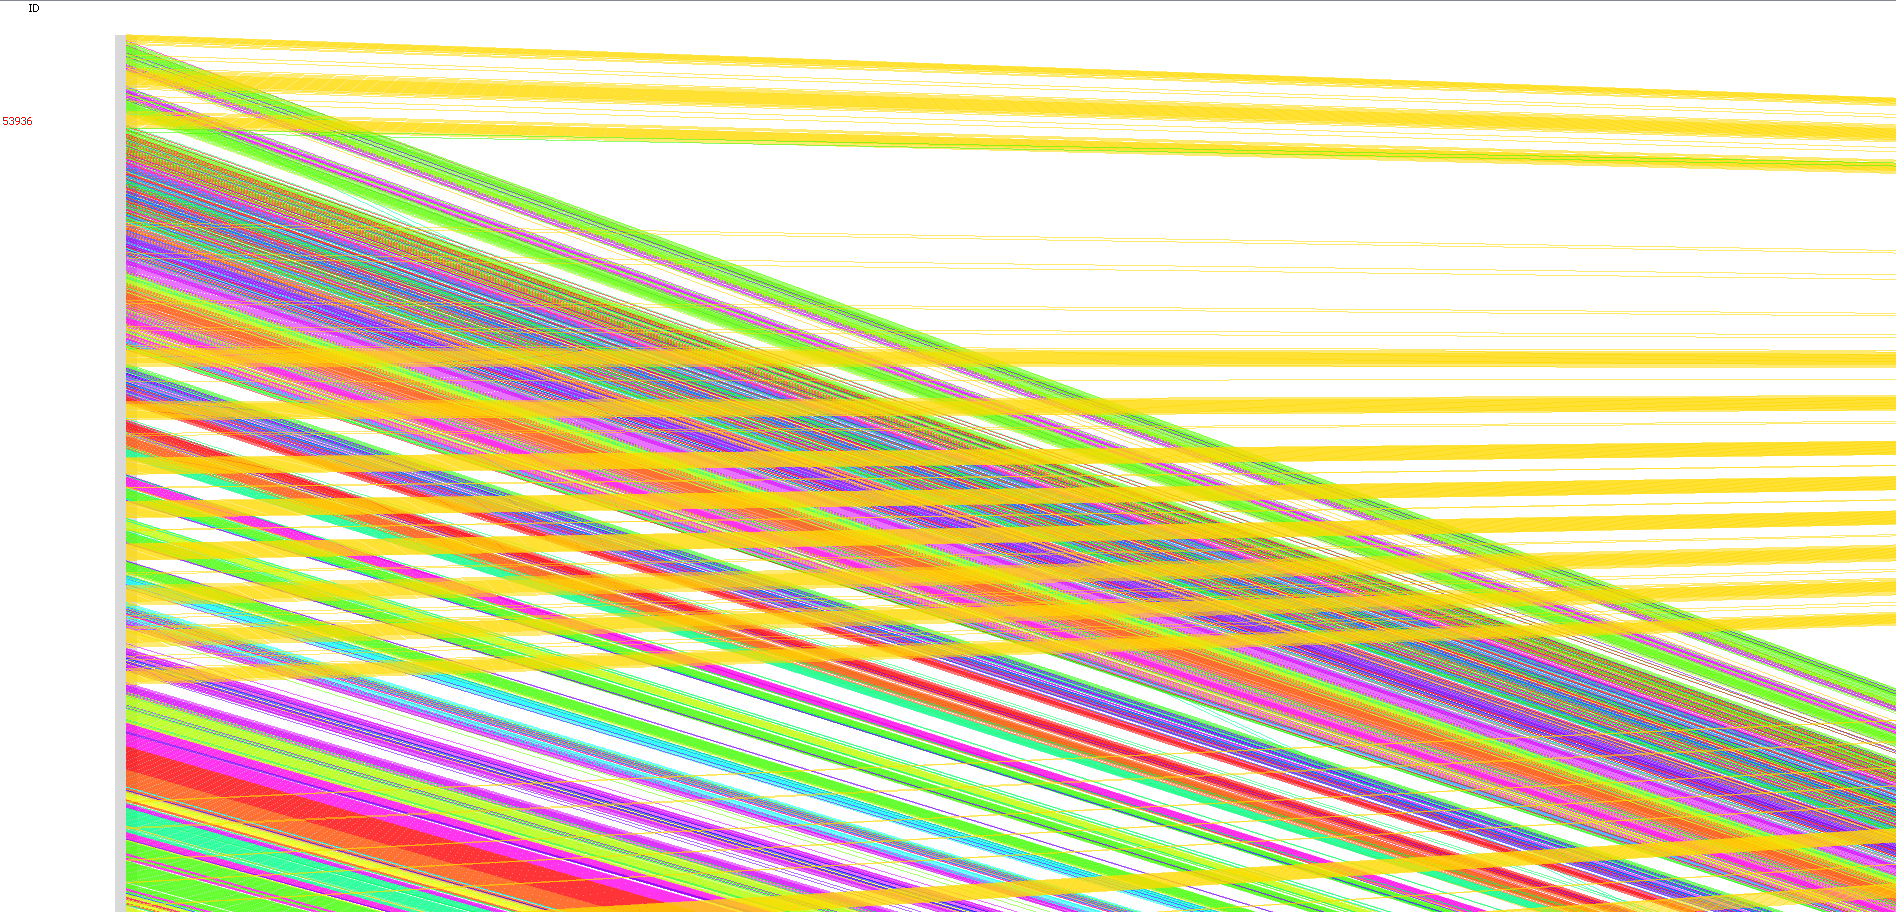
\includegraphics[width=\textwidth]{images/8.jpg}
 \caption[Focus applied on a production workload with threads colored.]{A production storage system workload captured dataset obtained from a partner corporation with identified threads coloring, axes rearrangement, a subset focus, and inward scaling applied.}
\end{figure}

\begin{figure}[h!]
 \centering
 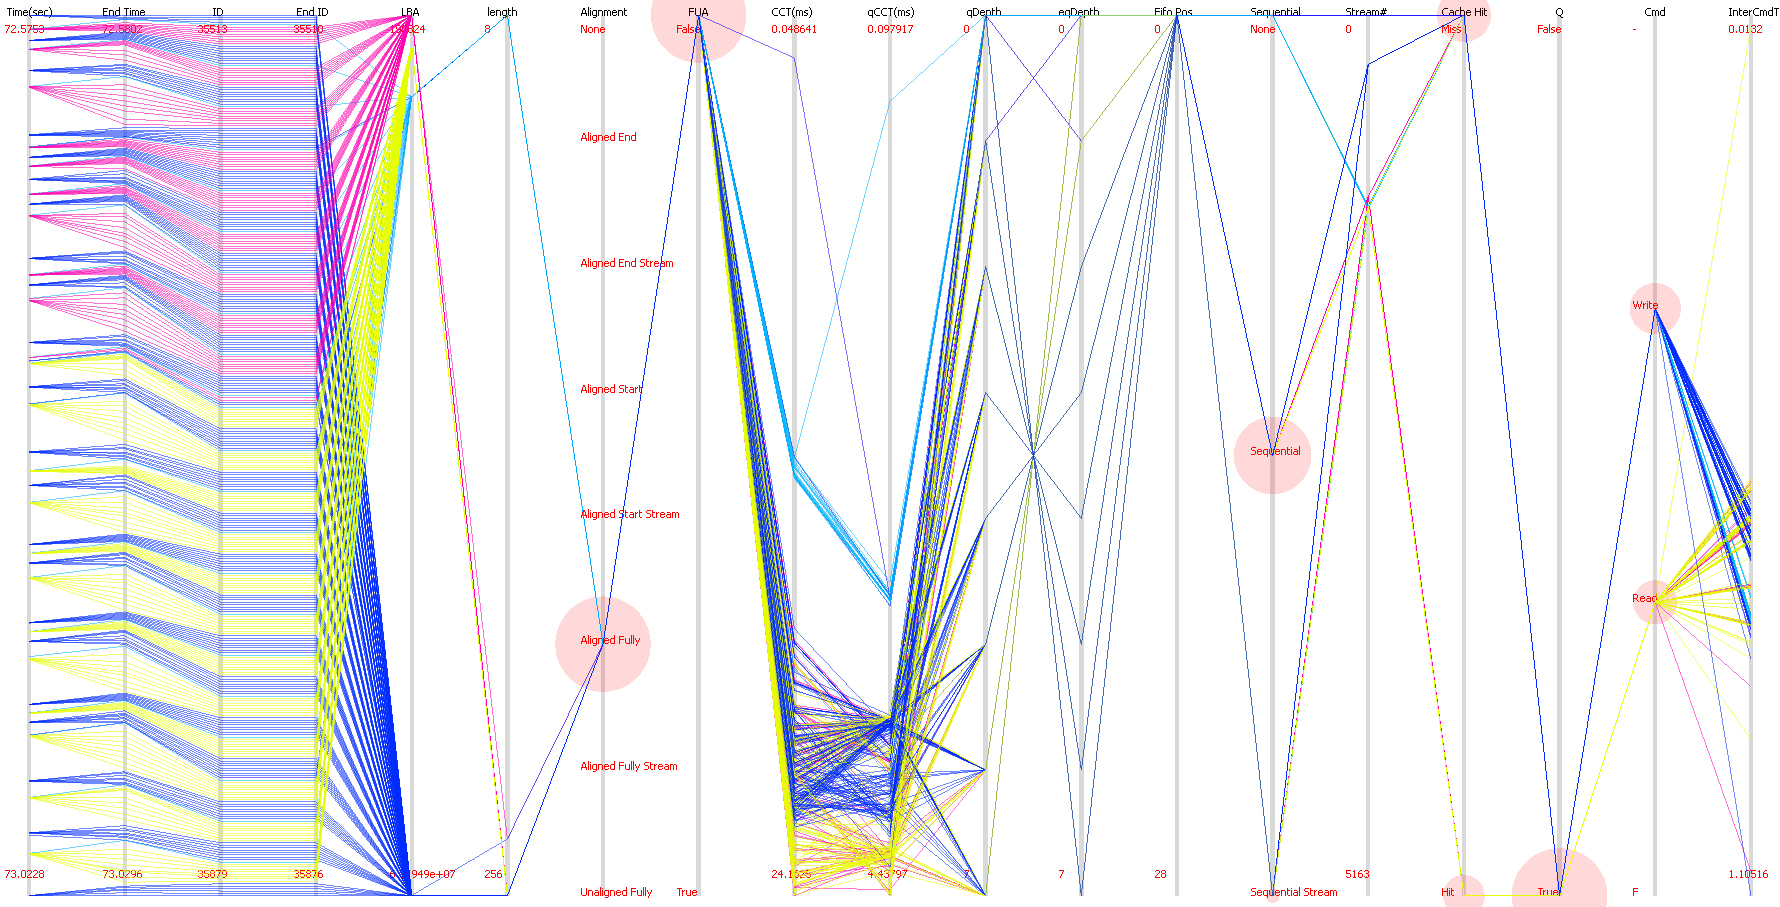
\includegraphics[width=\textwidth]{images/9.jpg}
 \caption[Focus applied on a test workload with threads colored.]{Overview of a test storage system workload dataset with identified threads coloring and a subset focus applied.}
\end{figure}

\begin{figure}[h!]
 \centering
 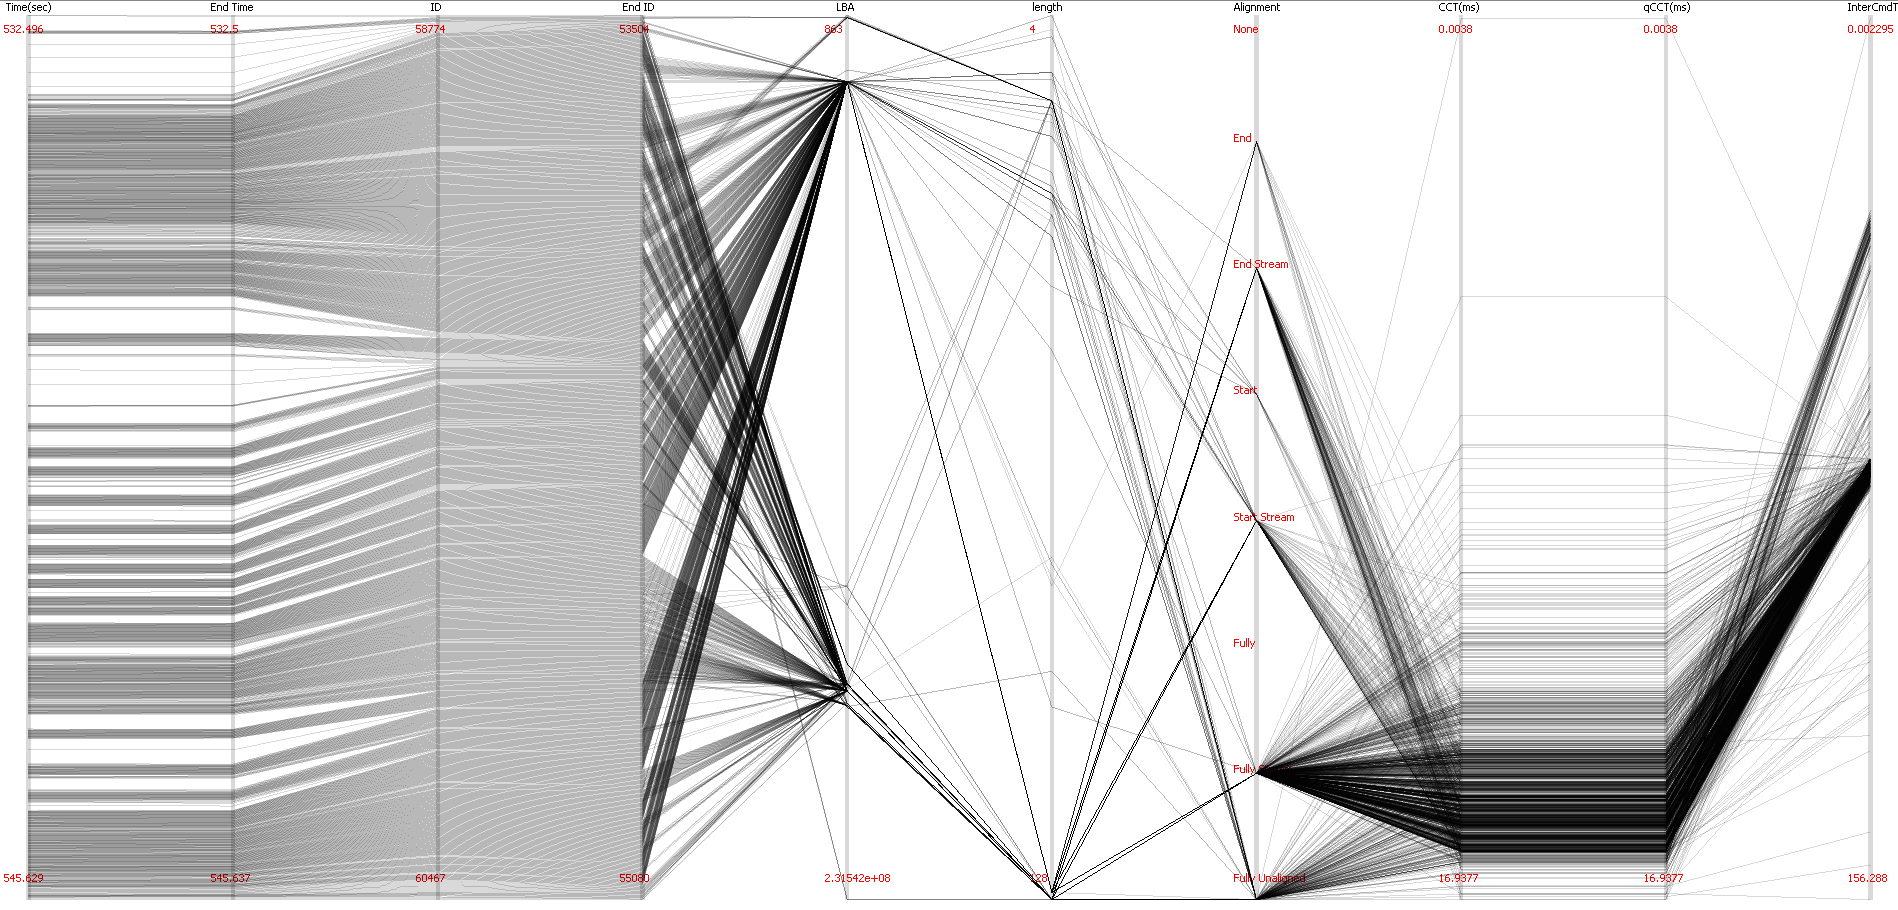
\includegraphics[width=\textwidth]{images/10.jpg}
 \caption[Focus applied on a production workload.]{A production storage system workload captured dataset obtained from a partner corporation with axes rearrangement and a subset focus applied.}
\end{figure}

\begin{figure}[h!]
 \centering
 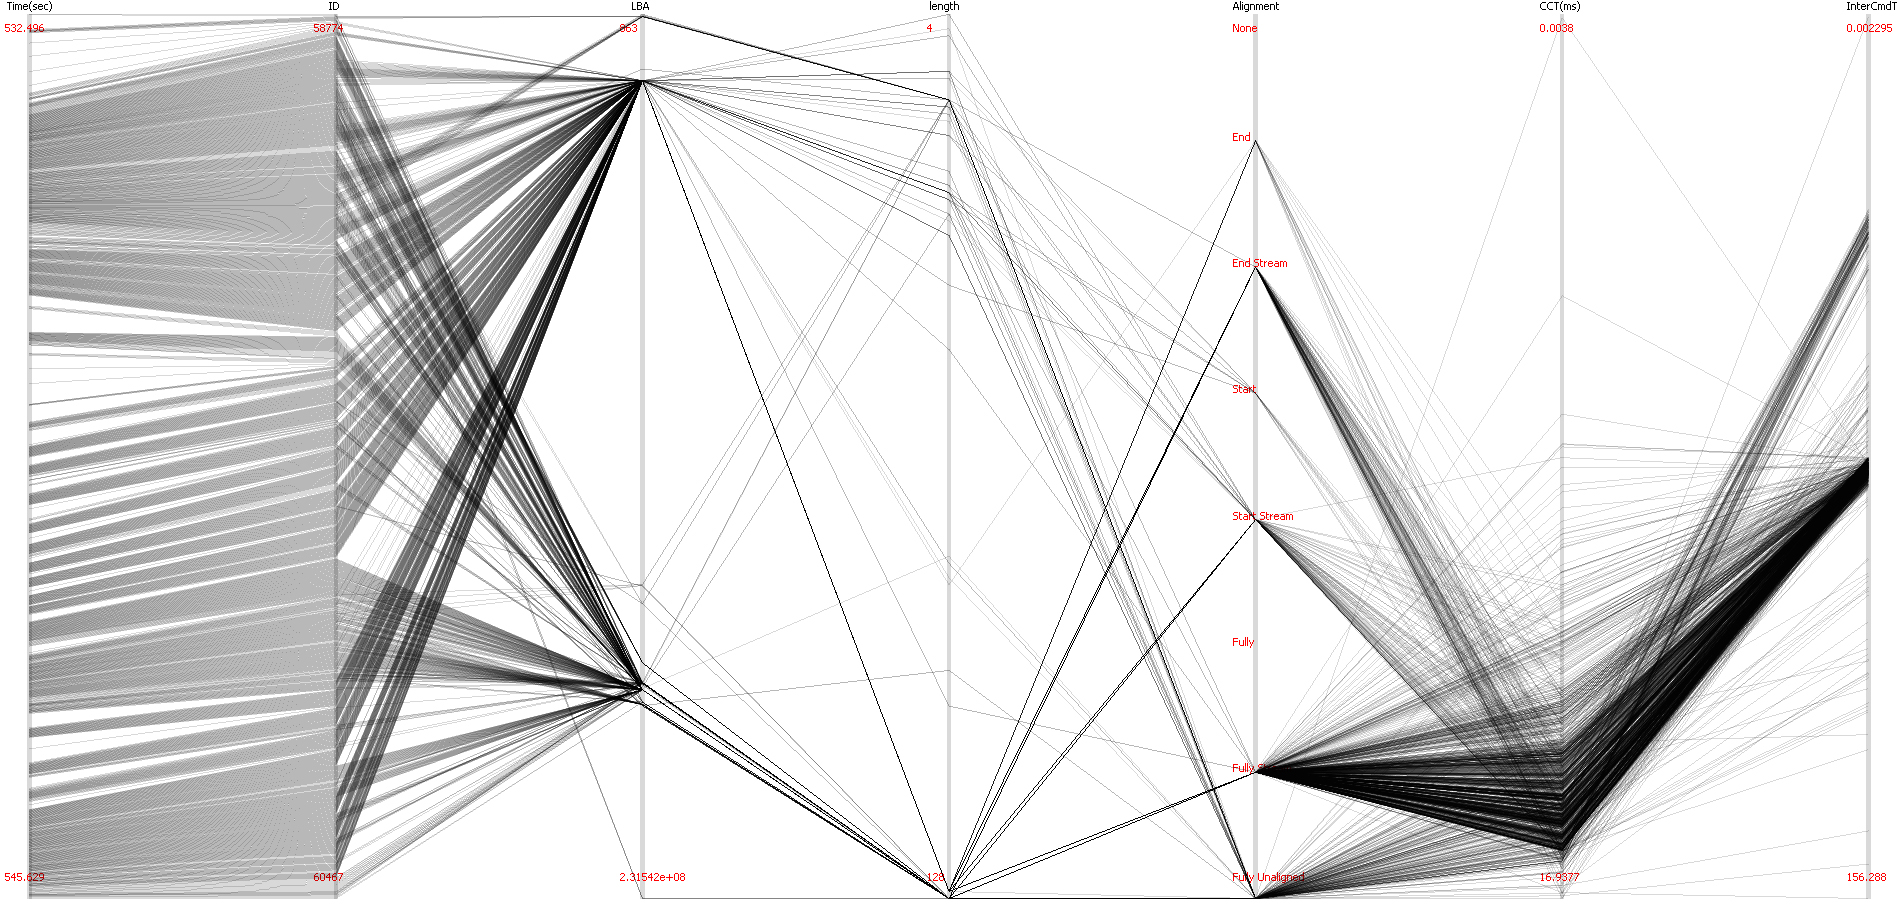
\includegraphics[width=\textwidth]{images/12.jpg}
 \caption[Focus applied on a production workload.]{A production storage system workload captured dataset obtained from a partner corporation with axes rearrangement and a subset focus applied.}
\end{figure}

\begin{figure}[h!]
 \centering
 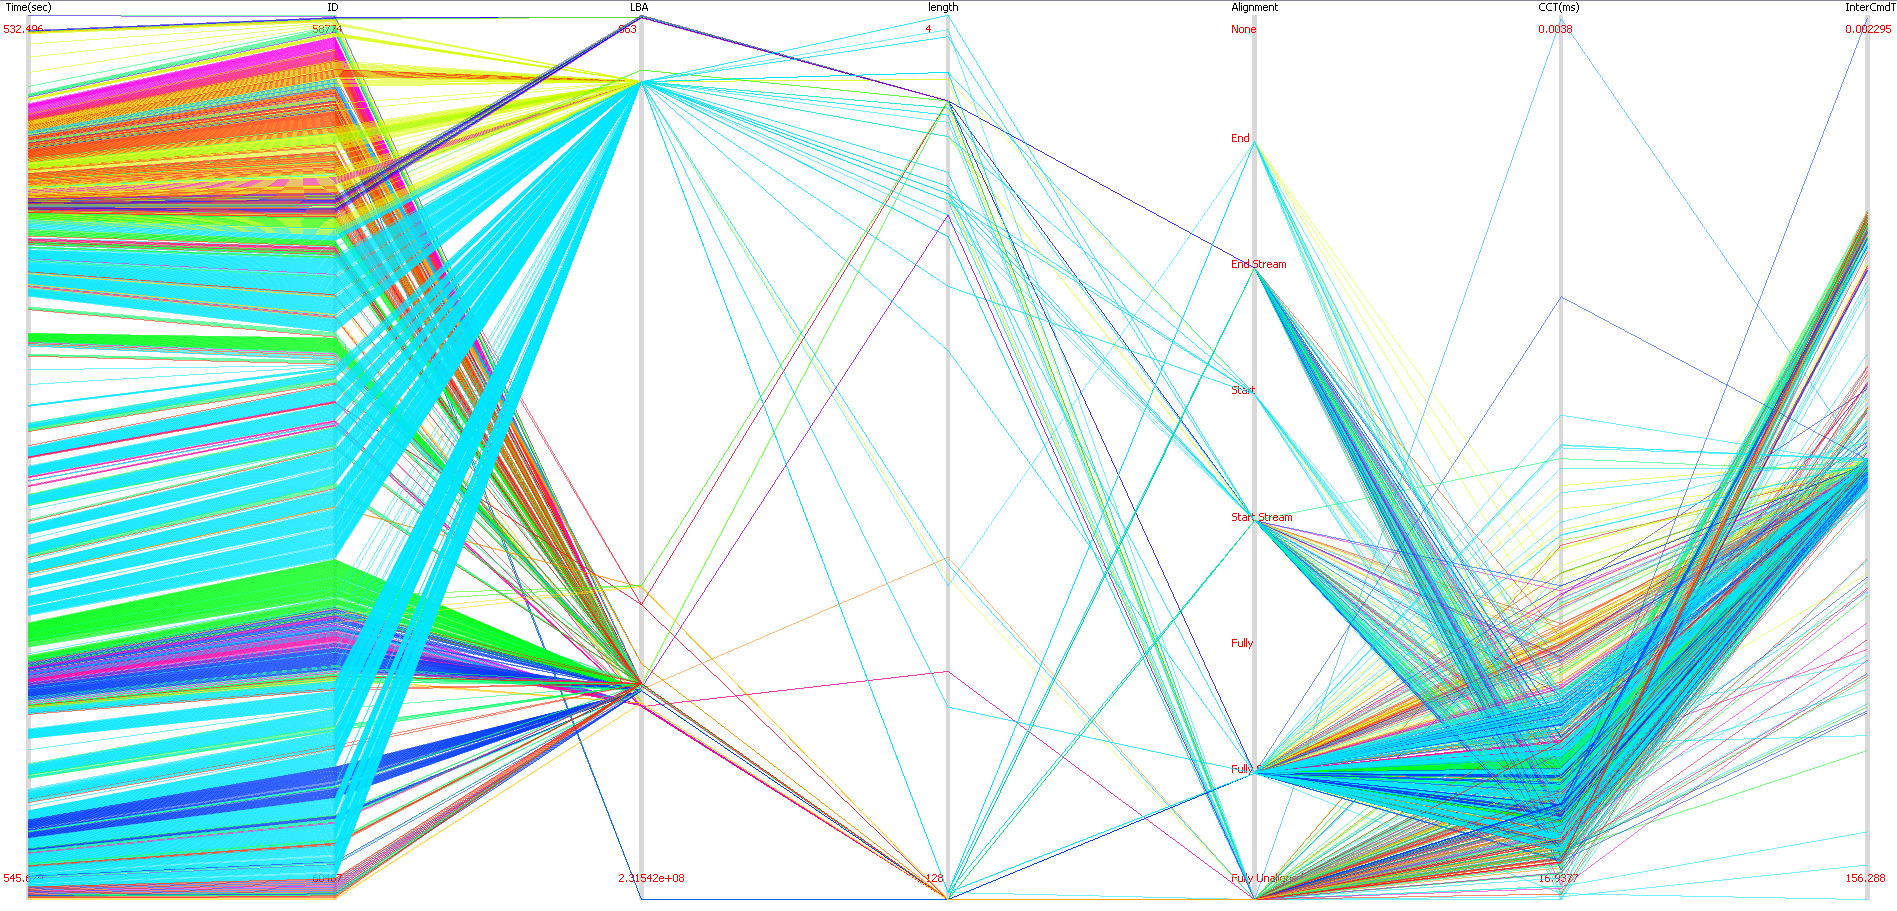
\includegraphics[width=\textwidth]{images/13.jpg}
 \caption[Focus applied on a production workload with threads colored.]{A production storage system workload captured dataset obtained from a partner corporation with identified threads coloring, axes rearrangement, and a subset focus applied.}
\end{figure}

\begin{figure}[h!]
 \centering
 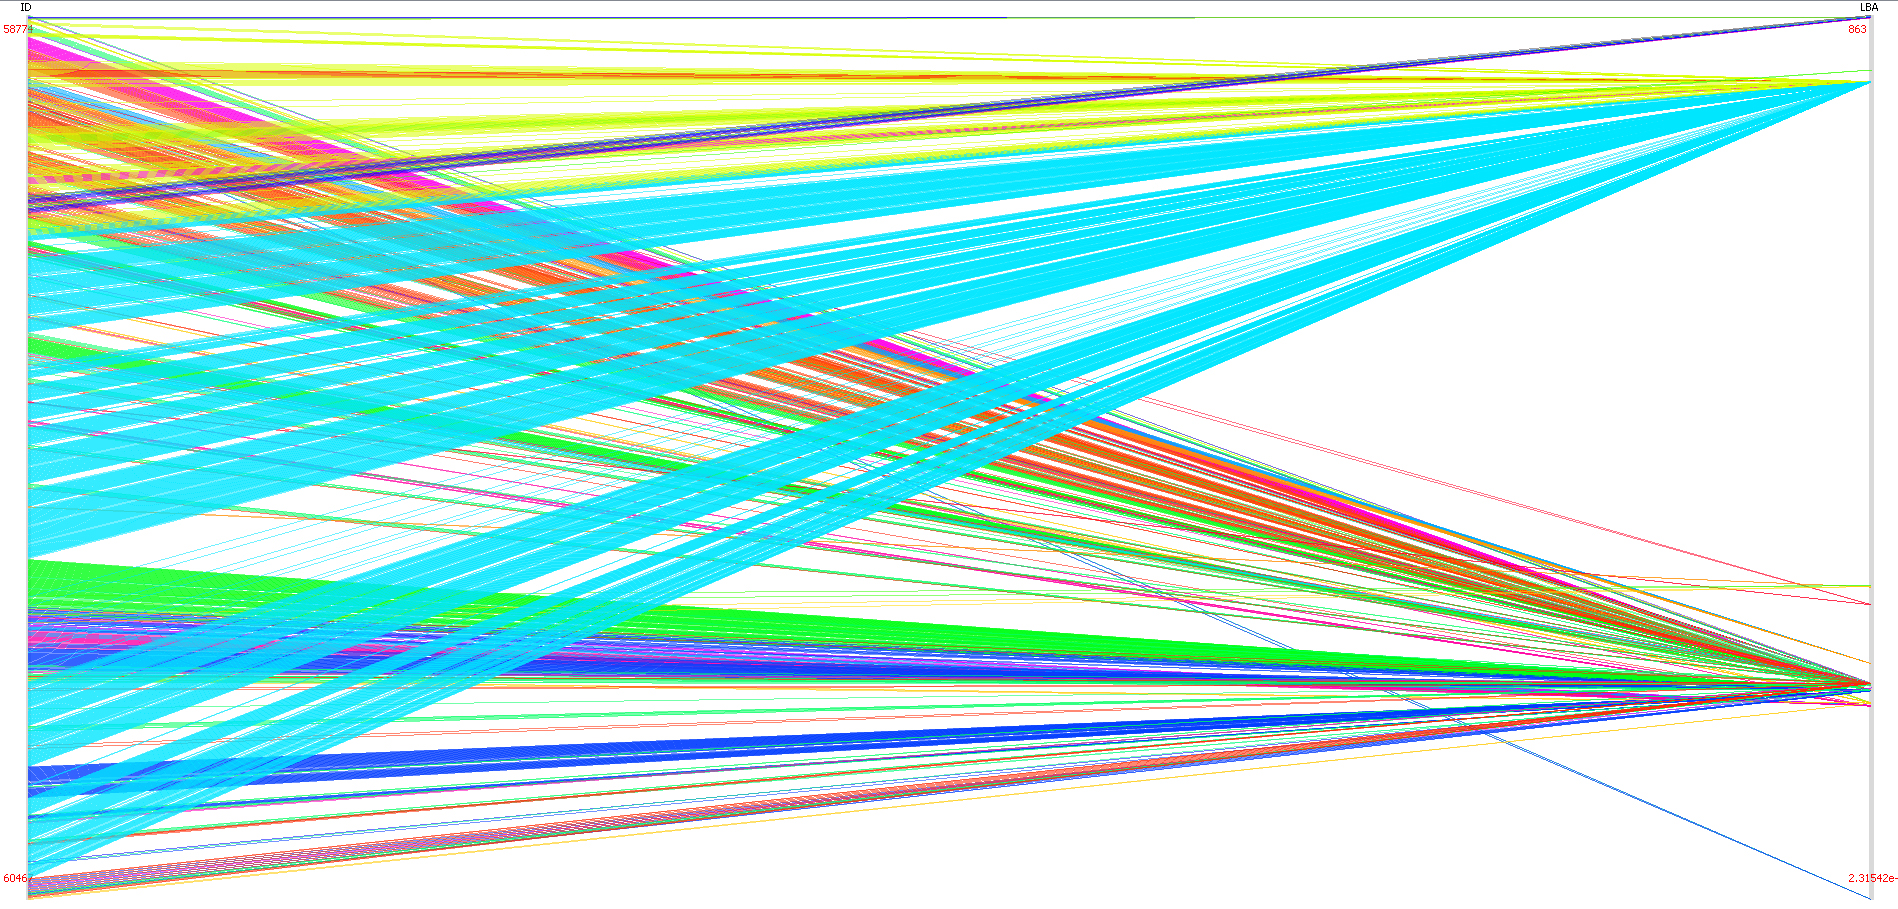
\includegraphics[width=\textwidth]{images/14.jpg}
 \caption[Focus applied on a production workload with threads colored.]{A production storage system workload captured dataset obtained from a partner corporation with identified threads coloring, axes hidden, and a subset focus applied.}
\end{figure}

\begin{figure}[h!]
 \centering
 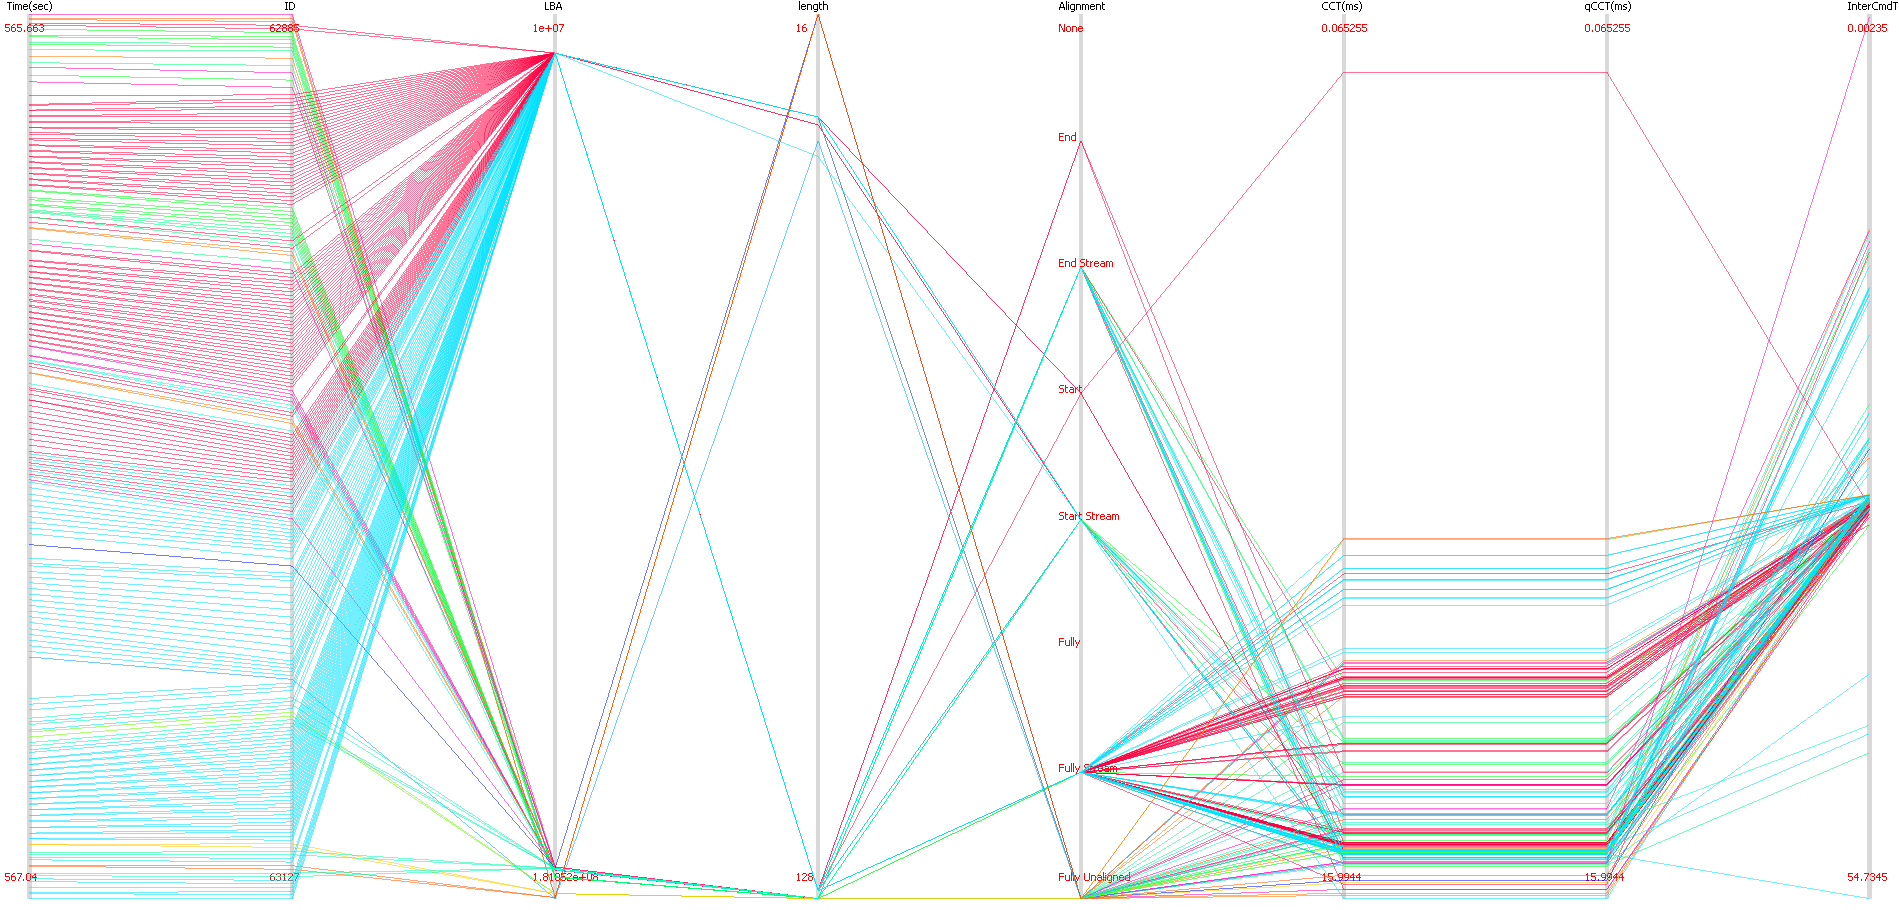
\includegraphics[width=\textwidth]{images/15.jpg}
 \caption[Focus applied on a production workload with threads colored.]{A production storage system workload captured dataset obtained from a partner corporation with identified threads coloring, axes hidden, and a subset focus applied.}
\end{figure}

\begin{figure}[h!]
 \centering
 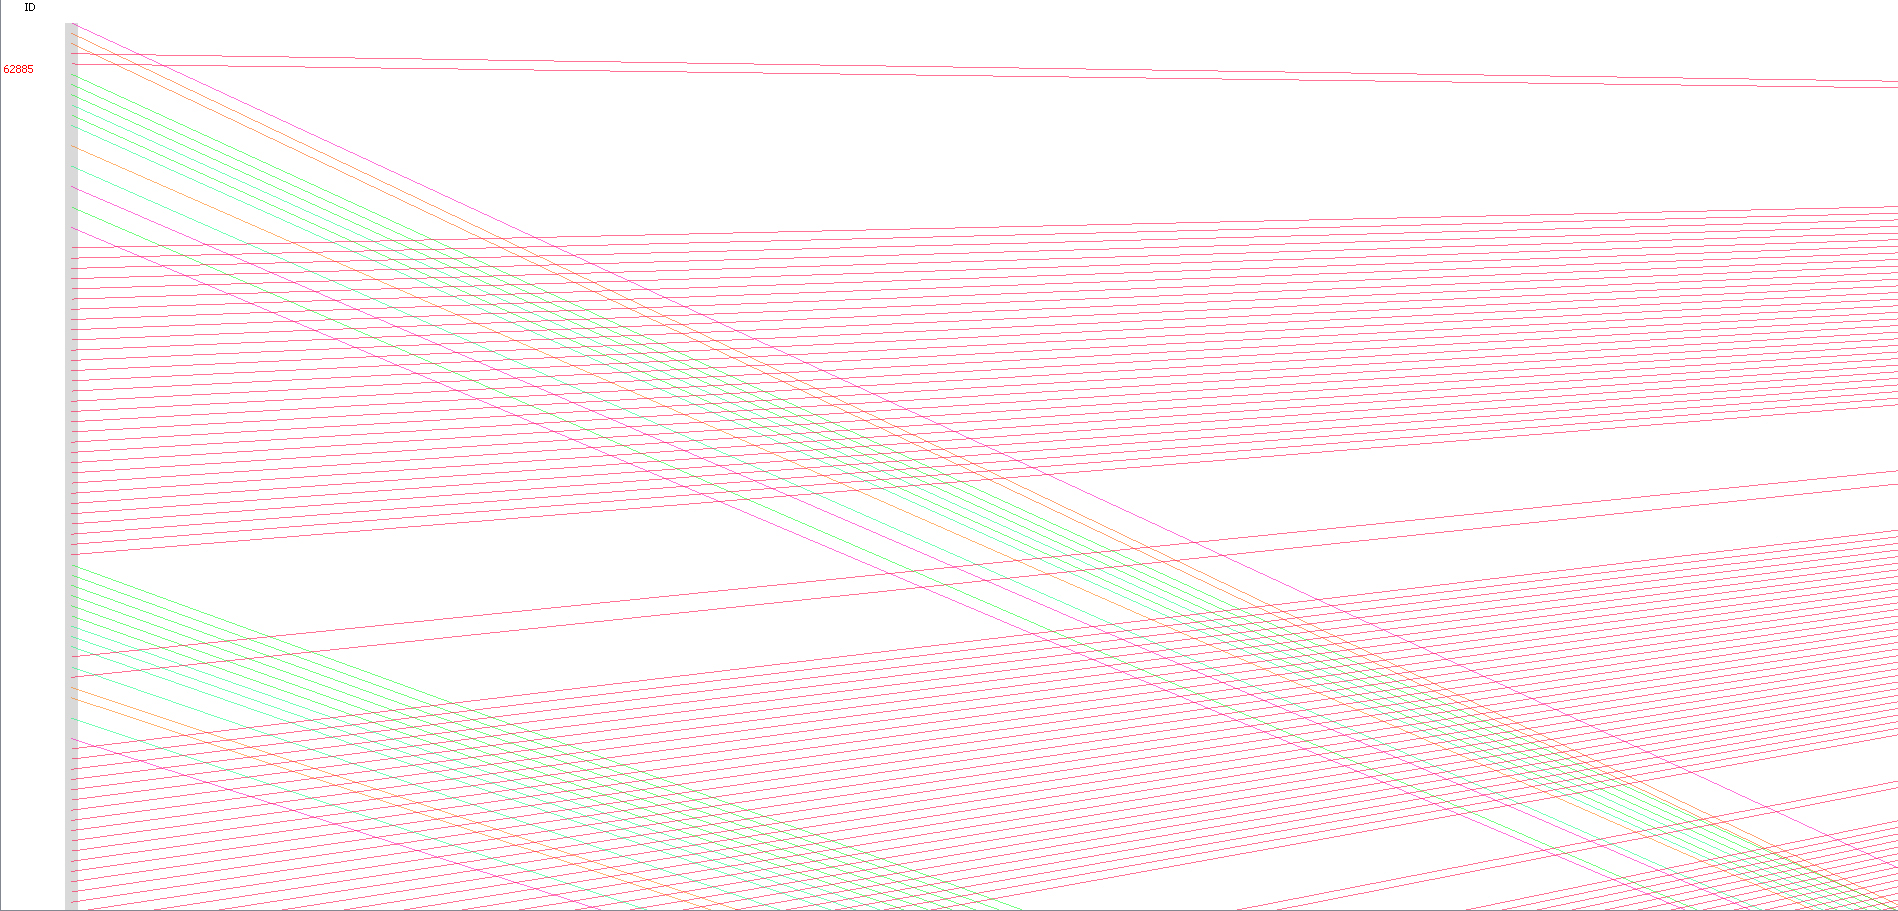
\includegraphics[width=\textwidth]{images/16.jpg}
 \caption[Focus applied on a production workload with threads colored.]{A production storage system workload captured dataset obtained from a partner corporation with identified threads coloring, axes rearrangement, a subset focus, and inward scaling applied.}
\end{figure}

\begin{figure}[h!]
 \centering
 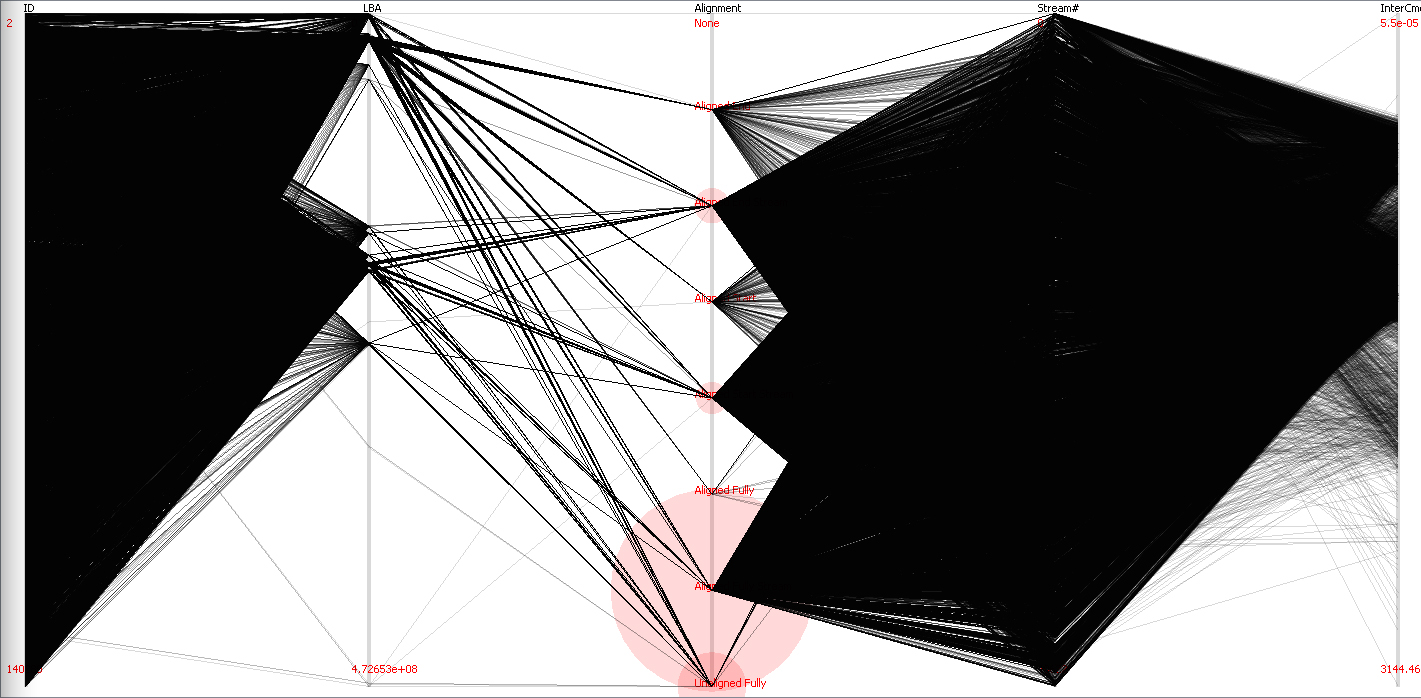
\includegraphics[width=\textwidth]{images/17.jpg}
 \caption[Production workload displaying Alignment distribution.]{A production storage system workload captured dataset obtained from a partner corporation with particular axes shown, displaying the distribution of Alignment values across the dataset.}
\end{figure}

\clearpage

\section{Tool Comparison}
In order to validate our tool, we obtained a production data center capture from a corporate internal mailing service, for the purposes of analyzing their workloads and identifying areas for improving disk utilization. We analyzed these datasets with both traditional analysis tools and our parallel coordinates tool with the assistance of domain experts at Western Digital and made similar discoveries. A comparison between our visualization and current tools used to analyze the same datasets are illustrated in the following figures. Figure \ref{fig:prev_tool} displays the output of a current tool utilized to identify the occurrence of LBA banding, the act of alternating between two LBA bands. LBA banding introduces seek overhead as the drive read-write head must travel back and forth between each LBA band, possibly leading to waiting for full disk revolutions prior to performing the requested operation. This occurrence can lead to a low queue environment, equating to low throughput, and consequently the potential for poor reliability as the drive is subject to adjacent-track interference (ATI), and an uneven spreading of disk lubrication~\cite{internal:collab}. 

\begin{figure}[h!]
 \centering
 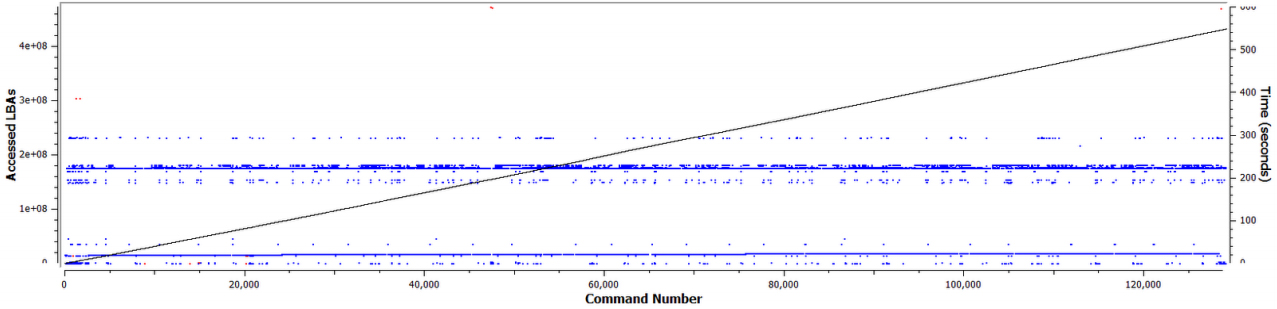
\includegraphics[width=\textwidth]{images/prev_tool.jpg}
 \caption[Output of a tool currently used to identify LBA banding.]{Output of a tool currently used by our collaborators to identify the occurrence of LBA banding, plotting Accessed LBAs on the left, Command Number on the bottom, and Time on the right~\cite{internal:collab}.}
 \label{fig:prev_tool}
\end{figure}

We display the same dataset in Figure \ref{fig:lba_banding_full}, which also exhibits the same density of accesses across the LBA axis when compared to the prior figure, captured with current tools. In both figures, there are a few accesses occurring at the highest LBA values, such as 4.72653\e{8}, while a majority of accesses across the capture occur at LBA bands in the lower half of LBA values in this particular dataset. Furthermore, we create a focus between commands 62885 and 63127 arbitrarily in Figure \ref{fig:lba_banding}, which further illustrates the occurrence of LBA banding at block addresses 1.0\e{7} and 1.8105\e{7}. This displays LBA banding more clearly with the use of colors to display the various threads involved, and the alternating between two LBA bands through the time sequential commands (not to be confused with LBA sequential) of the capture. 

\clearpage

\begin{figure}[htb!]
 \centering
 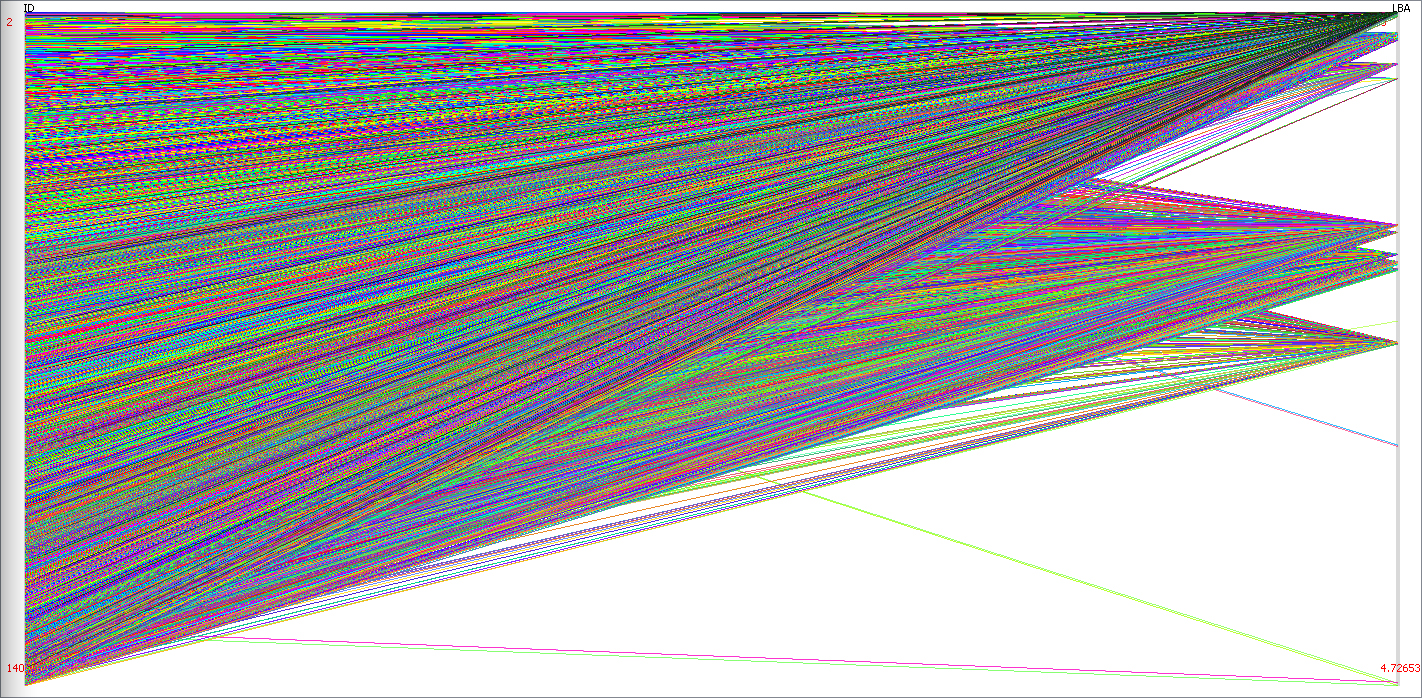
\includegraphics[width=\textwidth]{images/lba_banding_full.jpg}
 \caption[Output of our tool identifying the occurrence of LBA banding.]{Output of our tool identifying the occurrence of LBA banding, plotting Command ID on the left and LBA on the right~\cite{internal:collab}.}
 \label{fig:lba_banding_full}
\end{figure}

\begin{figure}[htb!]
 \centering
 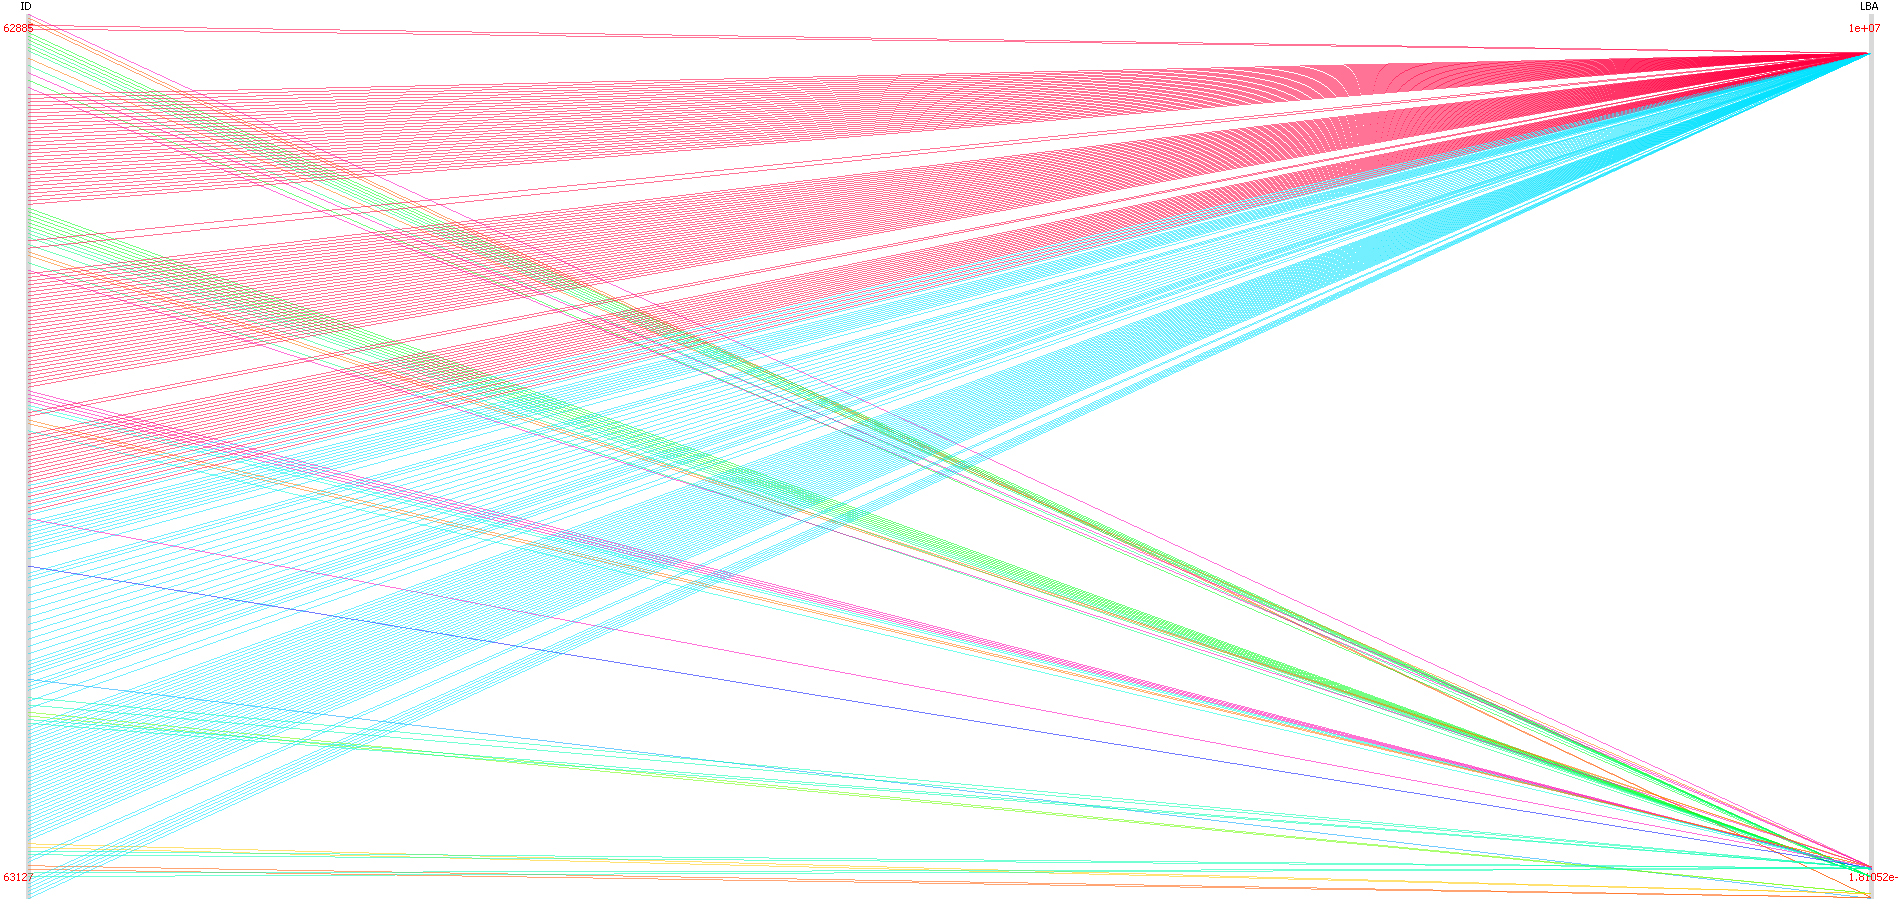
\includegraphics[width=\textwidth]{images/11.jpg}
 \caption[Output of our tool identifying the occurrence of LBA banding.]{Output of our tool identifying the occurrence of LBA banding, plotting Command ID on the left and LBA on the right~\cite{internal:collab}.}
 \label{fig:lba_banding}
\end{figure}

Lastly, we present Figure \ref{fig:no_queue} to illustrate the consequences of LBA banding by analyzing the following axes: Time, Command ID, LBA, Command Completion Time (CCT), Queue Command Completion Time (qCCT), Queue Depth (qDepth), End Queue Depth (eqDepth), FIFO Position, and Queueable. As we explained previously, LBA banding can lead to a low queue environment; in this dataset, the queue utilization was nonexistent as seen by observing the zero values of all records on the Queue Depth and End Queue Depth dimensions. There is no variation in the values between Command Completion Time and Queue Command Completion Time without queue utilization. Furthermore, every command in this dataset is identified as being queueable. The lack of utilizing command queueing to optimize the order in which access commands are executed indicates that unnecessary drive read-write head movement is likely occurring, which results in a decrease in performance, and consequently increased wear on storage media for workload environments consisting of multiple simultaneous read and write requests, an often occurrence in server-type applications~\cite{ncq:whitepaper}.

\begin{figure}[htb!]
 \centering
 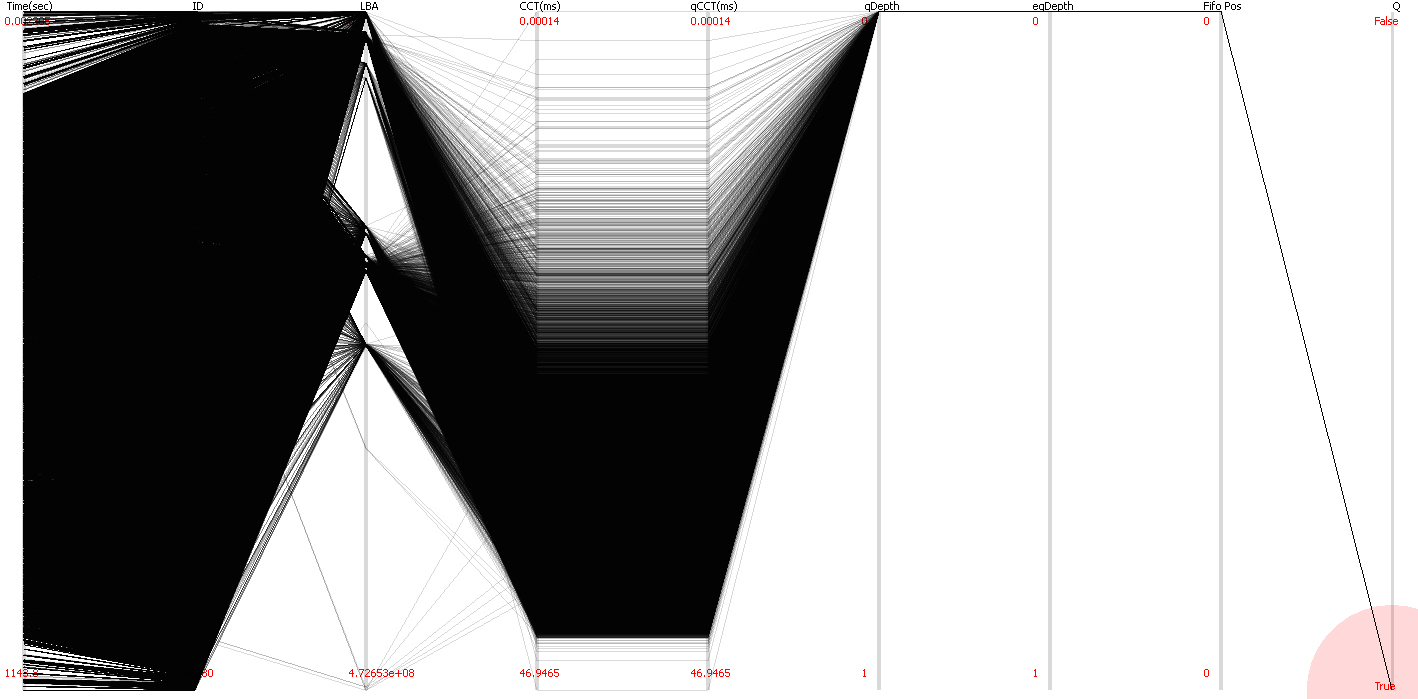
\includegraphics[width=\textwidth]{images/no_queue.jpg}
 \caption[Output of our tool identifying the occurrence of LBA banding.]{Output of our tool identifying the occurrence of LBA banding, showing a lack of queue utilization in an overview mode~\cite{internal:collab}.}
 \label{fig:no_queue}
\end{figure}

These results contribute to the validation of our tool as an effective approach for extracting valuable information from data center captures in order to identify inefficiencies in disk utilization of data storage systems. Furthermore, we introduce our tool to domain experts, academic professors, and graduate students to determine the usability of our visualization application.

\section{User Study}
We conducted a user study in order to determine the effectiveness of our visualization, as well as gather feedback regarding areas of future work. Our user study primarily focused on the ability to convey information from the workload datasets, illustrate general trends and outliers, and the usability of navigating the tool and manipulating the data. We designed our study to incorporate both quantifiable and open-ended channels of feedback in order to refrain from limiting users from expressing ideas for future work.

Our user group consists of domain experts at Western Digital, electrical engineering and computer science professors, and graduate students. Overall, the feedback was generally positive regarding both the effectiveness and usability of our tool. The limitations expressed in this study are identified as our known limitations. Quantifiable questions yielded a 3.5 average regarding the clarity of labeling in the tool, and a 5.0 average regarding the understanding of our thread coloring visualization, both on a 5.0 scale. Both the user study questions and responses can be found in Appendix \ref{app:user_study}, along with the documentation of our tool in Appendix \ref{tool:doc} provided to our users during the user study.

\section{Known Limitations}
We have been able to identify the following limitations in usability and overall effectiveness with the participants in our user study, especially domain experts. It would be more intuitive to perform axis rearranging with drag and drop actions, rather than through the current use of context menus to address usability. Similarly, for selecting the range of data to create a focus on, or brush and highlight, it would be useful to also have the option to click and drag to select ranges within a bounding box.

We gathered that the ability to set and compare multiple focus ranges simultaneously would be a valuable feature in order to increase the effectiveness of our tool. The choice of function and particular axes naming should be explored as well, taking into account recommendations of domain experts of whom this tool is intended for. A few other limitations were expressed, which classify as both usability and effectiveness, namely the ability to undo sequential user commands in the tool, and the ability to save and reload states of the visualization model while using the tool. Some of these limitations were understood prior to the user study and acknowledged as areas that can be addressed with advances in rendering performance, left as future work. 

\section{Conclusion}
This paper discusses the value for a comprehensive visualization tool aimed to specifically model data storage system captures. We attempted our initial approach to modeling such data, and while it was a novel method of visualization, we decided it was unable to effectively communicate the full dataset across all dimensions. Next, we found parallel coordinates as a widely used, effective approach for modeling multidimensional data, and described other related works that have implemented variations tailored towards particular domain applications. We then presented our implementation, which fully models data storage system trace captures and provides a range of features for user manipulation in order to focus on particular areas of interest. Through our user study, we found that our tool effectively conveys trends and outliers, and serves as a valuable tool for analyzing storage system datasets in comparison to current tools available. We also discovered through feedback that there are some limitations to our tool concerning usability as well as additional functionality.

In the industry of data storage system design and administration, this analysis tool provides insight into the design and deployment of small to large-scale storage systems. As the trend in mass data storage utilization continues to grow, it will be increasingly valuable to identify inefficiencies in storage system design and deployment regarding storage access algorithms, in order to minimize costly failures or underutilized storage media.

\chapter{Future Work}
\label{future_work}
This tool can be further developed to address limitations identified in our user study regarding usability and effectiveness through additional features. Some of the limitations identified are dependent on rendering performance; therefore future work entails refinement of the rendering algorithms used, including implementations that utilize parallel computing. Further development will include modularizing the initial preprocessing of the data where machine algorithms can be further developed, and the user-interacting visualization aspect of this project where usability and visualization techniques can be further explored.

Future development of this work includes research both in information visualization and data mining. Work in information visualization may entail implementing functionality of related works, including the research we listed in this paper. It may also include research in novel additions to parallel coordinates, which could further assist in the visualization of storage system data.

Data mining is also a promising area of future work. We envision a modular approach, where many datasets are stored in a repository. Once a capture is chosen to be analyzed, a preceding step can utilize various data mining techniques to identify anomalies and other information, before proceeding to display these findings in the visualization for users to manipulate.

The analysis of large datasets is a difficult task. Incorporating research in both data mining and information visualization as complementary approaches ensures that information can be gained from these datasets with both the statistical and exhaustive characteristics of machine learning, and the cognitive ability to intuitively analyze visual representations through human interaction.

% ------------- End main chapters ----------------------

\clearpage
\bibliography{bibliography}
\bibliographystyle{plain}
%\addcontentsline{toc}{chapter}{Bibliography}

\appendix 
\chapter{User Study} 
\label{app:user_study}
\section{User Study Questions}
\label{questions}
\textbf{Instructions:}
\begin{enumerate}
\item Make sure to give the documentation page a read
\item Download the thesispkg.zip file, unzip
\item Launch StorageSystemAnalyzer.exe
\item Click File---Open---Starting Application.csv for this study
\end{enumerate}

\textbf{Questions:}

\begin{enumerate}
\item How well do you understand the meaning of the text labels throughout the visualization? Please rate your understanding on a quantitative scale of 1-5, 1 being: ``I have no idea what these labels mean'' and 5 being: ``I completely understand the labels''.

\item Suggestions for labels (regarding question 1).

\item How well do you understand the purpose of the ``Color Threads" mode? Please go through the documentation and try coloring threads (it may be helpful to focus on a particular time/command\_id/LBA range) before answering this question. Rate your understanding on a quantitative scale of 1-5, 1 being: ``I have no idea what `Color Threads' does besides showing me crazy colors.'' and 5 being: ``I completely understand what `Color Threads' shows me".

\item Suggestions for coloring threads (regarding question 3).

\item What temporal trends do you notice of Read vs. Write commands in this data set? Please go through the documentation and try brushing ranges of data (hint: brushing certain ranges on a particular axis will be particularly helpful for noticing trends for this question).

\item Describe the interleaving occurring between command\_id's: 34550-37882. Please go through the documentation and perform the following steps before answering this question: 
\begin{itemize}
\item Focus on the command\_id axis between 34550 and 37882 
\item Enable the Color Threads mode 
\item Apply scaling (zoom in)
\item Hide other axes that are irrelevant.
\end{itemize}

\item Please provide any other general feedback, areas of improvement, and/or comments.

\end{enumerate}

\section{User Study Responses}
The following are responses to the user study questions in Section \ref{questions}.

\textbf{Dave Hamilton (Domain Expert at Western Digital):}
\begin{enumerate}
\item 3
\item The focus and brush concept were a little unusual compared to other visualization tools that I have used.
\item 5
\item The color thread mode needs to have settings for ``near" sequential in both time and LBA distance.
\item What I see is the workload starts with a large number of writes, then switches to interleaved read and writes.
\item There are several read and write streams that are almost evenly interleaved.
\item
\begin{itemize}
\item It would be nice to highlight a range on an axis for setting the focus range.
\item Drawing brush ranges should be done last so that the brush range is not over written by other data.
\item I couldn't set a focus on the Q Depth axis.
\item It would be nice to set several focus ranges simultaneously.
\end{itemize}
\end{enumerate}

\textbf{John Oliver (Electrical Engineering Professor at Cal Poly):}
\begin{enumerate}
\item 4
\item 
\begin{itemize}
\item Set Equation should be renamed ``Axes Scale"?
\item Create focus should be renamed ``Restrict Input"?
\item The ranges of labels get overwritten by the plot data.  The labels of the extremes should be placed outside the axis?
\end{itemize}
\item 5
\item 
\begin{itemize}
\item It may be nice to have multiple, different focus ranges
\item Not sure if you can support different focuses on different axes, however.
\end{itemize}
\item Reads-only first, writes-only last, interleaved in between.
\item Looks to me that the data is from two different ranges of LBAs.
\item Also, It would be nice to have the following features.
\begin{itemize}
\item Control-z should undo the last transformation.
\item It would be nice to be able to save a particular configuration of the tool.
\item What does the value of 1 or 0 mean for a cache hit?  Or 0-3 for Command?
\end{itemize}
\end{enumerate}

\textbf{Adam Miller (Computer Science Masters Student at Cal Poly):}
\begin{enumerate}
\item 5
\item (no comments)
\item 5
\item (no comments)
\item Initially read-heavy, followed by alternating reads/writes, and finally a long stream of writes.
\item Interleaving between at least 6 threads. One thread is present through the whole range while the other 5 vary in how long they are alive.
\item In general I like the tool. I'm not sure a good alternative, but right-clicking for the context menu to create focuses, set brushing, etc. feels overused. It might be good to have buttons where the button is pressed and then you select which field to apply to.
\end{enumerate}

\textbf{Chris Lupo (Computer Science Professor at Cal Poly):}
\begin{enumerate}
\item 3
\item I see no axis labels when running this, but I'm in Wine, so not a true indication of what your application is really doing.
\item 5
\item Really more related to Focus, but it'd be great to get changes in view with fewer steps (mouse clicks). Undo functionality would also be desirable.
\item It's not clear to me what the mapping is in the Command axis. I brush for a value of ``1", is that a read or a write, or otherwise? Perhaps the brush dialog should show textual values instead of numerical values for those axes where it's appropriate.

For the brushing of command ``1", I see a lot of commands early, then some interleaved commands, then none.
\item Interleaving of magenta and blue early on, yellow and blue in the middle and magenta and blue at the end of the range. There is some minor interleaving of light-blue throughout. I interpret this as four distinct threads in this command range.
\item My experience of using this tool in an interpreted environment shouldn't be used to guide your design decisions, with the exception of the ``coloring threads" comments above. However, this is an indication that the tool is not quite cross-platform ready yet, which likely is ok, just to be aware of.
\end{enumerate}

\chapter{Data Storage System Visualization Documentation}
\label{tool:doc}
The tool documentation presented to the participants of our user study to describe each of the features available to interact with the visualization, and how to apply them~\cite{steven:doc}.

\section{Axes}
Each axis represents a different dimension of data. You can trace each record through each of the dimensions to see, for instance, if a particular access is a read or a write, where it happened spatially (logical block address), when it happened (time/end time), whether it was a cache hit/miss, etc.

\subsection{Hide}
Axes can be concealed by right clicking on them, and selecting ``Remove Dimension".
\begin{figure}[htb!]
 \centering
 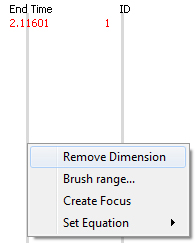
\includegraphics[width=0.5\textwidth]{images/documentation/remove_dimension.jpg}
 \caption[Right-clicking an axis to remove a dimension.]{Right-clicking an axis to invoke the context menu to remove a dimension.}
 \label{fig:doc}
\end{figure}

\subsection{Show}
Axes can be displayed again by right-clicking between two shown axes, selecting ``Insert", and choosing from a list of axes that are currently hidden.
\begin{figure}[htb!]
 \centering
 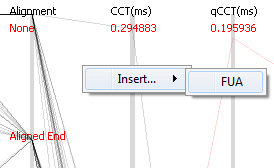
\includegraphics[width=0.5\textwidth]{images/documentation/insert_dimension.jpg}
 \caption[Right-clicking between two axes to insert a hidden dimension.]{Right-clicking between two axes to invoke the context menu to insert a hidden dimension.}
 \label{fig:doc}
\end{figure}

\clearpage

\subsection{Rearrange}
Currently, the method to rearrange axes are to use the methods above to hide an axis and insert it where desired. Future work will include a more intuitive method, such as dragging and dropping axes.

\subsection{Brush}
Brushing is a method used to highlight a particular range of data. Right-click on an axis and select ``Brush range..." which will launch a dialog to select a particular range to brush. Either use the sliders or manually enter the values for the range to highlight, click ``OK", and the range will now be highlighted in red. In ``Color Threads" mode, brushing is not shown.

\begin{figure}[htb!]
 \centering
 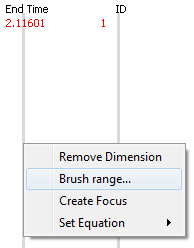
\includegraphics[width=0.5\textwidth]{images/documentation/brush_range.jpg}
 \caption[Right-clicking an axis to invoke the context menu to brush range.]{Right-clicking an axis to invoke the context menu to select a brush range.}
 \label{fig:doc}
\end{figure}

\begin{figure}[htb!]
 \centering
 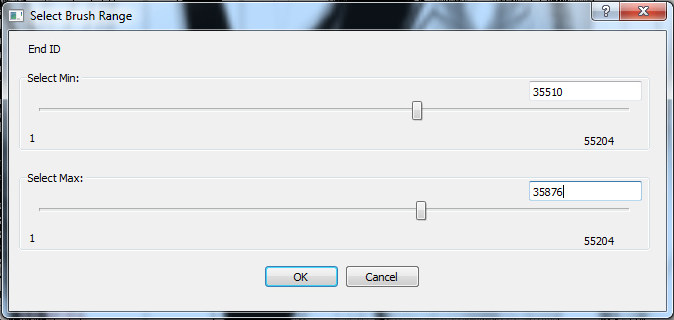
\includegraphics[width=\textwidth]{images/documentation/select_brush_range.jpg}
 \caption[The dialog presented to the user to select a range to brush.]{The dialog presented to the user to select a range to brush.}
 \label{fig:doc}
\end{figure}

\begin{figure}[htb!]
 \centering
 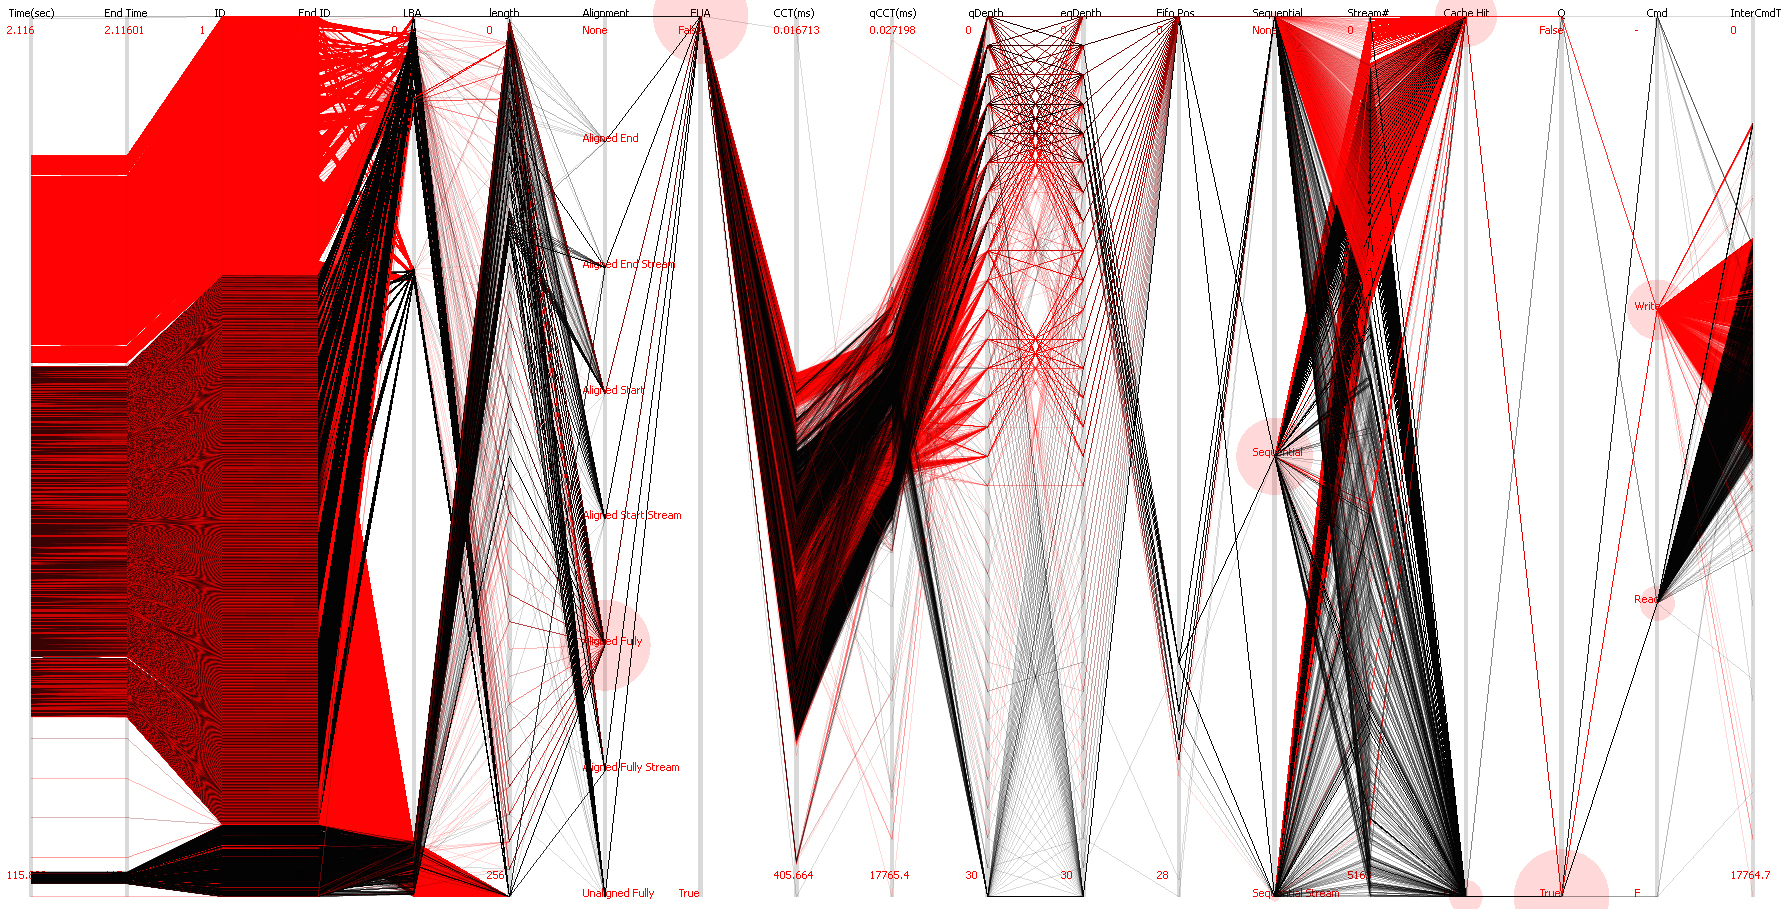
\includegraphics[width=\textwidth]{images/documentation/brush_overview.jpg}
 \caption[Overview of a brush applied to all Write commands.]{Overview of a brush applied to all Write commands.}
 \label{fig:doc}
\end{figure}

\subsection{Equation}
Certain dimensions contain data that is more appropriately displayed on a logarithmic or linear scale. To toggle a dimension's scale, right-click on the axis and choose the option under ``Set Equation" (the opposite of the currently set scale will appear in the menu, e.g. if a dimension is currently in linear scale mode, ``Logarithmic" will be displayed under ``Set Equation" when right-clicking on the axis.

\begin{figure}[htb!]
 \centering
 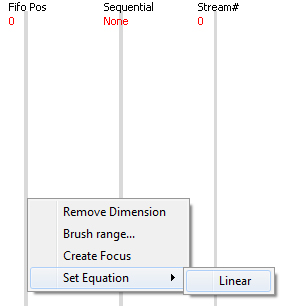
\includegraphics[width=0.5\textwidth]{images/documentation/set_linear.jpg}
 \caption[Right-clicking an axis to set the dimension scaling to linear.]{Right-clicking an axis to invoke the context menu to set the dimension scaling to linear.}
 \label{fig:doc}
\end{figure}

\begin{figure}[htb!]
 \centering
 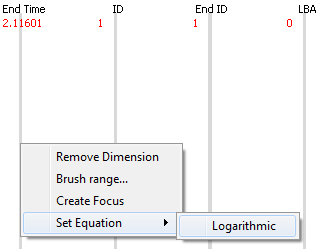
\includegraphics[width=0.5\textwidth]{images/documentation/set_logarithmic.jpg}
 \caption[Right-clicking an axis to set the dimension scaling to logarithmic.]{Right-clicking an axis to invoke the context menu to set the dimension scaling to logarithmic.}
 \label{fig:doc}
\end{figure}

\section{Modes}
There are three main modes to view data: Overview (default), Focus, and Color Threads.

\subsection{Overview Mode}
Overview is the default mode for viewing data, it displays every record and axis. Toggling between Overview and Focus is accomplished by clicking on the Mode menu at the top of the window, and selecting ``Overview" or ``Focus". These options will be greyed out when either: that mode is already displayed, or focus has not yet been initialized (this is done by the method below). Note: This is mutually exclusive to Focus mode.

\begin{figure}[htb!]
 \centering
 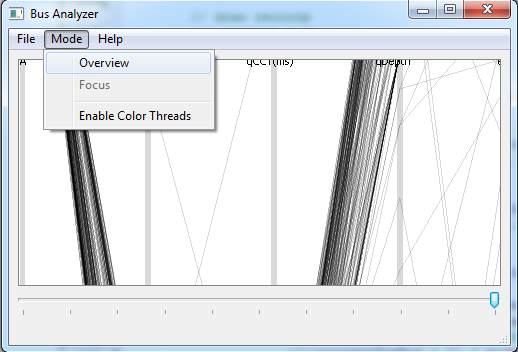
\includegraphics[width=\textwidth]{images/documentation/enable_overview.jpg}
 \caption[Enabling Overview mode through the use of the Mode menu.]{Enabling Overview mode through the use of the Mode menu.}
 \label{fig:doc}
\end{figure}

\begin{figure}[htb!]
 \centering
 \includegraphics[width=\textwidth]{images/documentation/overview.jpg}
 \caption[Overview mode displays all records of the dataset.]{Overview mode displays all records and axes of the dataset.}
 \label{fig:doc}
\end{figure}

\subsection{Focus Mode}
Focus is a mode which focuses on a particular range selected on a dimension. Similar to brushing, right-click on an axis and select ``Create Focus" which will launch a dialog to select a particular range to focus on. Either use the sliders or manually enter the values for the range to focus, click ``OK", and the visualization will now be adjusted to only display records that fall into that range. This focus extends to other dimensions as well, and modifies the circular histograms on discrete axes as well.

Toggling between Overview and Focus is accomplished by clicking on the Mode menu at the top of the window, and selecting ``Overview" or ``Focus". These options will be greyed out when either: that mode is already displayed, or focus has not yet been initialized (this is done by the method above). Note: This is mutually exclusive to Overview mode.

\begin{figure}[htb!]
 \centering
 \includegraphics[width=\textwidth]{images/documentation/brush_focus.jpg}
 \caption[Focus mode displays a user selected range of records.]{Focus mode displays a user selected range of records.}
 \label{fig:doc}
\end{figure}

\subsection{Color Threads Mode}
Color Threads toggles from rendering all records as black (red if brushed), to a mode where each machine perceived thread is shown in a different, distinct color. This mode is not mutually exclusive from Overview or Focus, and can be enabled or disabled at any time.

\begin{figure}[htb!]
 \centering
 \includegraphics[width=\textwidth]{images/documentation/enable_color.jpg}
 \caption[Enabling Color Threads through the use of the Mode menu.]{Enabling Color Threads through the use of the Mode menu.}
 \label{fig:doc}
\end{figure}

\begin{figure}[htb!]
 \centering
 \includegraphics[width=\textwidth]{images/documentation/disable_color.jpg}
 \caption[Disabling Color Threads through the use of the Mode menu.]{Disabling Color Threads through the use of the Mode menu.}
 \label{fig:doc}
\end{figure}

\begin{figure}[htb!]
 \centering
 \includegraphics[width=\textwidth]{images/documentation/color_overview.jpg}
 \caption[Overview mode with thread coloring enabled.]{Overview mode with thread coloring enabled.}
 \label{fig:doc}
\end{figure}

\clearpage

\section{Transformations}
Transformations can be performed on the visualization, namely translations and scaling.

\subsection{Translate (Pan)}
Translate the visualization by left clicking anywhere and dragging. The labels of the axes will remain docked at the top of the visualization to help identify which dimensions are currently in view.

\subsection{Scale (Zoom)}
Use the slider at the bottom of the window to control scaling, helpful to zoom in on a particular area of interest and view the records more closely. The labels of the axes will remain docked at the top of the visualization to help identify which dimensions are currently in view.

\begin{figure}[htb!]
 \centering
 \includegraphics[width=\textwidth]{images/documentation/scale.jpg}
 \caption[Scaling applied, zooming into the dataset.]{Scaling applied, zooming into the dataset.}
 \label{fig:doc}
\end{figure}

\clearpage

\subsection{Reset}
Reset all of the transformations applied by clicking on the File top menu, and selecting ``Reset Transforms".

\begin{figure}[htb!]
 \centering
 \includegraphics[width=\textwidth]{images/documentation/reset.jpg}
 \caption[Resetting all transformations through the use of the File menu.]{Resetting all transformations through the use of the File menu.}
 \label{fig:doc}
\end{figure}

\section{Dataset}
This tool can be used to open any data storage workload dataset in the specified format. Currently the tool supports a CSV file that strictly adheres with the column structure found in the sample ``Starting Application.csv" file provided as test input data~\cite{steven:source}. Naming of titles is irrelevant, however the values in the particular order are ie. the Command column is expected to have values such as: ``read", ``write", as opposed to the first column which should have only numerical values. Future work may include a more flexible parser.

\subsection{Open}
Open a particular dataset by clicking on the File top menu, and selecting ``Open..." which will open a dialog to browse your file system for the file to load and visualize.

\begin{figure}[htb!]
 \centering
 \includegraphics[width=\textwidth]{images/documentation/open.jpg}
 \caption[Opening a dataset through the use of the File menu.]{Opening a dataset through the use of the File menu.}
 \label{fig:doc}
\end{figure}

\subsection{Indicator}
Observe the indicator bar at the bottom of the window to see if it is currently rendering or finished, useful when manipulating the visualizations on machines with less processing capacity.

\section{Labels}
Each axis has labels associated with it, outlined below.

\subsection{Title}
Each axis will have a title, found in the upper region of the visualization. This title is docked in place at the top, so it will still be visible regardless of transformations applied to the visualization.

\subsection{Discrete}
Discrete axes only contain a number of discrete values. At each value will be a label to describe what that value represents, ie. the Command axis will contain labels for its values such as: ``Read" and ``Write", the Cache axis will contain labels such as: ``Hit" and ``Miss", etc.

Discrete dimensions also display a circular histogram, rendering a circle at each of the discrete values with a radius corresponding to the frequency distribution with respect to the other discrete values for the dimension. It will appear that some axes only contain one large histogram circle, this is accurate and illustrates that the value with the rendered circle has significantly more records containing the particular value compared to other values on the particular discrete axis. When applying a focus to the visualization, the circular histograms displayed are also adjusted to only take the filtered records into account.

\begin{figure}[htb!]
 \centering
 \includegraphics[width=0.5\textwidth]{images/documentation/discrete.jpg}
 \caption[Discrete axes displayed.]{Discrete axes displayed.}
 \label{fig:doc}
\end{figure}

\subsection{Continuous}
Continuous axes contain a continuous spread of values. At each continuous axis you will find minimum and maximum value labels. When applying a focus to the visualization, the minimum and maximum value labels displayed are also adjusted to only take the filtered records into account.

\begin{figure}[htb!]
 \centering
 \includegraphics[width=0.5\textwidth]{images/documentation/continuous.jpg}
 \caption[Continuous axes displayed.]{Continuous axes displayed.}
 \label{fig:doc}
\end{figure}

\begin{figure}[htb!]
 \centering
 \includegraphics[width=\textwidth]{images/documentation/axes.jpg}
 \caption[Each axis shown prior to loading a dataset.]{Each axis shown prior to loading a dataset.}
 \label{fig:doc}
\end{figure}

\end{document}
